        %%******************************************%%
        %%                                          %%
        %%        Modello di tesi di laurea         %%
        %%            di Andrea Giraldin            %%
        %%                                          %%
        %%             2 novembre 2012              %%
        %%                                          %%
        %%******************************************%%


% I seguenti commenti speciali impostano:
% 1. 
% 2. PDFLaTeX come motore di composizione;
% 3. tesi.tex come documento principale;
% 4. il controllo ortografico italiano per l'editor.

% !TEX encoding = UTF-8
% !TEX TS-program = pdflatex
% !TEX root = tesi.tex
% !TEX spellcheck = it-IT

\documentclass[10pt,                    % corpo del font principale
               a4paper,                 % carta A4
               twoside,                 % impagina per fronte-retro
               openright,               % inizio capitoli a destra
               english,                 
               english,                 
               ]{book}    

\usepackage[T1]{fontenc}                % codifica dei font:
% NOTA BENE! richiede una distribuzione *completa* di LaTeX

\usepackage[utf8]{inputenc}             % codifica di input; anche [latin1] va bene
                                        % NOTA BENE! va accordata con le preferenze dell'editor

%**************************************************************
% Importazione package
%************************************************************** 

%\usepackage{amsmath,amssymb,amsthm}    % matematica

\usepackage[english]{babel}    % per scrivere in italiano e in inglese;
                                        % l'ultima lingua (l'italiano) risulta predefinita

\usepackage{bookmark}                   % segnalibri

\usepackage{caption}                    % didascalie

\usepackage{chngpage,calc}              % centra il frontespizio

\usepackage{csquotes}                   % gestisce automaticamente i caratteri (")

\usepackage{emptypage}                  % pagine vuote senza testatina e piede di pagina

\usepackage{epigraph}					% per epigrafi

\usepackage{eurosym}                    % simbolo dell'euro



%\usepackage{indentfirst}               % rientra il primo paragrafo di ogni sezione

\usepackage{graphicx}                   % immagini

\usepackage{hyperref}                   % collegamenti ipertestuali

\usepackage[binding=5mm]{layaureo}      % margini ottimizzati per l'A4; rilegatura di 5 mm

\usepackage{listings, lstautogobble}                   % codici

\usepackage{microtype}                  % microtipografia

\usepackage{mparhack,fixltx2e,relsize}  % finezze tipografiche

\usepackage{nameref}                    % visualizza nome dei riferimenti                                      

\usepackage[font=small]{quoting}        % citazioni

\usepackage{subfig}                     % sottofigure, sottotabelle

\usepackage[english]{varioref}          % riferimenti completi della pagina

\usepackage[dvipsnames, table, x11names]{xcolor}         % colori

\usepackage{booktabs}                   % tabelle                                       
\usepackage{tabularx}                   % tabelle di larghezza prefissata                                    
\usepackage{longtable}                  % tabelle su più pagine                                        
%\usepackage{ltxtable}                   % tabelle su più pagine e adattabili in larghezza

\usepackage[toc, acronym]{glossaries}   % glossario
                                        % per includerlo nel documento bisogna:
                                        % 1. compilare una prima volta tesi.tex;
                                        % 2. eseguire: makeindex -s tesi.ist -t tesi.glg -o tesi.gls tesi.glo
                                        % 3. eseguire: makeindex -s tesi.ist -t tesi.alg -o tesi.acr tesi.acn
                                        % 4. compilare due volte tesi.tex.

\usepackage[backend=biber,style=ieee,hyperref]{biblatex}
                                        % eccellente pacchetto per la bibliografia; 
                                        % produce uno stile di citazione autore-anno; 
                                        % lo stile "numeric-comp" produce riferimenti numerici
                                        % per includerlo nel documento bisogna:
                                        % 1. compilare una prima volta tesi.tex;
                                        % 2. eseguire: biber tesi
                                        % 3. compilare ancora tesi.tex.

%**************************************************************
% Pacchetti  e comandi Jordan
%**************************************************************

\usepackage{float}
\usepackage{makecell}
\usepackage{enumitem}
\usepackage{tcolorbox}
\usepackage{booktabs}
%\usepackage[space]{grffile}

\usepackage{ltablex}
\usepackage{tabu}
\usepackage{amssymb}% http://ctan.org/pkg/amssymb
\usepackage{pifont}% http://ctan.org/pkg/pifont
\usepackage{algorithm} 
\usepackage{algpseudocode}

\raggedbottom


\definecolor{I}{HTML}{0172CE} %old:0076FF %CornflowerBlue!50
\definecolor{P}{HTML}{FFFFFF}
\definecolor{D}{HTML}{CCE6FF}
\newcolumntype{Y}{>{\centering\arraybackslash}X} % colonna X centrata per tabularx
\renewcommand{\tabularxcolumn}[1]{>{\small}m{#1}}
\newcommand\VRule[1][\arrayrulewidth]{\color{white} \vrule width 1pt}

\newcommand\green[1]{\textcolor{ForestGreen}{#1}} %colore testo 
\newcommand\red[1]{\textcolor{Red}{#1}}
\newcommand\super[0]{\green{S}}
\newcommand\nonsuper[0]{\red{NS}}
\newcommand\impl[0]{\green{I}}
\newcommand\nonimpl[0]{\red{NI}}

\newcommand\greencheck[0]{\green{\ding{51}}}
\newcommand\yellowcheck[0]{\textcolor{YellowOrange}{\ding{51}}}
\newcommand\redx[0]{\red{\ding{55}}}

\newcommand\imgref[1]{\hyperref[#1]{figure \ref{#1}}}
\newcommand\imgrefcap[1]{\hyperref[#1]{Figure \ref{#1}}}

%\lstset{% Add other global options here
%	%basicstyle=\small\sffamily,
%	escapechar=\&,	% char to escape out of listings and back to LaTeX
%	autogobble=true,
%	tabsize=4,
%	numbers=left, numberstyle=\tiny, stepnumber=2, numbersep=5pt
%}

\algnewcommand\algorithmicforeach{\textbf{for each}}
\algdef{S}[FOR]{ForEach}[1]{\algorithmicforeach\ #1\ \algorithmicdo}


%**************************************************************
% file contenente le impostazioni della tesi
%**************************************************************

%**************************************************************
% Frontespizio
%**************************************************************

% Autore
\newcommand{\myName}{Jordan Gottardo}                                    
\newcommand{\myTitle}{Fast Message Propagation Over IoV Scenarios}

% Tipo di tesi                   
\newcommand{\myDegree}{Tesi di laurea magistrale}

% Università             
\newcommand{\myUni}{Università degli Studi di Padova}

% Facoltà       
\newcommand{\myFaculty}{Corso di Laurea in Informatica}

% Dipartimento
\newcommand{\myDepartment}{Dipartimento di Matematica "Tullio Levi-Civita"}

% Titolo del relatore
\newcommand{\profTitle}{Prof. }

% Relatore
\newcommand{\myProf}{Claudio E. Palazzi Armir Bujari}

% Luogo
\newcommand{\myLocation}{Padova}

% Anno accademico
\newcommand{\myAA}{2018-2019}

% Data discussione
\newcommand{\myTime}{18/07/2019}


%**************************************************************
% Impostazioni di impaginazione
% see: http://wwwcdf.pd.infn.it/AppuntiLinux/a2547.htm
%**************************************************************

\setlength{\parindent}{14pt}   % larghezza rientro della prima riga
\setlength{\parskip}{0pt}   % distanza tra i paragrafi


%**************************************************************
% Impostazioni di biblatex
%**************************************************************
\bibliography{bibliografia} % database di biblatex 

\defbibheading{bibliography} {
    \cleardoublepage
    \phantomsection 
    \addcontentsline{toc}{chapter}{\bibname}
    \chapter*{\bibname\markboth{\bibname}{\bibname}}
}

\setlength\bibitemsep{1.5\itemsep} % spazio tra entry

\DeclareBibliographyCategory{opere}
\DeclareBibliographyCategory{web}

\addtocategory{opere}{womak:lean-thinking}
\addtocategory{web}{site:agile-manifesto}

\defbibheading{opere}{\section*{Riferimenti bibliografici}}
\defbibheading{web}{\section*{Siti Web consultati}}


%**************************************************************
% Impostazioni di caption
%**************************************************************
\captionsetup{
    tableposition=top,
    figureposition=bottom,
    font=small,
    format=hang,
    labelfont=bf
}

%**************************************************************
% Impostazioni di glossaries
%**************************************************************

%**************************************************************
% Acronimi
%**************************************************************
\renewcommand{\acronymname}{Acronimi e abbreviazioni}

%\newacronym[description={\glslink{rpma}{rpm}}]{rpma}{RPM}{Radio Propagation Model}
\newacronym{rpma}{RPM}{Radio Propagation Model}
\newacronym{vaneta}{VANET}{Vehicular Ad-Hoc Network}
\newacronym{losa}{LOS}{Line of sight}
\newacronym{nica}{NIC}{Network Interface Controller}
%\newacronym[description={Unified Modeling Language}}]
%{uml}{UML}{Unified Modeling Language}

%**************************************************************
% Glossario
%**************************************************************
%\renewcommand{\glossaryname}{Glossario}

%**************************************************************
% Termini Glossario Jordan
%**************************************************************

%\newglossaryentry{rpmg} {
%	name=\glslink{rpm}{RPM},
%	text=\mbox{JSR 170},
%	sort=rpm,
%	description={Descrizione rpm}
%}


%\newglossaryentry{jsr283} {
%	name=\glslink{jsr283}{JSR 283},
%	text=\mbox{JSR 283},
%	sort=jsr283,
%	description={Java Request Specification rilasciato il 25 settembre 2009. Rispetto a JSR 170, aggiunge (e in alcuni casi rimpiazza) alcune API e funzionalità. È conosciuto anche come \jquote{JCR v2.0 Specifications}}
%}
%
%\newglossaryentry{webapp} {
%	name=\glslink{webapp}{\textit{Web app}},
%	text=\textit{web app},
%	sort=webapp,
%	description={(ing. applicazione web). È un'applicazione fruibile tramite \textit{web browser}}
%}
%
%\newglossaryentry{framework} {
%	name=\glslink{framework}{Framework},
%	text=\textit{framework},
%	sort=framework,
%	description={È un'architettura logica di supporto (spesso un'implementazione logica di un particolare \textit{design pattern}) su cui un \textit{software} può essere progettato e realizzato, spesso facilitandone lo sviluppo da parte del programmatore}
%}
%
%\newglossaryentry{fidelity} {
%	name=\glslink{fidelity}{Fidelity},
%	text=\textit{fidelity},
%	sort=fidelity,
%	description={È un insieme di pratiche attuate da un'organizzazione commerciale per favorire la fidelizzazione della clientela attraverso premi, agevolazioni e altri incentivi all’acquisto come la classica raccolta punti}
%}
%
%\newglossaryentry{NCR} {
%	name=\glslink{NCR}{NCR},
%	text=NCR,
%	sort=NCR,
%	description={Sigla di National Cash Register. È un'azienda fondata nel 1884 che attualmente opera in gran parte del mondo con soluzioni \textit{retail} e \textit{financial}. Ha sede principale a Dayton (Ohio), U.S.A.; la sede italiana è situata a Milano. Produce principalmente ATM e registratori di cassa}
%}
%
%\newglossaryentry{POS} {
%	name=\glslink{POS}{POS},
%	text=POS,
%	sort=POS,
%	description={(ing. POS, \textit{Point of Sale}). È il dispositivo elettronico che permette di effettuare pagamenti mediante moneta elettronica, ovvero tramite carte di credito, di debito e prepagate}
%}
%
%\newglossaryentry{retail} {
%	name=\glslink{retail}{\textit{Retail}},
%	text=\textit{retail},
%	sort=retail,
%	description={(ing. vendita al dettaglio). È una locuzione utilizzata in ambito commerciale per indicare la vendita di prodotti al consumatore finale. È l'ultimo anello della catena di distribuzione, che inizia dal produttore e può passare per un certo numero di grossisti}
%}
%
%\newglossaryentry{GDO} {
%	name=\glslink{GDO}{GDO},
%	text=GDO,
%	sort=GDO,
%	description={Sigla di Grande Distribuzione Organizzata. Si riferisce al moderno sistema di vendita al dettaglio attraverso una rete di supermercati e ipermercati e di altre catene di intermediari di varia natura. Rappresenta l'evoluzione del supermercato singolo, che a sua volta costituisce lo sviluppo del negozio tradizionale}
%}
%
%\newglossaryentry{clickandcollect} {
%	name=\glslink{clickandcollect}{Click \& collect},
%	text=\textit{click \& collect},
%	sort=click\&collect,
%	description={(ing. prenota e ritira). Metodo di vendita al dettaglio che consiste nella prenotazione, solitamente via \textit{web}, del prodotto da parte del cliente e nel successivo ritiro quando viene segnalata la disponibilità della merce ordinata. La differenza con l'\textit{e-commerce} classico è che la spedizione (in questo caso il ritiro) viene effettuata direttamente dal cliente, senza l'ausilio di corrieri}
%}
%
%\newglossaryentry{pda} {
%	name=\glslink{pda}{PDA},
%	text=PDA,
%	sort=PDA,
%	description={Sigla di \textit{Personal Digital Assistant}. Indica un computer palmare, ovvero un computer di dimensioni talmente contenute da poter essere portato sul palmo di una mano. Lo schermo del PDA è tattile, in modo da permettere l'interazione con le dita o con un apposito pennino}
%}
%
%\newglossaryentry{backoffice} {
%	name=\glslink{backoffice}{\textit{Back office}},
%	text=\textit{back office},
%	sort=backoffice,
%	description={(ing. dietro ufficio, nel significato di retro-ufficio). Termine che indica la parte di azienda che comprende le attività di gestione operativa, amministrativa e tutte le attività che non riguardano direttamente il cliente}
%}
%
%\newglossaryentry{opensource} {
%	name=\glslink{opensource}{\textit{Open source}},
%	text=\textit{open source},
%	sort=opensource,
%	description={(ing. sorgente aperta). È un termine che indica un \textit{software} di cui i detentori dei diritti rendono pubblico il codice sorgente. Così facendo, altri programmatori possono studiare il codice e apportarvi liberamente modifiche ed estensioni}
%}
%
%\newglossaryentry{webservice} {
%	name=\glslink{webservice}{\textit{Web service}},
%	text=\textit{web service},
%	sort=webservice,
%	description={Tipo di architettura \textit{software} che si basa sulla comunicazione tra sistemi distribuiti. La comunicazione solitamente avviene solitamente utilizzando linguaggi come XML e JSON, con messaggi trasportati da protocolli \textit{web} (da cui il nome), come HTTP}
%}
%
%\newglossaryentry{proofofconcept} {
%	name=\glslink{proofofconcept}{\textit{Proof of concept}},
%	text=\textit{proof of concept},
%	sort=proofofconcept,
%	description={(ing. prova del concetto). Termine che indica un prototipo o un'incompleta realizzazione di un progetto, in modo da poterne dimostrare la sua fattibilità}
%}
%
%\newglossaryentry{jackrabbit} {
%	name=\glslink{jackrabbit}{Jackrabbit},
%	text=Jackrabbit,
%	sort=jackrabbit,
%	description={Apache Jackrabbit è una libreria Java open source che fornisce un'implementazione di un Java Content Repository, così come definito dagli standard JSR 170 e JSR 283}
%}
%
%\newglossaryentry{gui} {
%	name=\glslink{gui}{\textit{GUI}},
%	text=GUI,
%	sort=gui,
%	description={(ing. \textit{Graphical User Interface}, interfaccia grafica utente). Indica l'interfaccia con cui l'utente interagisce con un \textit{software} attraverso il controllo di oggetti grafici convenzionali}
%}
%
%\newglossaryentry{javaee} {
%	name=\glslink{javaee}{Java EE},
%	text=Java EE,
%	sort=javaee,
%	description={Java Platform, Enterprise Edition. È una specifica impiegata nello sviluppo di applicazioni \textit{web} in linguaggio Java. Inizialmente, la specifica puntava verso la creazione di applicazioni con architetture \textit{multi-tier}, ma grazie alle recenti evoluzioni permette anche di creare applicazioni basate su microservizi}
%}
%
%\newglossaryentry{swe} {
%	name=\glslink{swe}{Ingegneria del \textit{software}},
%	text=Ingegneria del \textit{software},
%	sort=ingegneriadelsoftware,
%	description={Corso della Laurea Triennale in Informatica di Padova che richiede lo sviluppo di un impegnativo progetto didattico di gruppo secondo canoni rigorosi di gestione del rapporto cliente-fornitore}
%}
%
%\newglossaryentry{fulltext} {
%	name=\glslink{fulltext}{\textit{Full-text}},
%	text=\textit{full-text},
%	sort=fulltext,
%	description={(ing. testo intero). Indica un tipo di ricerca testuale all'interno di un documento o di un \textit{database} in cui il motore di ricerca esamina tutte le parole memorizzate e tenta di trovare un riscontro secondo determinate parole fornite dall'utente}
%}
%
%\newglossaryentry{stakeholder} {
%	name=\glslink{stakeholder}{\textit{Stakeholder}},
%	text=\textit{stakeholder},
%	sort=stakeholder,
%	description={(ing. portatore di interessi). In economia, indica un soggetto che esercita influenza nei confronti di un'attività economica, come ad esempio un progetto}
%}
%
%\newglossaryentry{stub} {
%	name=\glslink{stub}{\textit{Stub}},
%	text=\textit{stub},
%	sort=stub,
%	description={(ing. abbozzo). Indica una porzione di codice utilizzata in sostituzione di altre funzionalità \textit{software}. È utilizzato sopratutto durante l'esecuzione dei \textit{test} per simulare il comportamento di codice su cui non si sta eseguendo il \textit{test}}
%}
%
%\newglossaryentry{statementcoverage} {
%	name=\glslink{statementcoverage}{\textit{Statement coverage}},
%	text=\textit{Statement coverage},
%	sort=statementcoverage,
%	description={(ing. copertura delle dichiarazioni). Indica il grado di codice sorgente che viene eseguito durante l'attuazione dei \textit{test}}
%}
%
%\newglossaryentry{branchcoverage} {
%	name=\glslink{branchcoverage}{\textit{Branch coverage}},
%	text=\textit{Branch coverage},
%	sort=branchcoverage,
%	description={(ing. copertura dei rami). Indica il grado di cammini logici all'interno di un programma coperti durante l'esecuzione dei \textit{test}}
%}
%
%\newglossaryentry{incrementi} {
%	name=\glslink{incrementi}{Incremento},
%	text=\textit{incrementi},
%	sort=incrementi,
%	description={Nel modello incrementale, un incremento è un aumento tangibile di valore del \textit{software} in fase di sviluppo. Il caso più comune di incremento è l'introduzione di nuove funzionalità. Un incremento, per essere tale, deve essere validato internamente}
%}
%
%%**************************************************************
%% Termini Glossario esempio
%%**************************************************************
%
%%\newglossaryentry{apig}
%%{
%%    name=\glslink{api}{API},
%%    text=Application Program Interface,
%%    sort=api,
%%    description={in informatica con il termine \emph{Application Programming Interface API} (ing. interfaccia di programmazione di un'applicazione) si indica ogni insieme di procedure disponibili al programmatore, di solito raggruppate a formare un set di strumenti specifici per l'espletamento di un determinato compito all'interno di un certo programma. La finalità è ottenere un'astrazione, di solito tra l'hardware e il programmatore o tra \textit{software} a basso e quello ad alto livello semplificando così il lavoro di programmazione}
%%}
%
%
%%\newglossaryentry{umlg}
%%{
%%    name=\glslink{uml}{UML},
%%    text=UML,
%%    sort=uml,
%%    description={in ingegneria del \textit{software} \emph{UML, Unified Modeling Language} (ing. linguaggio di modellazione unificato) è un linguaggio di modellazione e specifica basato sul paradigma object-oriented. L'\emph{UML} svolge un'importantissima funzione di ``lingua franca'' nella comunità della progettazione e programmazione a oggetti. Gran parte della letteratura di settore usa tale linguaggio per descrivere soluzioni analitiche e progettuali in modo sintetico e comprensibile a un vasto pubblico}
%%}
 % database di termini
\makeglossaries


%**************************************************************
% Impostazioni di graphicx
%**************************************************************
\graphicspath{{immagini/}} % cartella dove sono riposte le immagini


%**************************************************************
% Impostazioni di hyperref
%**************************************************************
\hypersetup{
    %hyperfootnotes=false,
    %pdfpagelabels,
    %draft,	% = elimina tutti i link (utile per stampe in bianco e nero)
    colorlinks=true,
    linktocpage=true,
    pdfstartpage=1,
    pdfstartview=FitV,
    % decommenta la riga seguente per avere link in nero (per esempio per la stampa in bianco e nero)
    %colorlinks=false, linktocpage=false, pdfborder={0 0 0}, pdfstartpage=1, pdfstartview=FitV,
    breaklinks=true,
    pdfpagemode=UseNone,
    pageanchor=true,
    pdfpagemode=UseOutlines,
    plainpages=false,
    bookmarksnumbered,
    bookmarksopen=true,
    bookmarksopenlevel=1,
    hypertexnames=true,
    pdfhighlight=/O,
    %nesting=true,
    %frenchlinks,
    urlcolor=webbrown,
    linkcolor=RoyalBlue,
    citecolor=webgreen,
    %pagecolor=RoyalBlue,
    %urlcolor=Black, linkcolor=Black, citecolor=Black, %pagecolor=Black,
    pdftitle={\myTitle},
    pdfauthor={\textcopyright\ \myName, \myUni, \myFaculty},
    pdfsubject={},
    pdfkeywords={},
    pdfcreator={pdfLaTeX},
    pdfproducer={LaTeX}
}

%**************************************************************
% Impostazioni di itemize
%**************************************************************
\renewcommand{\labelitemi}{$\ast$}

%\renewcommand{\labelitemi}{$\bullet$}
%\renewcommand{\labelitemii}{$\cdot$}
%\renewcommand{\labelitemiii}{$\diamond$}
%\renewcommand{\labelitemiv}{$\ast$}


%**************************************************************
% Impostazioni di listings
%**************************************************************
\lstset{
    language=[LaTeX]Tex,%C++,
    keywordstyle=\color{RoyalBlue}, %\bfseries,
    basicstyle=\small\ttfamily,
    %identifierstyle=\color{NavyBlue},
    commentstyle=\color{Green}\ttfamily,
    stringstyle=\rmfamily,
    numbers=none, %left,%
    numberstyle=\scriptsize, %\tiny
    stepnumber=5,
    numbersep=8pt,
    showstringspaces=false,
    breaklines=true,
    frameround=ftff,
    frame=single
} 


%**************************************************************
% Impostazioni di xcolor
%**************************************************************
\definecolor{webgreen}{rgb}{0,.5,0}
\definecolor{webbrown}{rgb}{.6,0,0}


%**************************************************************
% Altro
%**************************************************************

\newcommand{\omissis}{[\dots\negthinspace]} % produce [...]

% eccezioni all'algoritmo di sillabazione
\hyphenation
{
    ma-cro-istru-zio-ne
    gi-ral-din
}

\newcommand{\sectionname}{sezione}
\addto\captionsitalian{\renewcommand{\figurename}{Figura}
                       \renewcommand{\tablename}{Tabella}}

\newcommand{\glsfirstoccur}{\ap{{[g]}}}

\newcommand{\intro}[1]{\emph{\textsf{#1}}}

%**************************************************************
% Environment per ``rischi''
%**************************************************************
\newcounter{riskcounter}                % define a counter
\setcounter{riskcounter}{0}             % set the counter to some initial value

%%%% Parameters
% #1: Title
\newenvironment{risk}[1]{
    \refstepcounter{riskcounter}        % increment counter
    \par \noindent                      % start new paragraph
    \textbf{\arabic{riskcounter}. #1}   % display the title before the 
                                        % content of the environment is displayed 
}{
    \par\medskip
}

\newcommand{\riskname}{Rischio}

\newcommand{\riskdescription}[1]{\textbf{\\Descrizione:} #1.}

\newcommand{\risksolution}[1]{\textbf{\\Soluzione:} #1.}

%**************************************************************
% Environment per ``use case''
%**************************************************************
\newcounter{usecasecounter}             % define a counter
\setcounter{usecasecounter}{0}          % set the counter to some initial value

%%%% Parameters
% #1: ID
% #2: Nome
\newenvironment{usecase}[2]{
    \renewcommand{\theusecasecounter}{\usecasename #1}  % this is where the display of 
                                                        % the counter is overwritten/modified
    \refstepcounter{usecasecounter}             % increment counter
    \vspace{10pt}
    \par \noindent                              % start new paragraph
    {\large \textbf{\usecasename #1: #2}}       % display the title before the 
                                                % content of the environment is displayed 
    \medskip
}{
    \medskip
}

\newcommand{\usecasename}{UC}

\newcommand{\usecaseactors}[1]{\textbf{\\Attori Principali:} #1. \vspace{4pt}}
\newcommand{\usecasepre}[1]{\textbf{\\Precondizioni:} #1. \vspace{4pt}}
\newcommand{\usecasedesc}[1]{\textbf{\\Descrizione:} #1. \vspace{4pt}}
\newcommand{\usecasepost}[1]{\textbf{\\Postcondizioni:} #1. \vspace{4pt}}
\newcommand{\usecasealt}[1]{\textbf{\\Scenario Alternativo:} #1. \vspace{4pt}}

%**************************************************************
% Environment per ``namespace description''
%**************************************************************

\newenvironment{namespacedesc}{
    \vspace{10pt}
    \par \noindent                              % start new paragraph
    \begin{description} 
}{
    \end{description}
    \medskip
}

\newcommand{\classdesc}[2]{\item[\textbf{#1:}] #2}

%**************************************************************
% Comandi Jordan
%**************************************************************

\newcommand{\jquote}[1]{“#1”}                     % file con le impostazioni personali

\begin{document}
%**************************************************************
% Materiale iniziale
%**************************************************************
\frontmatter
%% !TEX encoding = UTF-8
% !TEX TS-program = pdflatex
% !TEX root = ../tesi.tex

%**************************************************************
% Frontespizio 
%**************************************************************
\begin{titlepage}

\begin{center}

\begin{LARGE}
\textbf{\myUni}\\
\end{LARGE}

\vspace{10pt}

\begin{Large}
\textsc{\myDepartment}\\
\end{Large}

\vspace{10pt}

\begin{large}
\textsc{\myFaculty}\\
\end{large}

\vspace{30pt}
\begin{figure}[htbp]
\begin{center}

\includegraphics[height=6cm]{logo-unipd}
\end{center}
\end{figure}
\vspace{30pt} 

\begin{LARGE}
\begin{center}
\textbf{\myTitle}\\
\end{center}
\end{LARGE}

\vspace{10pt} 

\begin{large}
\textsl{\myDegree}\\
\end{large}

\vspace{40pt} 

\begin{large}
\begin{flushleft}
\textit{Relatore}\\ 
\vspace{5pt} 
\profTitle \myProf
\end{flushleft}

\vspace{0pt} 

\begin{flushright}
\textit{Laureando}\\ 
\vspace{5pt} 
\myName
\end{flushright}
\end{large}

\vspace{40pt}

\line(1, 0){338} \\
\begin{normalsize}
\textsc{Anno Accademico \myAA}
\end{normalsize}

\end{center}
\end{titlepage} 
%% !TEX encoding = UTF-8
% !TEX TS-program = pdflatex
% !TEX root = ../tesi.tex

%**************************************************************
% Colophon
%**************************************************************
\clearpage
\phantomsection
\thispagestyle{empty}

\hfill

\vfill

\noindent\myName: \textit{\myTitle,}
\myDegree,
\textcopyright\ \myTime.
%% !TEX encoding = UTF-8
% !TEX TS-program = pdflatex
% !TEX root = ../tesi.tex

%**************************************************************
% Dedica
%**************************************************************
\cleardoublepage
\phantomsection
\thispagestyle{empty}
\pdfbookmark{Dedica}{Dedica}

\vspace*{3cm}

\begin{center}
Lorem ipsum dolor sit amet, consectetuer adipiscing elit. \\ \medskip
--- Oscar Wilde    
\end{center}

\medskip

\begin{center}
Dedicato a ...
\end{center}

%% !TEX encoding = UTF-8
% !TEX TS-program = pdflatex
% !TEX root = ../tesi.tex

%**************************************************************
% Sommario
%**************************************************************
\cleardoublepage
\phantomsection
\pdfbookmark{Abstract}{Abstract}
\begingroup
\let\clearpage\relax
\let\cleardoublepage\relax
\let\cleardoublepage\relax

\chapter*{Abstract}

The increasingly pervasive use of technology in the automotive industry and urban environment requires the development of broadcasting algorithms to deliver messages across vehicular ad-hoc networks (VANETs). These kinds of networks are created spontaneously and rely on vehicle-to-vehicle communication, without the need of any infrastructure or prior network topology knowledge by nodes. It is foreseeable that, in the near future, VANETs could be exploited in order to run heterogeneous applications, ranging from leisure-oriented functionalities such as video streaming and gaming, to more serious data exchanging services to monitor traffic congestion. One important application consists in emergency message distribution, where message delivery, timeliness and other life-safety related metrics are paramount. Whereas most of related work in this field is focused on one-dimensional topologies (i.e., car platooning in highways), this thesis consists in the reimplementation and redesign for two and three-dimensional scenarios of the RObust and Fast Forwarding algorithm (ROFF) and the Fast-Broadcast algorithm to compare them in various urban scenarios of increasing complexity. Considering urban scenarios, the Obstacle Model will be employed to take into account the shadowing effects of buildings on signal propagation. Moreover, this thesis proposes a Smart Junction extension for both algorithms, SJ-Fast-Broadcast and SJ-ROFF, which increase message delivery ratios by exploiting the presence of vehicles within road junctions in scenarios where the shadowing effects of obstacles is significant.

\endgroup			

\vfill


%% !TEX encoding = UTF-8
% !TEX TS-program = pdflatex
% !TEX root = ../tesi.tex

%**************************************************************
% Ringraziamenti
%**************************************************************
\cleardoublepage
\phantomsection
\pdfbookmark{Ringraziamenti}{ringraziamenti}

\begin{flushright}{
	\slshape    
	``Life is really simple, but we insist on making it complicated''} \\ 
	\medskip
    --- Confucius
\end{flushright}


\bigskip

\begingroup
\let\clearpage\relax
\let\cleardoublepage\relax
\let\cleardoublepage\relax

\chapter*{Ringraziamenti}

\noindent \textit{Innanzitutto, vorrei esprimere la mia gratitudine al Prof. NomeDelProfessore, relatore della mia tesi, per l'aiuto e il sostegno fornitomi durante la stesura del lavoro.}\\

\noindent \textit{Desidero ringraziare con affetto i miei genitori per il sostegno, il grande aiuto e per essermi stati vicini in ogni momento durante gli anni di studio.}\\

\noindent \textit{Ho desiderio di ringraziare poi i miei amici per tutti i bellissimi anni passati insieme e le mille avventure vissute.}\\
\bigskip

\noindent\textit{\myLocation, \myTime}
\hfill \myName

\endgroup


% !TEX encoding = UTF-8
% !TEX TS-program = pdflatex
% !TEX root = ../tesi.tex

%**************************************************************
% Indici
%**************************************************************
\cleardoublepage
\pdfbookmark{\contentsname}{tableofcontents}
\setcounter{tocdepth}{2}
\tableofcontents
%\markboth{\contentsname}{\contentsname} 
\clearpage

\begingroup 
    \let\clearpage\relax
    \let\cleardoublepage\relax
    \let\cleardoublepage\relax
    %*******************************************************
    % Elenco delle figure
    %*******************************************************    
    \phantomsection
    \pdfbookmark{\listfigurename}{lof}
    \listoffigures

    \vspace*{8ex}

    %*******************************************************
    % Elenco delle tabelle
    %*******************************************************
    \phantomsection
    \pdfbookmark{\listtablename}{lot}
    \listoftables
        
    \vspace*{8ex}
\endgroup

\cleardoublepage

\cleardoublepage

%**************************************************************
% Materiale principale
%**************************************************************
\mainmatter
% !TEX encoding = UTF-8
% !TEX TS-program = pdflatex
% !TEX root = ../tesi.tex

\chapter{Tools and applications}
	In this chapter I will describe the tools and softwares I have utilized to carry out the simulations.
	
	\section{Radio Propagation Model}
		A \gls{rpma} is an empirical mathematical formulation used to model the propagation of radio waves as a function of frequency, distance, transmission power and other variables. Over the years various RPMs have been developed, some aiming at modelling a general situation, while other more useful in specific scenarios. For example, we can range from the more general free space model, where only distance and power are considered, to more complex models which account for shadowing, reflection, scattering and other multipath losses. Moreover, it is important to keep into consideration the computational complexity and scalability of the model: some have poor accuracy but are scalable, while others have very good accuracy but can only work for small sets of nodes. As always, it is very important to find the right tradeoff between complexity and accuracy.
		
		
		The authors of \cite{6298165} classify the propagation models offered by the network simulator ns-3 in three different categories:
		\begin{itemize}
			\item \textbf{Abstract} propagation loss models, for example the Maximal Range model (also known as Unit Disk), which establishes that all transmissions within a certain range are all received without any loss
			\item \textbf{Deterministic} path loss models, such as the Friis propagation model, which models quadratic path loss as it occurs in free space, and Two Ray Ground, which assume propagation via two rays: a direct (LOS) one, and the one reflected by the ground.
			\item \textbf{Stochastic} fading models such as the Nakagami model, which uses stochastic distributions to model path loss.
		\end{itemize}
	
	
		These traditional models, especially the stochastic ones, work quite well to describe the wireless channel characteristics from a macroscopic point of view. However, given the probabilistic nature of the model, single transmissions are no affected by mesoscopic and microscopic effects of the sorrounding environment. To keep these effects into consideration , researchers have utilized Ray-Tracing, a geometrical optics technique used determine all possible signal paths between the transmitter and the receiver, considering reflection, diffraction and scattering of radio waves, suitable both for 2D and 3D scenarios \cite{245274} \cite{765022}.
		
		
		However, a Ray-Tracing based approach, while producing a fairly accurate model, is not very scalable due to its high computational complexity, especially in a real-time scenario. To overcome this problem, the authors of \cite{STEPANOV200861} have resorted to a fairly computationally expensive pre-processing, but this leads to the need of pre-processing every scenario (and also every change in the scenario).
		
		
	
	\section{Obstacle Shadowing propagation loss model}
		The original thesis \cite{ROM2017}, after having analyzed various works concerning shadowing in urban scenarios \cite{Giordano:2010:CST:1860058.1860065} \cite{4020783} used a deterministic \gls{rpma} called Obstacle Shadowing propagation loss model presented in \cite{5720204} and implemented by the authors of \cite{Carpenter:2015:OMI:2756509.2756512}.  This propagation model calculates the loss in signal strength due to the shadowing effect of obstacles such as buildings. 
	
	\section{Network Simulator 3}
		Network Simulator 3 (ns-3) is a discrete-event network simulator for Internet systems, targeted primarily for research and educational use. ns-3 is free software, licensed under the GNU GPLv2 license, and is publicly available for research, development, and use.
		
		
		ns-3 development began in 2006 by a team lead by Tom Henderson, George Riley, Sally Floyd and Sumit Roy. Its first version was released on June 30, 2008. 
		
		
		ns-3 is the successor of ns-2, released in 1989. The fact that the former was built from scratch makes it impossible to have backward compatibility. In fact, ns-2 used oTCL scripting language to describe network topologies and C++ to write the core of the simulation. This choice was due to avoid the very time consuming C++ code recompilation, exploiting the interpreted language oTCL. ns-2 mixed the \jquote{fast to run, slow to change} C++ with the \jquote{slow to run, fast to change} oTCL language. Since compilation time was not an issue with modern computing capabilities, ns-3 developers chose to utilize exclusively C++ code (and optional Python bindings) to develop simulations.
	
		\subsection{Modules and module structure}
			ns-3 is composed of various modules, which are groups of classes, examples and tests each related to a certain feature. The components of a module work in a cohesive way in order to offer APIs to other modules and users. Some examples of built-in modules are:
			\begin{itemize}
				\item WiFi;
				\item AODV; 
				\item CSMA.
			\end{itemize}
			The obstacle shadowing propagation loss model and the Fast Broadcast algorithm have been implemented as modules too.
			
			
			Modules follow a prototypical structure in order to promote clarity and offer built-in documentation. \imgrefcap{fig:ns-3-module} shows the typical module structure.
			
			\begin{figure}[H]
				\centering
				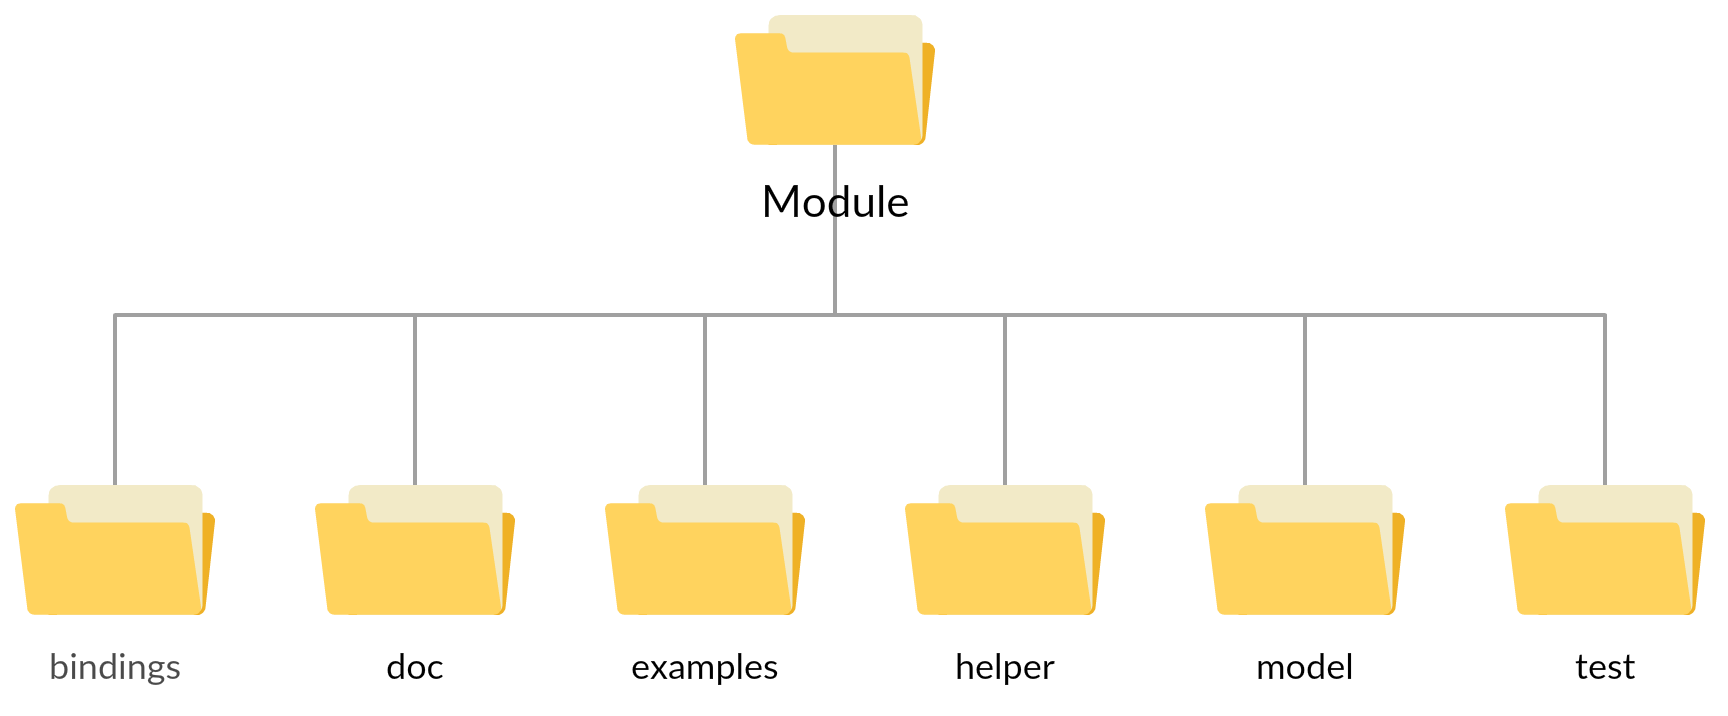
\includegraphics[width=\textwidth]{immagini/ns-3-module}
				\caption{ns-3 module structure}
				\label{fig:ns-3-module}
			\end{figure}
		
			The following directories can be found inside a module's root directory:
			\begin{itemize}
				\item \textbf{bindings:} Python bindings used to make the module's API compatible with Python;
				\item \textbf{doc:} documentation of the module;
				\item \textbf{examples:} examples and proof of concepts of what can be done using the module;
				\item \textbf{helper:} higher level APIs to make the module easier to use;
				\item \textbf{model:} headers and source files which implement the module's logic; 
				\item \textbf{test:} test suite and test cases to test the module.
			\end{itemize}
		
		\subsection{Key elements}
			The element at the base of ns-3 is called \textit{node}, instance of \texttt{ns3::Node}. A node can be thought of as a shell of a computer. Various other elements can be added to nodes, such as:
			\begin{itemize}
				\item NetDevices (e.g. NICs), which enable nodes to communicate over \textit{channels};
				\item protocols;
				\item applications. 
			\end{itemize}
			It is the last those which implement the logic of a simulation. For example, the \texttt{UdoEchoClientApplication} and \texttt{UdpEchoServerApplication} can be used to implement a client/server application which exchange and print the packets' content over the network. The Fast Broadcast protocol has been implemented as an application as well.
			
			
			The \textit{channels} model various type of transmission media, such as the wired and the wireless ones.
			
		\subsection{Structure of a simulation}
			A simulation can be implemented in many ways, but in most cases the following steps are executed:
			\begin{itemize}
				\item manage command line arguments (e.g. number of nodes to consider in the simulation, transmission range, etc.);
				\item initialize all the necessary fields in classes;
				\item create nodes;
				\item set up physical and MAC layers;
				\item set up link layer, routing protocols and addresses;
				\item configure and install applications on nodes;
				\item position nodes and (optionally) give them a mobility model;
				\item schedule user defined events, such as transmissions of packets;
				\item start the simulation;
				\item collect and manage output data.
			\end{itemize}
		
		\subsection{NetAnim}
			Netanim is an offline animator tool based on the Qt toolkit. It collects an XML tracefile during the execution of a simulation and can be used to animate the simulation, analyzing packet transmissions and contents.
			
			\begin{figure}[H]
				\centering
				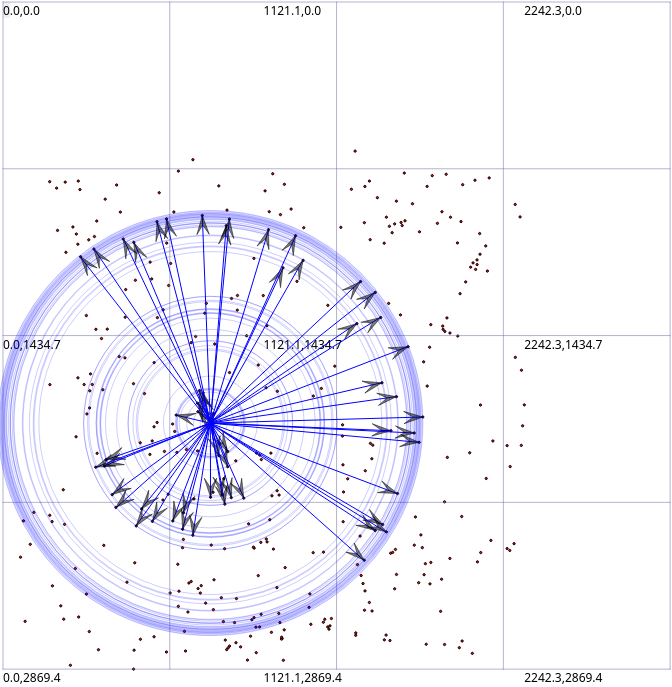
\includegraphics[scale=0.38]{immagini/netanim}
				\caption{Packet transmission in NetAnim}
				\label{fig:netanim}
			\end{figure}
		
	\section{Simulation of Urban MObility}
		Simulation of Urban MObility is an open-source road traffic simulation package. It is written in C++ and licensed under GPLv3. 
		
		
		It offers different tools to analyze and manage real maps from the urban mobility point of view, including pedestrian movement and various types of vehicles.
		

		The original work \cite{ROM2017} utilized SUMO to produce, starting from real maps obtained from OpenStreetMap (OSM), two files:
		\begin{enumerate}
			\item a \texttt{.poly} file using the SUMO tool Polyconvert. This file contains information about all the obstacles, such as buildings, useful for the Obstacle Shadowing module.
			\item a \texttt{.ns2mobility} file using the SUMO tool TraceExporter. This file contains information about the vehicles and their positioning. 
		\end{enumerate}
		The process of generating these two files necessary for ns-3 simulations requires some intermediate steps. The full process is represented in \imgref{fig:sumo-process}. 
		
		The original work considered a only a distance of 25 meters between vehicles; this work considers various distances, ranging from 15 to 45 meters. \imgrefcap{fig:sumo-distances}  shows the same scenario (Padua) with different distances between vehicles.

%		TODO tradurre immagine e aggiungere graficamente foreach distance???
		\begin{figure}[H]
			\centering
			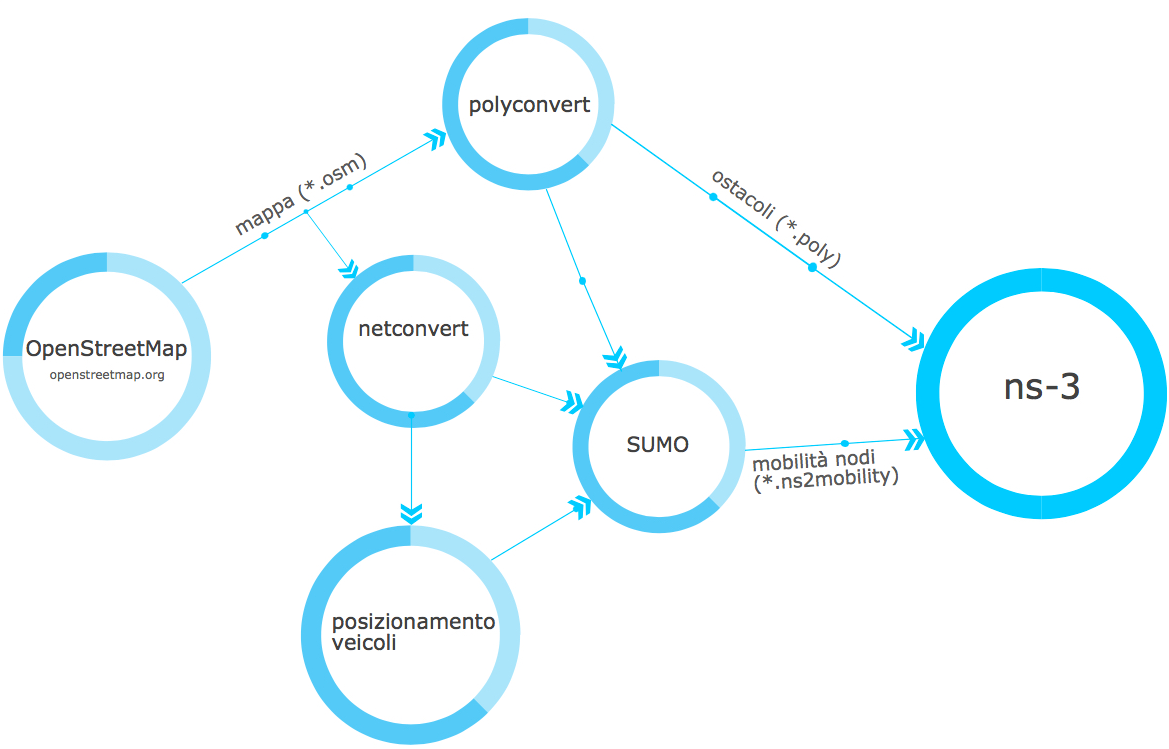
\includegraphics[width=\textwidth]{immagini/sumo-process}
			\caption{Steps to generate necessary files using SUMO (\cite{ROM2017})}
			\label{fig:sumo-process}
		\end{figure}
		
		\begin{figure}[H]
			\centering
			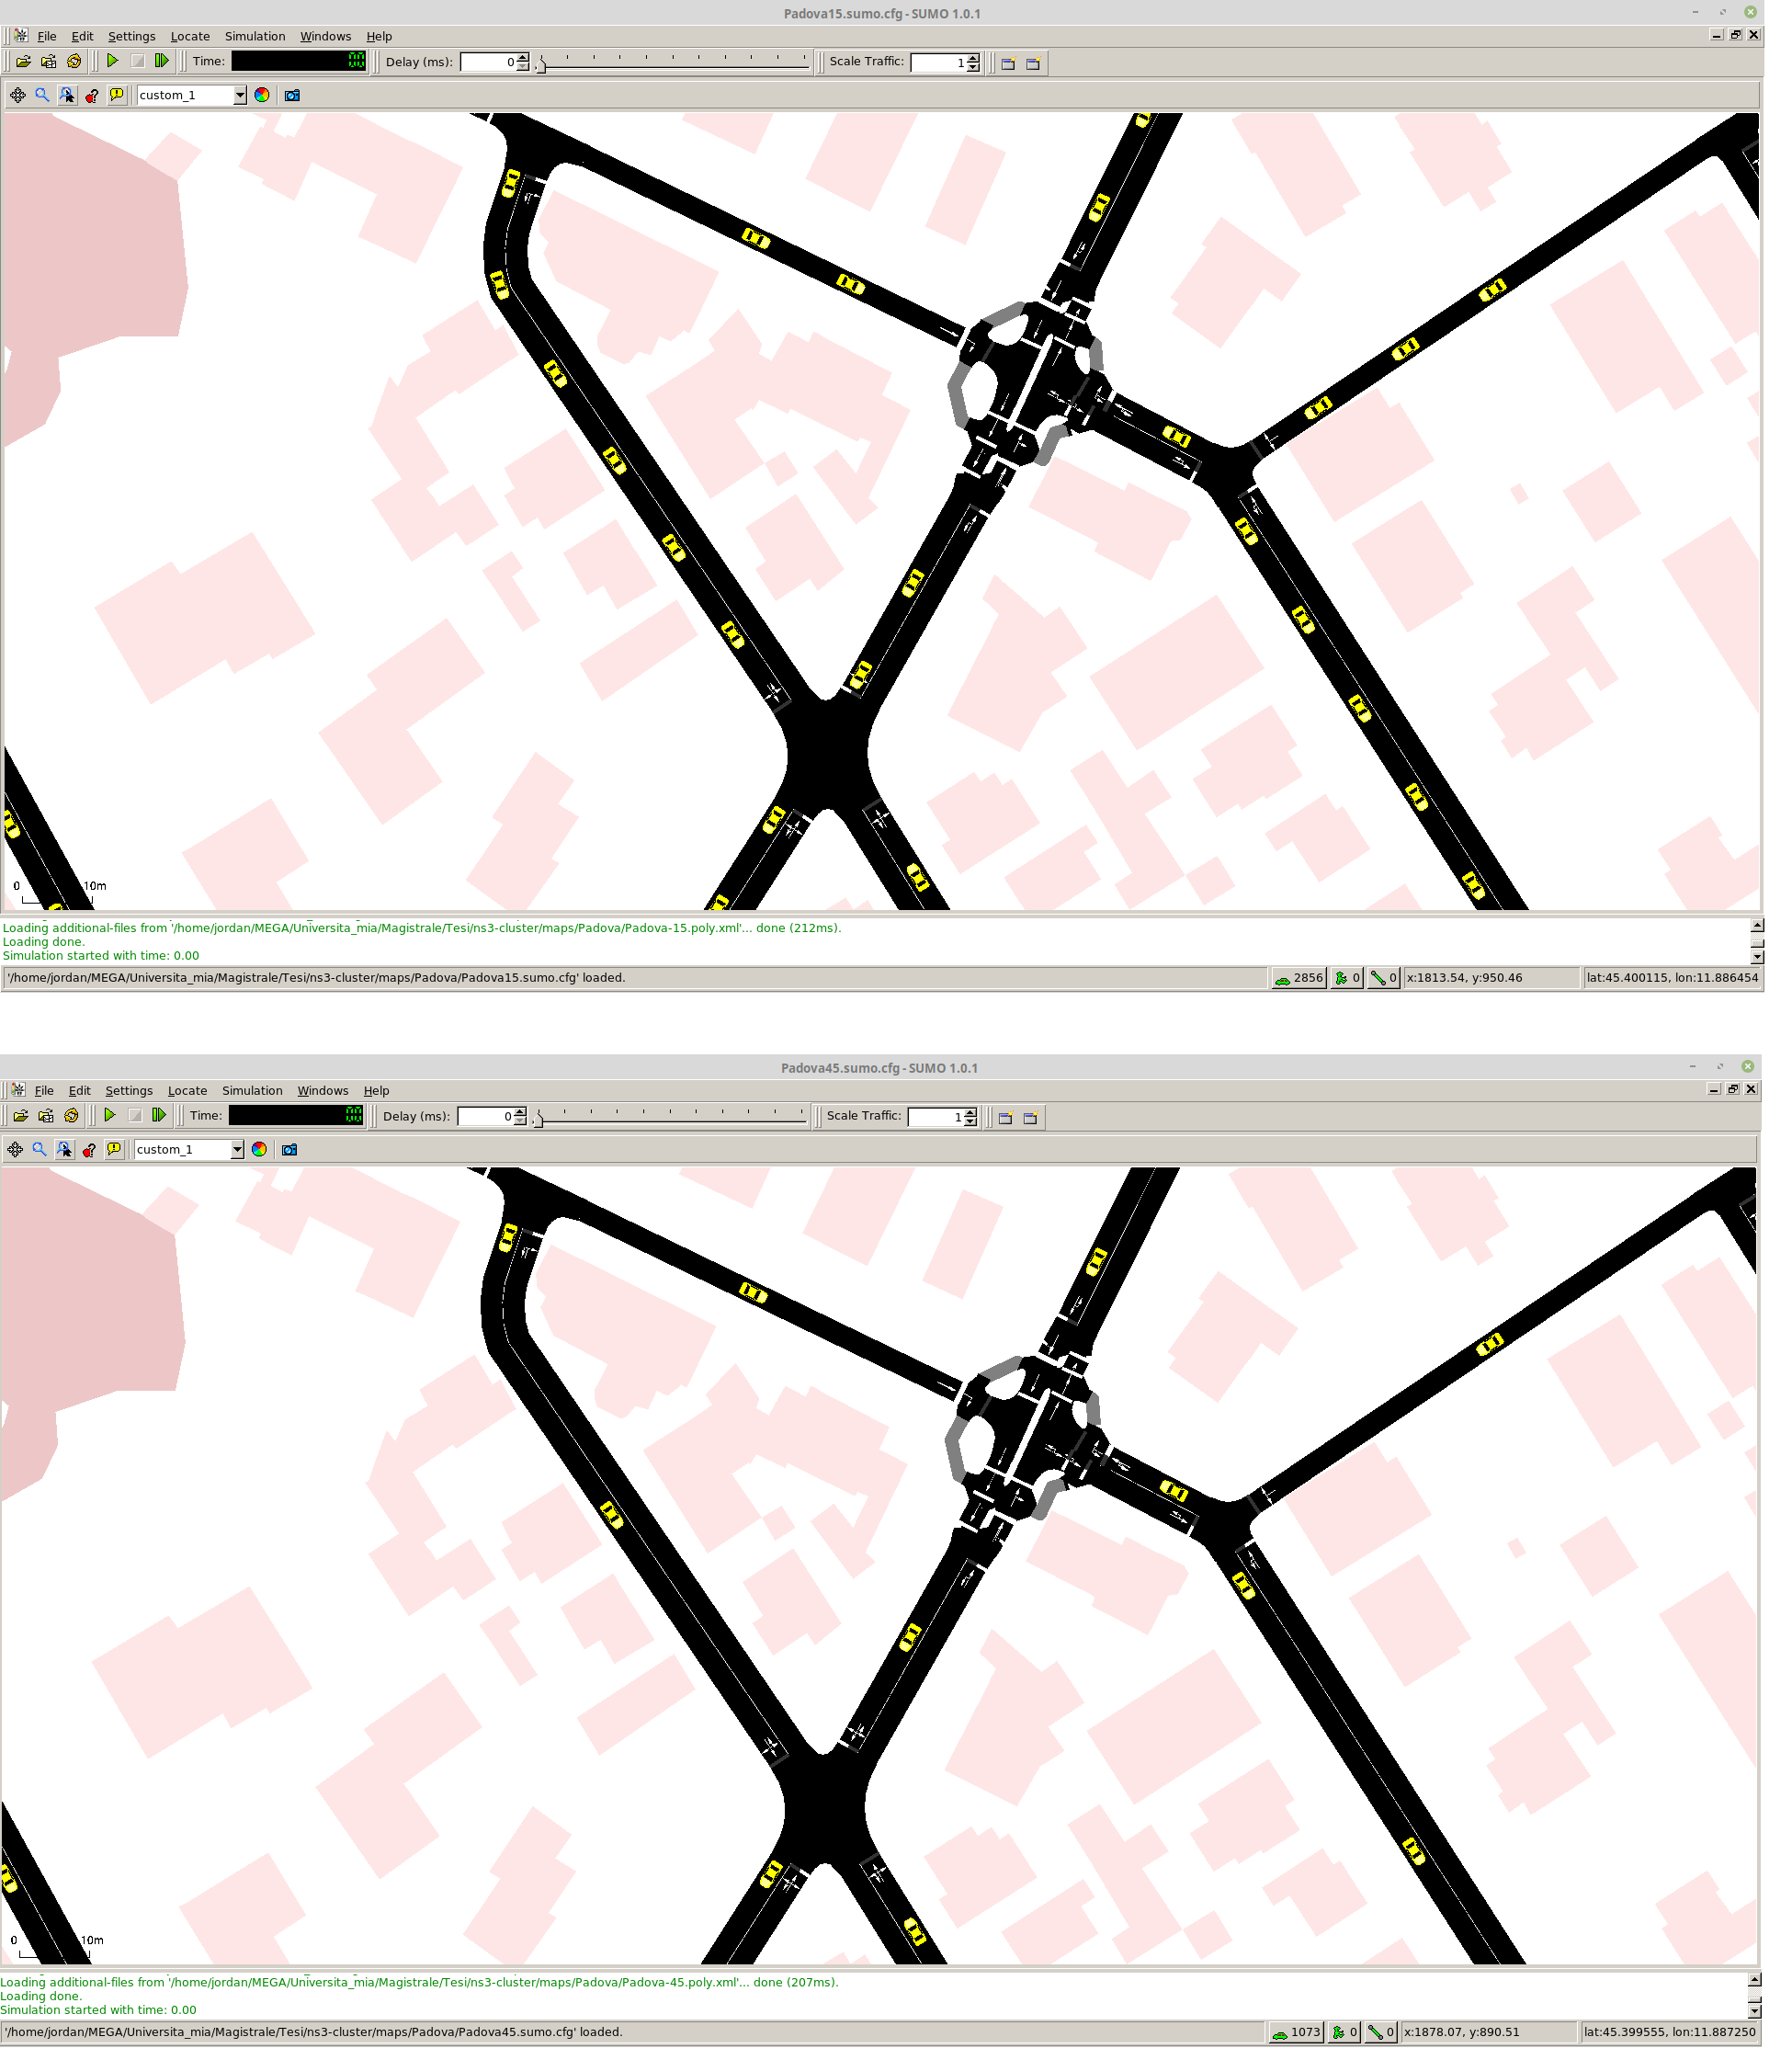
\includegraphics[width=\textwidth]{immagini/sumo-distances}
			\caption{Padua scenario with vehicle distance equals to 15 meters (top) and 45 meters (bottom). Vehicles painted yellow}
			\label{fig:sumo-distances}
		\end{figure}


%
%%**************************************************************
%\chapter{L'azienda}
%\label{cap:lazienda}
%%**************************************************************
%
%%Introduzione al contesto applicativo.\\
%
%%\noindent Esempio di utilizzo di un termine nel glossario \\
%%\gls{api}. \\
%
%%\noindent Esempio di citazione in linea \\
%%\cite{site:agile-manifesto}. \\
%%
%%\noindent Esempio di citazione nel pie' di pagina \\
%%citazione\footcite{womak:lean-thinking} \\
%
%%**************************************************************
%\section{Contesto aziendale}
%
%	IBC è nata nel 1980 come concessionaria \gls{NCR}. Le sue prime attività per conto di NCR riguardavano la fornitura di attrezzature \textit{hardware} per i punti vendita, come ad esempio \gls{POS} e \textit{scanner}. Successivamente, essa si è specializzata nella produzione di \textit{software} specifici per il mercato \gls{retail}, offrendo soluzioni personalizzate in base alle esigenze del singolo cliente.
%	
%	
%	Nel 1995 IBC fonda la sua sede a Peraga di Vigonza, in provincia di Padova. Ha sede tutt'ora nello stesso luogo, con tre filiali ad Alessandria, Trieste e Viterbo.
%	
%	\begin{figure}[H]
%		\centering
%		
\includegraphics[scale=0.7]{immagini/logo-ibc}
%		\caption{Logo IBC (\url{https://www.ibc.it/}).}
%	\end{figure}
%
%	\begin{figure}[H]
%		\centering
%		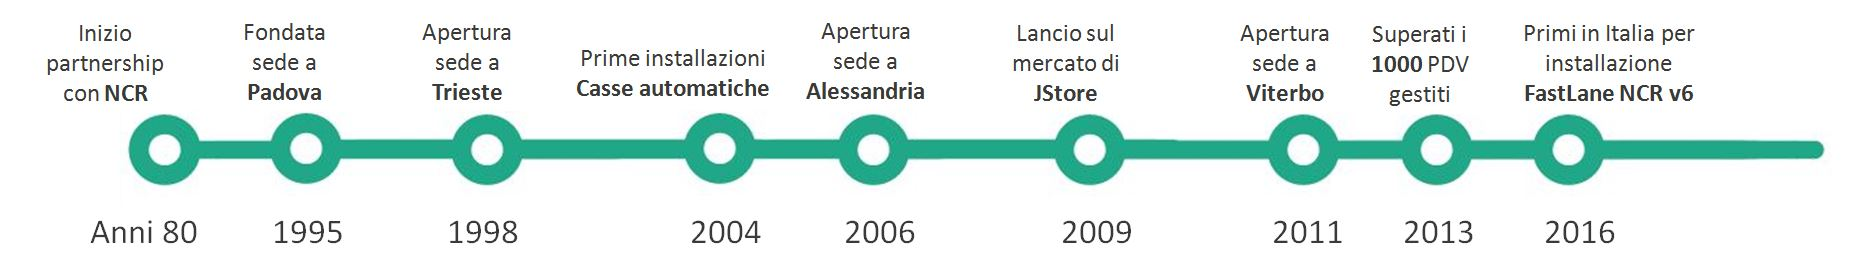
\includegraphics[width=\textwidth]{immagini/cronologia-ibc}
%		\caption{Cronologia IBC (\url{https://www.ibc.it/}).}
%	\end{figure}
%
%	IBC è stata una delle prime \textit{software house} italiane a realizzare progetti riguardanti la \gls{fidelity} e la profilazione dell'utente finale. Correntemente gestisce circa mille punti vendita, avendo installato quattromila casse e quattrocento postazioni \textit{self checkout}. 
%	
%	Attualmente, l'azienda opera principalmente su tre aree:
%	\begin{itemize}
%		\item \textbf{Sviluppo progetti}.
%		\item \textbf{Fornitura prodotti \textit{software} e \textit{hardware}}.
%		\item \textbf{Servizi e assistenza}.	
%	\end{itemize}
%	Fornirò spiegazioni ed esempi riguardo queste aree nelle sezioni successive di questo capitolo.
%	L'azienda possiede inoltre due certificazioni:
%	\begin{itemize}
%		\item \textbf{Certificazione di qualità UNI EN ISO 9001:2008:} per la commercializzazione e l'assistenza di misuratori fiscali, strumenti di pesatura, strumenti per l'automazione del punto vendita e POS bancari.
%		\item \label{laboratorio}
%		 \textbf{Certificazione per la verifica periodica dei misuratori fiscali:} IBC è abilitata alla verificazione periodica dei misuratori fiscali. Inoltre, è anche riconosciuta come laboratorio accreditato presso la CCIAA di Padova per le verifiche metriche degli strumenti di pesatura
%	\end{itemize}
%
%	Per fornire prodotti e servizi aggiornati, l'azienda collabora con vari \textit{partner} tecnologici, tra cui: NCR, Verifone, Motorola, Datalogic, Bizerba, Lenovo e Maind informatica.
%%	\begin{itemize}
%%		\item NCR.
%%		\item Verifone.
%%		\item Motorola.
%%		\item Datalogic.
%%		\item Bizerba.
%%		\item Lenovo.
%%		\item Maind informatica.
%%	\end{itemize}
%	
%	Inoltre, per garantire il servizio di assistenza, l'azienda intrattiene rapporti con: Master Office, InfoMaint, IT-Avantec, BSS, GAB Tamagnini.
%%	\begin{itemize}
%%		\item Master Office.
%%		\item InfoMaint.
%%		\item IT-Avantec.
%%		\item BSS.
%%		\item GAB Tamagnini.
%%	\end{itemize}
%
%	I clienti principali di IBC fanno tutti parte della \gls{GDO}. Tra di essi, troviamo sia clienti nazionali, come ad esempio il Gruppo UniComm, Benetton, Despar, Lando e Rossetto, sia internazionali, come ad esempio Würth Superstore.
%
%	\subsection{Prodotti}
%	I prodotti che IBC fornisce si dividono principalmente in due categorie:
%	\begin{itemize}
%		\item \textit{Hardware}.
%		\item \textit{Software}.
%	\end{itemize}
%
%	\subsubsection*{\textit{Hardware}}
%	I prodotti \textit{hardware} sono costituiti principalmente da strumenti di cassa e di pagamento. L'azienda non produce direttamente questo tipo di prodotti, ma opera da distributore, installatore e manutentore.
%	
%	\begin{enumerate}
%		\item \textbf{Soluzioni \textit{self}:} prodotti che consentono al cliente di concludere la spesa ed effettuare il pagamento autonomamente. Alcuni esempi di questa tipologia di prodotti sono le casse NCR Fastlane Selfserv Checkout Versione 6 (a sinistra nell'immagine) e i Kiosk NCR Selfserv 85 (a destra).
%	
%
%		\begin{figure}[H]
%		\centering
%		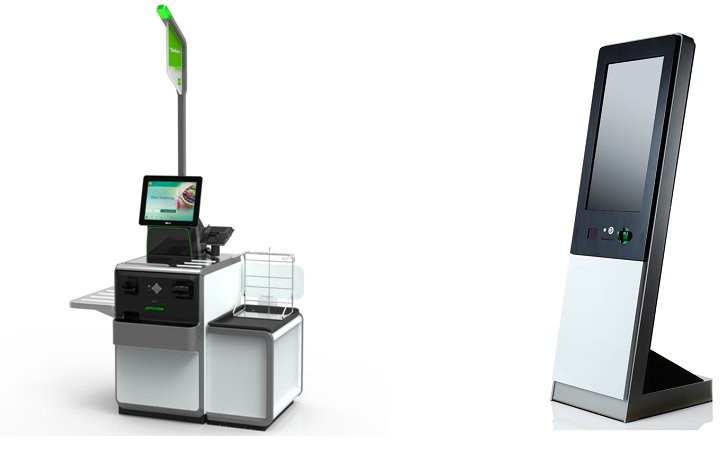
\includegraphics[scale=0.45]{immagini/soluzioni-self}
%		\caption{Soluzioni \textit{self} (\url{https://www.ibc.it/}).}
%		\end{figure}
%	
%		\item \textbf{Soluzioni POS:} si tratta di terminali che permettono al cliente di pagare utilizzando carte di credito, di debito o prepagate.
%	
%		\item \textbf{Periferiche:} \textit{scanner}, stampanti, \textit{monitor} e tutte le altre periferiche per aggiungere funzionalità ai POS e snellire le operazioni di \textit{checkout}.
%		\begin{figure}[H]
%			\centering
%			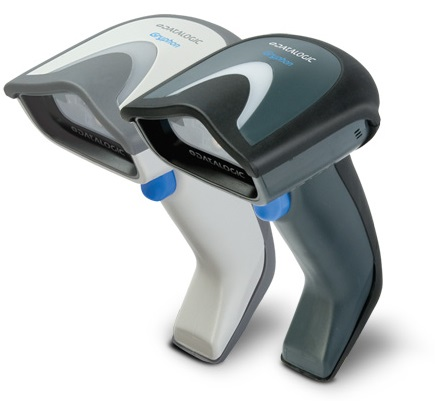
\includegraphics[scale=0.4]{immagini/periferiche}
%			\caption{\textit{Scanner} Datalogic Gryphon M4130 (\url{https://goo.gl/MZqts3}).}
%		\end{figure}
%	
%		\item \textbf{Terminali \textit{mobile}:} palmari che utilizzano sia Android che Windows, in modo da poter fornire compatibilità con la maggior parte dei sistemi dei clienti.
%		
%		\item \textbf{Terminali di pagamento:} strumenti (come ad esempio i PIN Pad) che permettono al cliente di inserire il numero della sua carta durante il pagamento. Garantiscono sicurezza e velocità durante l'esecuzione di questa operazione.
%		\begin{figure}[H]
%			\centering
%			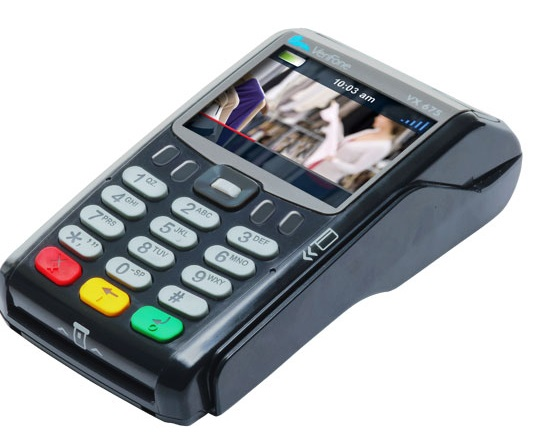
\includegraphics[scale=0.3]{immagini/terminali-di-pagamento}
%			\caption{Pin PAD Verifone VX675 (\url{https://www.ibc.it/}).}
%		\end{figure}
%	
%		\item \textbf{\textit{Server}:} prodotti da installare nei punti vendita. Essi riescono a gestire un elevato numero di richieste concorrenti, caratteristica fondamentale soprattutto nelle operazioni di gestione magazzino.
%		
%		\item \textbf{Bilance:} strumenti che garantiscono alta precisione nella pesatura. Sono inoltre programmabili, personalizzabili e integrabili allo \textit{scanner} per ampliare le funzionalità della postazione cassa. Sono anche utilizzate nella maggior parte dei reparti ortofrutta, permettendo al cliente di effettuare le operazioni di pesatura autonomamente.
%		
%		\begin{figure}[H]
%			\centering
%			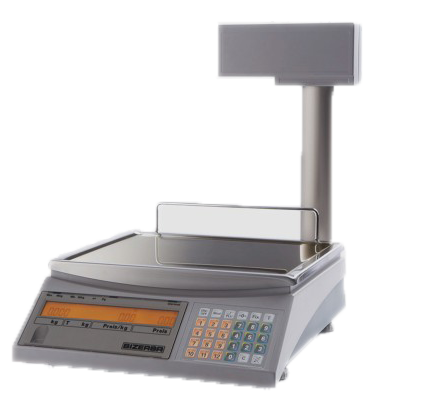
\includegraphics[scale=0.4]{immagini/bilance}
%			\caption{Bilancia Bizerba EC 100 (\url{https://goo.gl/dhTc9F}).}
%		\end{figure}
%	
%	\end{enumerate}
%
%	\subsubsection*{\textit{Software}}
%	
%	Oltre a fornire \textit{hardware}, IBC produce anche \textit{software}. Solitamente i clienti richiedono la realizzazione di soluzioni personalizzate. Per far ciò, l'azienda si è dotata di soluzioni modulari e flessibili.
%	
%	\begin{enumerate}
%		\item \textbf{JStore:} questo \textit{software} è una \textit{suite} completa che offre servizi per gli ambienti \textit{retail}. JStore, una volta installato in sede, permette la gestione e il controllo di tutti i punti vendita. Una delle caratteristiche principali di questo \textit{software} è la sua modularità, in modo da poter essere ampliato e modificato senza intaccare le altre funzionalità. JStore è realizzato in linguaggio Java, quindi è particolarmente adatto ad ambienti multipiattaforma.
%		\begin{figure}[H]
%			\centering
%			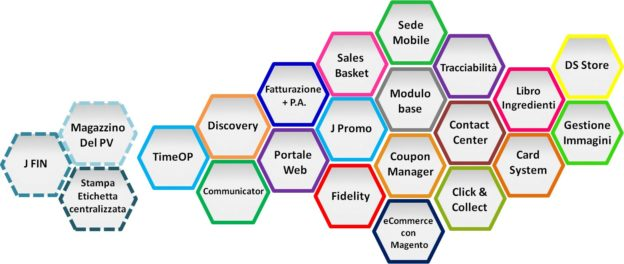
\includegraphics[scale=1.0]{immagini/jstore-moduli}
%			\caption{Moduli JStore (\url{https://www.ibc.it/}).}
%		\end{figure}
%		
%		La \textit{suite} copre quattro aree strategiche principali. Ogni area utilizza vari moduli per fornire le funzionalità necessarie.
%		\begin{enumerate}
%			\item \textbf{\textit{E-commerce}:} la prima area è dedicata agli acquisti via \textit{web}, sia di tipo classico (ovvero dalla creazione dell'ordine \textit{online} fino alla consegna), sia di tipo \gls{clickandcollect}.
%			Quest'area fa utilizzo di due moduli:
%			\begin{figure}[H]
%				\centering
%				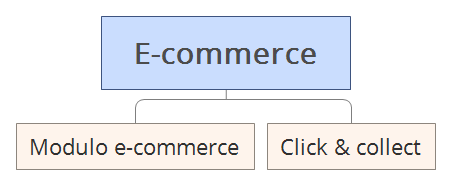
\includegraphics[scale=0.3]{immagini/e-commerce}
%				\caption{Moduli area \textit{e-commerce}}
%			\end{figure}
%		
%			\begin{itemize}
%				\item \textbf{Modulo \textit{e-commerce}:} questo modulo sfrutta un'integrazione della piattaforma di \textit{content management} Magento che gestisce la parte di logistica, preparazione dell'ordine e organizzazione della spedizione integrata con il magazzino.
%				\item \textbf{Modulo \textit{click \& collect}}: si integra con il sistema centrale per la divulgazione anagrafiche e prezzi del cliente, e con gli altri moduli di JStore per la gestione di \textit{fidelity}, \textit{coupon}, promozioni e fatturazione. Il modulo supporta anche \textit{tablet} e \gls{pda}. Inoltre, fornisce funzionalità multispesa (l'operatore può preparare contemporaneamente più spese) e multioperatore (più operatori possono preparare contemporaneamente la stessa spesa).
%			\end{itemize}
%			
%			\item \textbf{\textit{Marketing}:} la seconda area è dedicata alla gestione delle promozioni e dei \textit{coupon}. I moduli di quest'area si occupano di monitorare il flusso di informazioni, generare reportistica e tenere traccia dei \textit{coupon} durante tutti i passaggi di stato.
%			\begin{figure}[H]
%				\centering
%				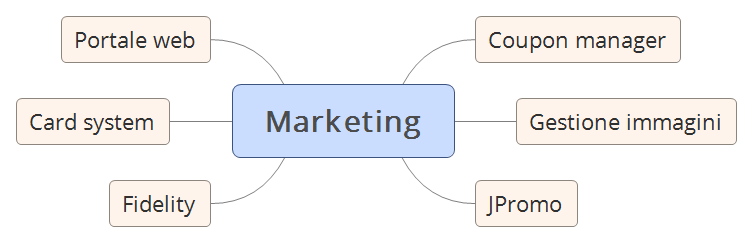
\includegraphics[scale=0.3]{immagini/marketing}
%				\caption{Moduli area marketing}
%			\end{figure}
%		
%			\begin{itemize}
%				\item \textbf{Modulo \textit{coupon manager}:} permette la gestione e la definizione di caratteristiche di valore, fruizione e validità dei buoni spesa.
%				\item \textbf{Modulo gestione immagini:} permette di pubblicare le immagini nei formati richiesti, effettuando il \textit{resize} automatico dell'immagine.
%				\item \textbf{Modulo JPromo:} il modulo si occupa della gestione delle promozioni di negozio. Se utilizzato in ambiente centralizzato, permette di generare un pacchetto promozioni di un'intera catena di negozi.
%				\item \textbf{Modulo \textit{fidelity}:} gestisce in modo centralizzato le funzionalità relative alle carte fedeltà, come ad esempio accumulo e utilizzo punti e ritiri dei premi.
%				\item \textbf{Modulo \textit{card system}:} piattaforma \textit{web} che permette di amministrare le \textit{gift card}.
%				\item \textbf{Modulo portale \textit{web}:} modulo che fornisce un canale di comunicazione tra il punto vendita e il cliente fidelizzato, offrendo varie informazioni su promozioni e saldo punti.
%			\end{itemize}
%		
%		\item \textbf{Gestione operativa del punto vendita:} la terza area soddisfa le esigenze di negozio, dalla fatturazione, la tracciabilità e l'inventario fino alla gestione delle comunicazioni con i clienti.
%		
%		\begin{figure}[H]
%			\centering
%			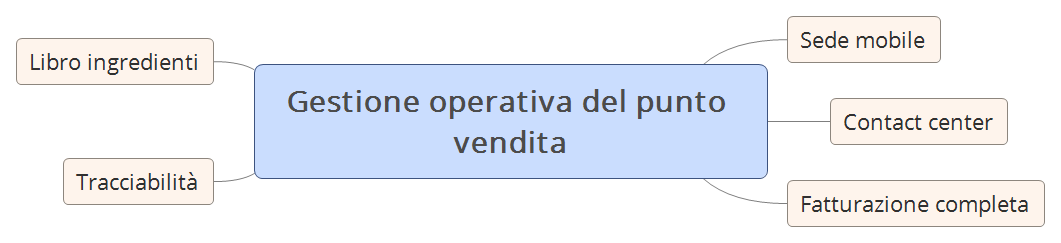
\includegraphics[scale=0.3]{immagini/gestione-operativa}
%			\caption{Moduli gestione operativa del punto vendita}
%		\end{figure}
%		
%		\begin{itemize}
%			\item \textbf{Modulo sede \textit{mobile}:} modulo che gestisce in modo centralizzato l'inventario permanente dei dispositivi mobili.
%			\item \textbf{Modulo \textit{contact center}:} piattaforma \textit{web} in grado di gestire la registrazione delle richieste (come ad esempio i reclami dei clienti), le soluzioni proposte e le risposte dei clienti.
%			\item \textbf{Modulo fatturazione completa:} permette la rilevazione di fatture e scontrini emessi nei punti vendita. Inoltre, supporta l'invio automatico ad intervalli regolari e personalizzabili degli scontrini dal punto vendita alla sede.
%			\item \textbf{Modulo tracciabilità:} modulo che gestisce la tracciabilità dei lotti carne e ittici nei punti vendita.
%			\item \textbf{Modulo libro ingredienti:} il modulo permette di memorizzare e riconoscere gli allergeni presenti all'interno dei prodotti. Questa funzionalità consente la pubblicazione del libro degli ingredienti secondo le normative europee.
%		\end{itemize}
%	
%		\item \textbf{Gestione strategica e di monitoraggio:} la quarta e ultima area comprende tutti i moduli che riguardano l'osservazione e il controllo dei sistemi e delle informazioni. Lo scopo di quest'area è definire le strategie di gestione, come la produttività del lavoro dei cassieri e i dati del venduto.
%		
%		\begin{figure}[H]
%			\centering
%			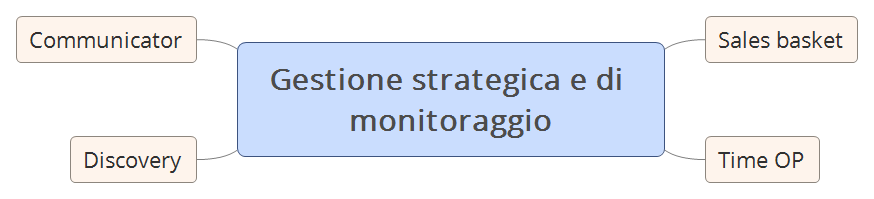
\includegraphics[scale=0.3]{immagini/gestione-strategica}
%			\caption{Moduli gestione strategica e di monitoraggio}
%		\end{figure}
%		
%		\begin{itemize}
%			\item \textbf{Modulo \textit{sales basket}:} strumento che permette di analizzare le informazioni sul venduto a partire dagli scontrini. Supporta l'attivazione di \textit{alert} in base a eventi, con la possibilità di inviare messaggi via SMS o \textit{e-mail}.
%			\item \textbf{Modulo \textit{time OP}:} modulo che permette l'analisi delle casse, fornendo dati sulla produttività del lavoro dei cassieri e consentendo di effettuare comparazioni tra i punti vendita della catena.
%			\item \textbf{Modulo \textit{discovery}:} si occupa di monitorare e recuperare le informazioni tecniche e di stato dei sistemi, inviando segnalazioni di errori quando necessario.
%			\item \textbf{Modulo \textit{communicator}:} modulo per la gestione e il monitoraggio della divulgazione di informazioni in JStore.
%		\end{itemize}
%	
%		\end{enumerate}
%
%
%		\item \textbf{i\_STORE:} \textit{software} di \gls{backoffice} che permette di gestire dalla sede le principali esigenze dei punti vendita. È particolarmente adatto alle aziende del settore distributivo, dato il \textit{focus} sulla movimentazione delle merci. Uno dei vantaggi principali di i\_STORE è il funzionamento in modo indipendente rispetto ai modelli di casse e bilance installate nel punto vendita.
%			
%		\begin{figure}[H]
%			\centering
%			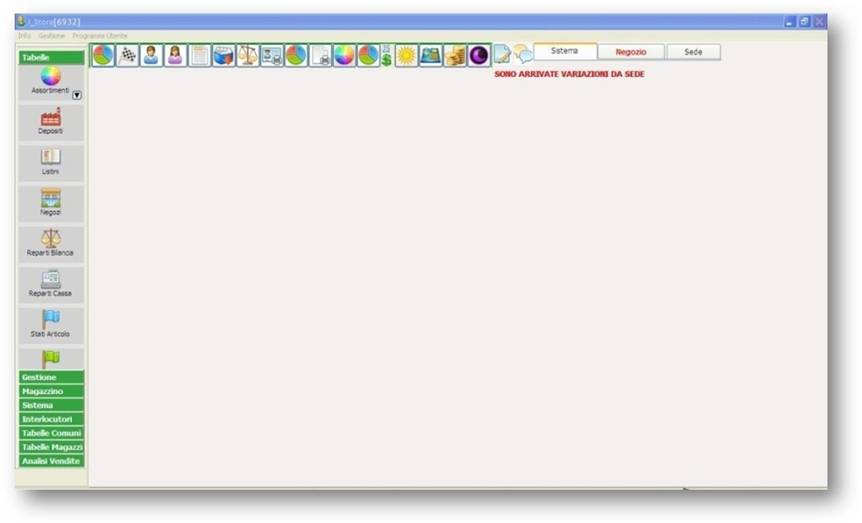
\includegraphics[scale=0.4]{immagini/i-store}
%			\caption{\textit{Screenshot} di i\_STORE (\url{https://www.ibc.it/}).}
%		\end{figure}
%	
%		\item \textbf{ARS:} \textit{software} realizzato da NCR e installato da IBC. Questo \textit{software} è installato su casse tradizionali e \textit{self-checkout}, indipendentemente dall'\textit{hardware} e dal sistema operativo. Gestisce l'applicazione delle logiche promozionali durante la vendita e il pagamento.
%		
%		\item \textbf{UPB:} \textit{software} NCR che permette alle casse di offrire vari servizi, come il pagamento di utenze, tasse di abilitazione di carte prepagate e la possibilità di effettuare ricariche telefoniche. Con questo \textit{software} è possibile portare a termine, durante il pagamento in cassa, qualsiasi attività che tipicamente viene svolta dalla tabaccheria o dalle poste.
%		
%		\item \textbf{WinEPTS}: è un \textit{software} NCR per i pagamenti elettronici che consente al \textit{retailer} di rendersi completamente autonomo dalle banche, diminuendo (e in alcuni casi azzerando) le commissioni sui pagamenti effettuati tramite bancomat.
%		
%		\item \textbf{Customer Point:} soluzione IBC installata su Kiosk per permettere al cliente di avere informazioni su prodotti e servizi. Il \textit{software} è anche integrabile su dispositivi \textit{touch}.
%		
%		\begin{figure}[H]
%			\centering
%			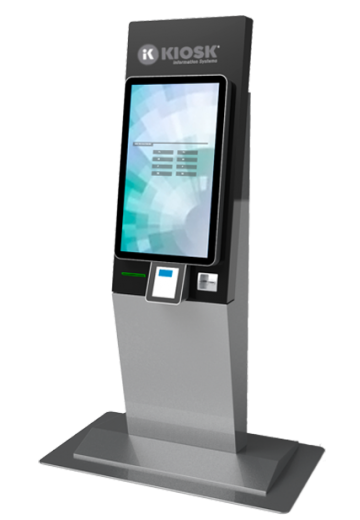
\includegraphics[scale=0.4]{immagini/kiosk}
%			\caption{Un Kiosk (\url{https://goo.gl/PhTxdc}).}
%		\end{figure}
%		
%		\item \textbf{MobileStore:} \textit{app mobile} per la raccolta remota dei dati del punto vendita. Supporta la lettura dei codici a barre e la memorizzazione di informazioni, effettuandone anche una prima elaborazione direttamente sul terminale.
%		
%		\item \textbf{Libro guida ordini:} \textit{app mobile} disponibile su \textit{tablet} che permette il riordino degli articoli in maniera digitale, sostituendo il tradizionale libro cartaceo ed eliminandone i costi di gestione.
%		
%		\item \textbf{Assistente di negozio:} \textit{app mobile} mirata a dare supporto al cliente nella vendita \textit{no food}. Il \textit{software} permette di dare informazioni e caratteristiche tecniche dei prodotti accedendo direttamente all'anagrafica di sede.
%		
%		\item \textbf{Fidelity:} \textit{app mobile} per la gestione delle carte fedeltà rivolta al cliente. L'installazione dell'applicazione è semplificata in quanto è possibile installarla rilevando direttamente il QR \textit{code}. Attraverso l'\textit{app} il cliente può compiere varie operazioni, come ad esempio prenotare la spesa, gestire i \textit{coupon} e visualizzare gli scontrini.
%		
%		\item \textbf{Yourself:} \textit{app} installabile sui lettori portatili in grado di scannerizzare i codici a barre dei prodotti, in modo da velocizzare il pagamento in cassa. Collegandosi a JStore, l'applicazione permette al cliente di evitare la fila alle casse, offrendogli la possibilità di imbustare direttamente la spesa.
%	\end{enumerate}
%	
%	\subsection{Servizi}
%		Nel mercato odierno, i prodotti non sono l'unica caratteristica che permette ad un'azienda di aver successo. Data la collaborazione, in molti casi pluriennale, tra IBC e i suoi clienti, l'azienda fornisce vari servizi. 
%		
%		\begin{enumerate}
%			\item \textbf{Assistenza:} IBC fornisce assistenza \textit{software} e \textit{hardware} attraverso servizi di \textit{call center}, \textit{help desk} e interventi \textit{on-site}. Una delle caratteristiche di forza dell'assistenza IBC è la gestione delle segnalazioni in tempi brevi e garantiti. Per garantire ciò, l'azienda rimane aperta quasi tutto l'anno, compresi i \textit{weekend}. 
%			
%			\begin{figure}[H]
%				\centering
%				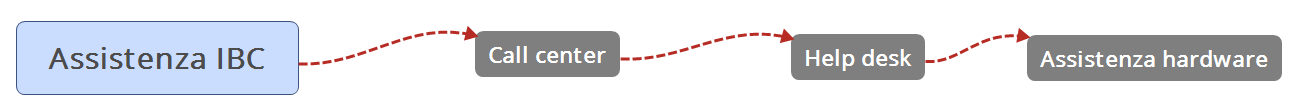
\includegraphics[width=\textwidth]{immagini/assistenza}
%				\caption{Percorso assistenza IBC.}
%			\end{figure}
%		
%			Una richiesta di assistenza a IBC attraversa vari stadi:
%			\begin{enumerate}
%				\item \textbf{\textit{Call center}:} riceve e registra le richieste di assistenza, indicandone l'urgenza e assegnando un codice identificativo. Successivamente, inoltra la chiamata ai tecnici di \textit{help desk}.
%				\item \textbf{\textit{Help desk}:} analizza il problema tecnico dichiarato e fornisce una soluzione per via telefonica. Nel caso la soluzione non sia efficace o l'\textit{help desk} non abbia strumenti o competenze sufficienti, quest'ultimo assegna la risoluzione della segnalazione al reparto IBC più adatto.
%				\item \textbf{Assistenza \textit{hardware}:} qualora il problema segnalato sia di natura \textit{hardware}, il personale incaricato provvede ad effettuare le operazioni di manutenzione necessarie e ripristina le normali condizioni di funzionamento presso la sede del cliente.
%			\end{enumerate}
%			
%			\item \textbf{Laboratorio metrologico:} come descritto in \ref{laboratorio}, IBC è anche laboratorio accreditato presso la CCIAA di Padova per le verifiche metriche degli strumenti di pesatura. I servizi offerti riguardano la verifica periodica prevista per legge di bilance e strumenti per la pesatura, sia automatici che non. La verifica, oltre che alla scadenza, è obbligatoria anche dopo un'attività di manutenzione che ha rimosso i sigilli dallo strumento.
%			
%			
%			In aggiunta ai servizi previsti per legge da un laboratorio metrologico, IBC offre in aggiunta servizi ulteriori, come ad esempio il trasporto delle masse necessarie per effettuare le prove, la conservazione dei dati presso l'archivio aziendale e la gestione automatica della periodicità delle scadenze. Inoltre, per legare il servizio di assistenza al servizio di laboratorio, nel caso di bilance che non risultino idonee alla verifica periodica, IBC offre gratuitamente la seconda uscita dell'ispettore metrico per l'intervento di riparazione. 
%		\end{enumerate}
%		
%\section{Organizzazione aziendale}
%	\subsection{Organizzazione e reparti}
%		IBC, internamente, è divisa in due macro aree:
%		\begin{itemize}
%			\item \textbf{Amministrativa:} area che comprende le funzioni aziendali di amministrazione, risorse umane, organizzazione e finanza.
%			\item \textbf{Prodotti e assistenza}: area che comprende lo sviluppo di prodotti, principalmente \textit{software}, e l'assistenza post vendita.
%		\end{itemize}
%		
%		Essendo stato collocato all'interno del team Java 3 per lo svolgimento dello \textit{stage}, ho potuto comprendere meglio il funzionamento dell'area prodotti e assistenza. Per questo motivo mi concentrerò maggiormente sull'analisi di quest'area. In aggiunta a ciò, ho avuto rapporti molto limitati con l'area amministrativa, per cui non sono in grado di fare un'analisi approfondita del funzionamento interno di quest'ultima.
%		
%		L'area prodotti e assistenza è suddivisa in vari reparti:
%		\begin{itemize}
%			\item \textbf{Reparto Analisi:} reparto che si occupa di comprendere le necessità dei clienti e formulare un'analisi comprensibile dal personale tecnico aziendale. Gli analisti sono il primo passo verso la formulazione di una soluzione \textit{software}. Questo reparto opera sia presso il cliente che presso la sede IBC.
%			\item \textbf{Reparto Sviluppo:} reparto che si occupa della realizzazione effettiva del prodotto finale, utilizzando varie tecnologie e linguaggi di programmazione. Il reparto sviluppo è composto da:
%			\begin{itemize}
%				\item Tre \textit{team} Java, che si occupano della realizzazione di \textit{web app} e dello sviluppo di JStore.
%				\item Un \textit{team} \textit{device}, le cui mansioni sono la realizzazione e la manutenzione delle applicazioni \textit{mobile}.
%				\item Un \textit{team} che si occupa della realizzazione e manutenzione del \textit{software} delle casse.
%			\end{itemize}
%			\item \textbf{Reparto \textit{Customer Care} e \textit{Help Desk}}: reparto che si occupa dell'assistenza post vendita, sia su prodotti \textit{hardware} che \textit{software}. Ho potuto notare che molte segnalazioni di natura \textit{software} vengono fatte risolvere al reparto sviluppo, spesso provocando ritardi in altre attività.
%		\end{itemize}
%		Nell'elenco mancano reparti come Ricerca e Sviluppo e reparti che si occupano di progettazione. Questa mancanza è dovuta al fatto che IBC non ha dei reparti dedicati per questi scopi, ma si affida a singoli dipendenti (o in ogni caso gruppi molto ristretti) che non costituiscono reparti a sé stanti. Ho potuto notare questa propensione anche in relazione al mio \textit{stage}: per l'azienda, le attività da me svolte rientrano nella funzione ricerca e sviluppo. Fornirò maggiori informazioni su questo punto, insieme ad altri obiettivi aziendali legati agli \textit{stage}, nel capitolo \ref{cap:loffertadistage}.
%		
%		
%		La tendenza nel far prendere decisioni importanti ad un numero ristretto di persone si sposa con la struttura aziendale che ho potuto rilevare. Anche se giuridicamente IBC si presenta come una S.r.l.,  nella pratica il suo funzionamento è quello di un'impresa a conduzione familiare, data la consanguineità dei ruoli di più alto livello.
%		 
%		Tra i vantaggi di questo approccio ho potuto notare la facilità nel prendere decisioni anche importanti in tempi relativamente brevi. Se le stesse decisioni avessero dovuto attraversare vari organi aziendali prima di essere prese, sicuramente sarebbe passato molto più tempo e alcune avrebbero riportato una perdita di efficacia.
%		Gli svantaggi principali sono invece: 
%		\begin{itemize}
%			\item Troppe libertà e responsabilità lasciate al personale tecnico, specialmente ai programmatori. Data la mancanza di un reparto che si occupa di progettazione di dettaglio, il programmatore ha troppa libertà decisionale su come implementare la soluzione che gli viene assegnata. Alcune volte ho potuto notare come decisioni prese da un programmatore abbiano causato incomprensioni e ritardi nelle attività di altri \textit{team} di sviluppo.
%			\item Ritardi e impossibilità nel prendere decisioni di natura architetturale quando anche soltanto uno dei (pochi) dipendenti che si occupa di progettazione è assente.
%		\end{itemize}
%	
%	\subsection{Processi}
%		Il modello di sviluppo che IBC ha adottato si rifà ai principi del modello Agile, consultabili al seguente indirizzo:
%		\begin{center}
%			\url{http://agilemanifesto.org/iso/it/principles.html}
%		\end{center}
%		
%		\begin{figure}[H]
%			\centering
%			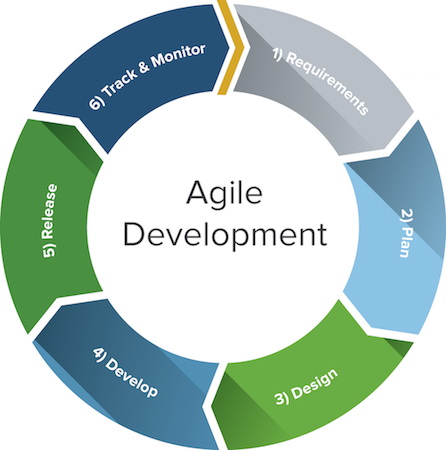
\includegraphics[scale=0.4]{immagini/ciclo-agile}
%			\caption{Ciclo di sviluppo Agile (\url{https://goo.gl/ESua3X}).}
%		\end{figure}
%		
%		I principi che ho percepito come i più seguiti sono:
%		\begin{itemize}
%			\item \jquote{Committenti e sviluppatori devono lavorare insieme
%			quotidianamente per tutta la durata del progetto}. Ho constatato che il personale tecnico di alcuni clienti di IBC ha contatti quotidiani con i programmatori dell'azienda, fino ad arrivare ad influenzare il modo con cui le funzionalità sono implementate.
%			\item \jquote{Una conversazione faccia a faccia è il modo più efficiente e più efficace per comunicare con il \textit{team} ed all'interno del \textit{team}}. Nonostante l'utilizzo di \textit{software} di \textit{ticketing} e la presenza di procedure ben definite per il contatto tra membri di \textit{team} diversi, il personale predilige un rapporto faccia a faccia la maggior parte delle volte. In molti casi ho potuto rilevare che problemi di incomprensioni tra sviluppatori sono stati risolti in modo molto efficace semplicemente parlando di persona.
%		\end{itemize}
%		
%		Tuttavia, IBC non segue i principi alla lettera, ma adatta le sue reazioni a seconda del caso. Ad esempio, l'azienda non accetta cambiamenti sostanziali nei requisiti anche a stadi avanzati dello sviluppo. Nel caso in cui ciò avvenisse, il cliente dovrebbe pagare una somma di denaro per finanziare le ore aggiuntive necessarie a sviluppare (o modificare) il \textit{software} in modo che copra le nuove richieste. Personalmente sono d'accordo con questa linea di pensiero.
%		
%		
%		Un altro punto di distacco tra il modello adottato da IBC e Agile sono le riunioni. Contrariamente alla prassi adottata dal modello Agile, ovvero riunioni giornaliere (\textit{Daily standup meeting}), IBC tiene riunioni settimanali. 
%		
%		
%		Tenendo conto di questi (e altri) punti, ho potuto percepire che l'azienda non adotta ciecamente il modello Agile, ma ne sfrutta solamente i punti di forza, tralasciando completamente le \jquote{cerimonie} che la metodologia è solita portare con sé. 
%		
%		
%		
%	\subsection{Progetti}
%		Il lavoro all'interno dell'azienda è organizzato a progetti. Ogni \textit{team} si trova a lavorare contemporaneamente a più progetti, richiedendo un cambio di contesto a volte molto rapido. 
%		
%		
%		 Per quanto riguarda il \textit{team} Java con cui ho lavorato a più stretto contatto, ho potuto notare che, oltre ai progetti, il \textit{team} doveva gestire anche l'infrastruttura e alcuni moduli di JStore. Nonostante la differenziazione dei \textit{task} assegnati e i molti ambiti gestiti, i membri del gruppo hanno quasi sempre gestito il lavoro in modo organizzato. Questo denota una buona organizzazione all'interno del \textit{team}.
%		 Talvolta, più \textit{team} hanno dovuto lavorare su moduli differenti dello stesso progetto e anche in quei casi la comunicazione si è dimostrata efficace.
%		 
%		
%\section{Tecnologie a supporto dei processi}
%	\begin{figure}[H]
%		\centering
%		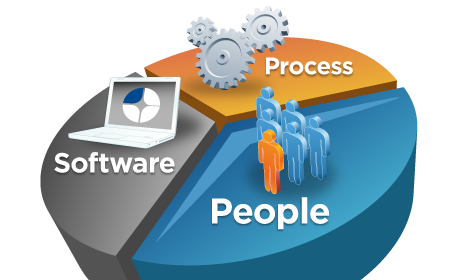
\includegraphics[scale=0.4]{immagini/tecnologie-processi}
%		\caption{Persone, processi e tecnologie (\url{https://goo.gl/KX59QR}).}
%	\end{figure}
%	Con l'aumentare delle dimensioni di un'azienda, quest'ultima ha sempre più bisogno di tecnologie che supportino i processi. Infatti, nonostante le persone siano una parte fondamentale per il raggiungimento degli obiettivi aziendali, le tecnologie aiutano sia a rendere il raggiungimento di tali obiettivi ripetibile sia a contenere i costi.
%	
%	\subsection{Gestione di progetto}
%		\subsubsection*{SysAid}
%			\begin{figure}[H]
%				\centering
%				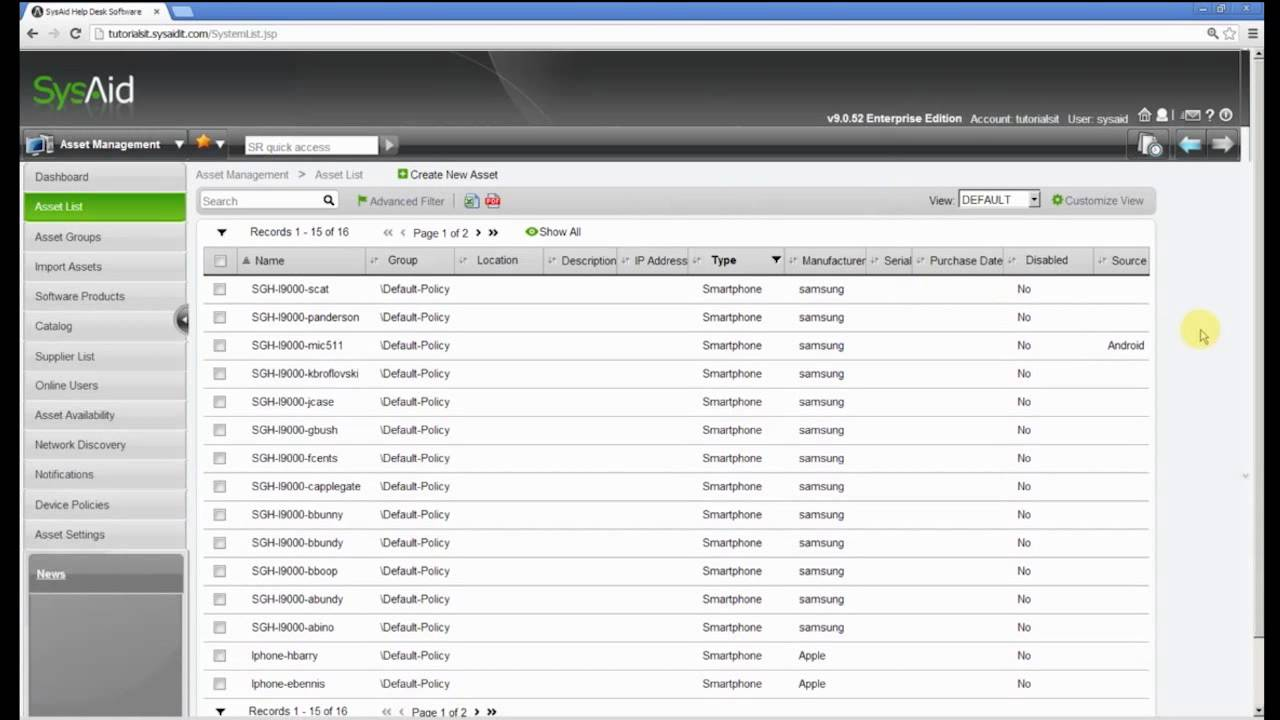
\includegraphics[width=\textwidth]{immagini/sysaid}
%				\caption{\textit{Screenshot} di SysAid (\url{https://goo.gl/cACkfo}).}
%			\end{figure}
%			Il principale strumento adottato da IBC per la gestione di progetto è SysAid. SysAid è un \textit{software} di \textit{help desk} completo, utilizzato in quasi ogni reparto IBC. Questo \textit{software} offre varie funzionalità ed è integrabile anche su dispositivi \textit{mobile}. Ecco un elenco delle sue principali caratteristiche:
%			\begin{itemize}
%				\item \textbf{Gestione \textit{ticket}:} SysAid permette di inserire \textit{ticket} e di chiuderli una volta risolti. Questa funzionalità permette al reparto sviluppo di IBC di ricevere \textit{ticket} direttamente dal reparto \textit{customer care} e \textit{help desk} e di risolverli in autonomia, qualora non ci siano incomprensioni o problemi più gravi.
%				Il \textit{software} fornisce anche funzionalità di notifica e di regolazione delle priorità.
%				\item \textbf{Gestione \textit{asset}:} funzionalità che permette di rilevare automaticamente e gestire i dispositivi collegati alla rete aziendale.
%				\item \textbf{\textit{Knowledge base}:} permette di memorizzare documentazione e guide che consentono la risoluzione dei problemi più frequenti.
%				\item \textbf{Gestione \textit{dashboard}:} SysAid offre un rapporto in tempo reale dello stato dei \textit{ticket} e permette di avere \textit{report} di vario genere.
%			\end{itemize}
%
%	\subsection{Gestione della configurazione e versionamento}
%		\label{sec:configurazione}
%		\subsubsection*{SVN}
%			\begin{figure}[H]
%				\centering
%				
\includegraphics[scale=2.0]{immagini/svn}
%				\caption{Gestione centralizzata di SVN (\url{https://goo.gl/67AyyR}).}
%			\end{figure}
%		
%				Il sistema di versionamento utilizzato da IBC è Subversion (d'ora in poi SVN). Questo sistema offre un \textit{repository} centralizzato su cui gli sviluppatori effettuano dei \textit{commit} per pubblicare i cambiamenti da loro prodotti.
%				Alcune caratteristiche di SVN sono:
%				\begin{itemize}
%					\item L'atomicità dei \textit{commit}: qualora un \textit{commit} dovesse essere interrotto, il \textit{repository} non verrebbe lasciato in uno stato di inconsistenza.
%					\item Un'efficiente gestione dei \textit{file} binari.
%					\item Il \textit{branching} è un'operazione che richiede un tempo indipendente dalla dimensione dei dati.
%					\item La licenza è \gls{opensource}.
%				\end{itemize}
%				La centralizzazione di SVN, la caratteristica principale che garantisce la sua semplicità rispetto a soluzioni distribuite come Git, è anche il suo principale svantaggio. Infatti, in caso di impossibilità di accesso al \textit{repository}, è impossibile effettuare \textit{commit} e la gran parte delle funzionalità di versionamento è inutilizzabile. IBC sopperisce a questo rischio fornendo una connessione \textit{internet} affidabile all'interno dei propri stabili.
%				
%		\subsubsection*{Maven}
%			Apache Maven è un \textit{software} utilizzato per la gestione della configurazione e delle dipendenze tra un progetto e librerie esterne. In IBC viene utilizzato per gestire i progetti Java, anche se è possibile configurarlo per altri linguaggi.
%			Alla base di Maven c'è il POM (Project Object Model), ovvero un \textit{file} XML che descrive le \textit{directory} di progetto, le dipendenze e definisce come deve avvenire il processo di \textit{build}. Il \textit{download} delle dipendenze è gestito in modo automatico, tipicamente appoggiandosi ad un \textit{repository} centralizzato.
%			
%	\subsection{Sviluppo}
%		\label{sec:sviluppo}
%		\subsubsection*{Wicket}
%			Apache Wicket è un \textit{framework} \textit{web} lato \textit{server} che utilizza Java per lo sviluppo di \textit{web app}. Il \textit{framework} fornisce un insieme di componenti grafiche pronte all'uso, che permettono un'alta produttività a discapito della personalizzazione. 
%			Wicket risulta essere adatto allo sviluppo di \textit{web app} per conto dei clienti di IBC. Infatti, la maggior parte delle funzionalità richieste dai clienti è già implementata e gestita dai componenti di Wicket, minimizzando lo sviluppo di componenti personalizzate. 
%		
%	\begin{table}[H]
%		\centering
%		\begin{tabularx}{\textwidth}{|X | X | X | X | X |}
%			\hline
%			\rowcolor{lightgray}
%			\textbf{Gestione di progetto} & \textbf{{Config.} e \mbox{versionamento}} &  \textbf{Sviluppo} &  \textbf{IDE} &  \textbf{Vari}  \\
%			\hline
%			SysAid & SVN & Java & Eclipse & LibreOffice \\
%			\hline
%			& Maven & C++ & Android Studio & Skype \\
%			\hline
%			& Ant & Wicket & & \\
%			\hline
%			& & Bootstrap & & \\
%			\hline
%			& & Hibernate & & \\
%			\hline
%		\end{tabularx}
%	\caption{Principali tecnologie utilizzate da IBC.}
%	\end{table}
%	
%\section{Rapporto con l'innovazione}
%	Negli ultimi anni, il mondo del \textit{retail} in Italia sta avanzando in termini tecnologici. Le casse automatiche sono sempre più diffuse all'interno dei punti vendita e, con l'espansione di supermercati e ipermercati, molti clienti sentono la necessità di avere servizi aggiuntivi, come le ricariche telefoniche o i servizi tipici delle tabaccherie. 
%	
%	
%	IBC, per poter fornire soluzioni adatte alle richieste del mercato e dei clienti, necessita di stare al passo dal punto di vista tecnologico. Questo è il motivo per cui intrattiene rapporti con alcuni dei fornitori che offrono tecnologie più avanzate, come ad esempio NCR e Motorola. Queste collaborazioni permettono la fornitura e la manutenzione di \textit{hardware} sempre aggiornato.
%	
%	
%	Anche lo sviluppo di soluzioni multipiattaforma è uno dei punti di forza dell'azienda. Per poter soddisfare le richieste dei clienti, IBC offre soluzioni sia \textit{desktop} che \textit{mobile} compatibili con tutte le principali piattaforme. L'efficacia nello sviluppo di queste soluzioni multipiattaforma è data dall'utilizzo di linguaggi di programmazione come Java, particolarmente adatto a questo caso d'uso.
%	
%	
%	Dal punto di vista dei \textit{framework} e delle librerie adottate, l'azienda ha recentemente adottato Apache Wicket che, nonostante sia un \textit{framework} abbastanza vecchio, continua ad essere aggiornato e ad avere un discreto supporto.
%	
%	L'architettura alla base del prodotto principale di IBC, JStore, è basata su \gls{webservice} per garantire modularità ed interoperabilità. A mio avviso, una scelta architetturale di questo genere è matura e rivolta al futuro, in modo da abbandonare le architetture monolitiche del passato.
%	
%	
%	Una caratteristica negativa dal punto di vista dell'innovazione è la mancanza di implementazione ed esecuzione di \textit{test} automatici. Infatti, IBC non sfrutta alcun tipo di \textit{test} automatico per verificare o validare i \textit{software} prodotti. A mio avviso, una delle conseguenze più gravi di questa mancanza è la regressione, ovvero la possibilità di introdurre errori in \textit{software} precedentemente funzionante senza accorgersene immediatamente.
%	
%	
%	Ho assistito ad alcuni esempi di regressione durante la mia permanenza presso l'azienda. Ogni occasione ha portato all'impiego di numerose ore persona per risolvere i problemi introdotti. La maggior parte di queste situazione avrebbe potuto essere evitata sfruttando \textit{suite} di \textit{test} opportunamente configurate.
%	
%	
%
%%**************************************************************
%
%%**************************************************************
%%\section{Organizzazione aziendale}
%%
%%\begin{description}
%%    \item[{\hyperref[cap:processi-metodologie]{Il secondo capitolo}}] descrive ...
%%    
%%    \item[{\hyperref[cap:descrizione-stage]{Il terzo capitolo}}] approfondisce ...
%%    
%%    \item[{\hyperref[cap:analisi-requisiti]{Il quarto capitolo}}] approfondisce ...
%%    
%%    \item[{\hyperref[cap:progettazione-codifica]{Il quinto capitolo}}] approfondisce ...
%%    
%%    \item[{\hyperref[cap:verifica-validazione]{Il sesto capitolo}}] approfondisce ...
%%    
%%    \item[{\hyperref[cap:conclusioni]{Nel settimo capitolo}}] descrive ...
%%\end{description}
%%
%%Riguardo la stesura del testo, relativamente al documento sono state adottate le seguenti convenzioni tipografiche:
%%\begin{itemize}
%%	\item gli acronimi, le abbreviazioni e i termini ambigui o di uso non comune menzionati vengono definiti nel glossario, situato alla fine del presente documento;
%%	\item per la prima occorrenza dei termini riportati nel glossario viene utilizzata la seguente nomenclatura: \emph{parola}\glsfirstoccur;
%%	\item i termini in lingua straniera o facenti parti del gergo tecnico sono evidenziati con il carattere \emph{corsivo}.
%%\end{itemize}  
% !TEX encoding = UTF-8
% !TEX TS-program = pdflatex
% !TEX root = ../tesi.tex

\chapter{Fast Broadcast}
	Fast Broadcast \cite{4199282} is a multi-hop routing protocol for vehicular communication. Its main feature consists in breaking the assumption that all vehicles should know, a priori, their fixed and constant transmission range. This assumption is often unreasonable, especially in \acrshort{vaneta}s and urban environments, where electromagnetic interferences and obstacles such as buildings heavily influence the transmission range.
	
	
	Fast Broadcast employs two different phases:
	\begin{enumerate}
		\item the \textbf{Estimation Phase}, during which cars estimate their frontward and backward transmission range;
		\item the \textbf{Broadcasts Phase}, during which a car sends an alert message and the other cars need to forward it.
	\end{enumerate}

	\section{Estimation Phase}
		During this phase, cars try to estimate their frontward and backward transmission range by the means of Hello messages. These beacons are sent periodically via broadcast to all the neighbors of a vehicle.
		
		
		Time is divided into turns and, in order to keep estimations fresh, data collected during a certain turn is kept for the duration of the next turn, then discarded. The parameter \textit{turnSize} specifies the duration of a turn: the authors suggest a duration of one second. A bigger \textit{turnSize} could guarantee less collisions to the detriment of freshness of information. On the other hand, the effects of smaller \textit{turnSize} are specular to those just presented. 
		
		
		Using this approach, vehicles can estimate two different values:
		\begin{itemize}
			\item \textbf{\textit{Current-turn Maximum Front Range} (CMFR)}, which estimates the maximum frontward distance from which another car can be heard by the considered one;
			\item \textbf{\textit{Current-turn Maximum Back Range} (CMFR)}, which estimates the maximum backward distance at which the considered car can be heard.
		\end{itemize}
		When the turn expires, the value of these variables is stored in the LMFR and LMBR variables (\textit{Latest-turn Maximum Front Range} and \textit{Latest-turn Maximum Back Range}, respectively). The algorithm uses both last turn and current turn data because the former guarantees values calculated with a larger pool of Hello messages, while the latter considers fresher information.
		
		When sending a Hello Message (algorithm \ref{alg:hello-message-sending}), the vehicle inially waits for a random time between 0 and \textit{turnSize}. After this, if it has not heard another Hello Message or a collision, it proceeds to transmit a Hello Message containing the estimation of its frontward transmission range.
		
		
		When receiving a Hello Message (algorithm \ref{alg:hello-message-receiving}), the vehicle retrives its distance and the sender's distance, calculates the distance between these two positions and then updates the CMFR field if the message comes from ahead, otherwise CMBR is updated. The new value is obtained as the maximum between the old CMFR or CMBR value, the distance between the vehicle and the sender and the sender's transmission range estimation included in the Hello Message.
		
		\begin{algorithm}[H]
			\begin{algorithmic}[1]
				\ForEach{turn}
					\State sendingTime $\gets$ random(turnSize)
					\State wait(sendingTime)
					\If{$\neg$ (heardHelloMsg() $\lor$ heardCollision())}
						\State helloMsg.declaredMaxRange $\gets$ max(LMFR, CMFR)
						\State transmit(helloMsg)
					\EndIf
				\EndFor
			\end{algorithmic}
			\caption{Hello message sending procedure}
			\label{alg:hello-message-sending}
		\end{algorithm}
		
		\begin{algorithm}[H]
			\begin{algorithmic}[1]
				\State mp $\gets$ myPosition()
				\State sp $\gets$ helloMsg.senderPosition
				\State drm $\gets$ helloMsg.declaredMaxRange
				\State d $\gets$ distance(mp, sp)
				\If{receivedFromFront(helloMsg)} 
				\State CMFR $\gets$ max(CMFR, d, drm)
				\Else
				\State CMBR $\gets$ max(CMBR, d, drm)
				\EndIf
			\end{algorithmic}
			\caption{Hello message receiving procedure}
			\label{alg:hello-message-receiving}
		\end{algorithm}
	
	\section{Broadcast Phase}
		This phase is activated once a car, the Anomalous Vehicles (AV), sends an Alert Message. The cars can exploit the estimation of transmission ranges to reduce redundancy. Each car can exploit this information to assign itself a forwarding priority inversely proportional to the relative distance: the higher the relative distance, the higher the priority.  
		
		
		When the Broadcast Phase is activated , a vehicle sends an alert message with application specific data. Broadcast specific data is also piggybacked on the AM, such as:
		\begin{itemize}
			\item \textbf{MaxRange:} the maximum range a transmission is expected to travel backward before the signal becomes too weak to be received. This value is utilized by following vehicles to rank their forwarding priority;
			\item \textbf{SenderPosition}: the coordinates of the sender.
		\end{itemize}
		Upon reception, each vehicle waits for a random time called \textit{Contention Window} (CW). This window ranges from a minimum value (CWMin) and a maximum one (CWMax) depending on sending/forwarding car distance (Distance) and on the estimated transmission range (MaxRange), according to formula \ref{eq:contention-window}. It is quite easy to see that the higher the sender/forwarder distance is, the lower the contention window is.
		\begin{gather}
			\left\lfloor \left( \frac{\text{MaxRange} - \text{Distance}}{\text{MaxRange}} \times (\text{CWMax} - \text{CWMin}) \right) + \text{CWmin}  \right\rfloor
			\label{eq:contention-window}
		\end{gather}
		If another forwarding of the same message coming from behind is heard during waiting time, the vehicle suppresses its transmission because the message has already been forwarded by a another vehicle further back in the column. On the contrary, if the same message is heard coming from the front, the procedure is restarted using the new parameters. The vehicle can forward the message only if the waiting time expires without having received the same message.
		
		Algorithm \ref{alg:alert-message-generation} and \ref{alg:alert-message-forwarding} describe the logic behind the Broadcast Phase.
		
		\begin{algorithm}[H]
			\begin{algorithmic}[1]
				\State alertMessage.maxRange $\gets$ max(LMBR, CMBR)
				\State alertMessage.position $\gets$ retrievePosition()
				\State transmit(alertMessage) $\gets$ helloMsg.declaredMaxRange
			\end{algorithmic}
			\caption{Alert Message generation procedure}
			\label{alg:alert-message-generation}
		\end{algorithm}
	
		\begin{algorithm}[H]
			\begin{algorithmic}[1]
				\State cwnd $\gets$ computeCwnd()
				\State waitTime $\gets$ retrievePosition()
				\State wait(waitTime
				\If{sameBroadcastHeardFromBack()}
				\State exit()
				\ElsIf sameBroadcastHeardFromFront()
				\State restartBroadcastProcedure()
				\Else 
				\State maxRange $\gets$ max(LMBR, CMBR)
				\EndIf 
			\end{algorithmic}
			\caption{Alert Message generation procedure}
			\label{alg:alert-message-forwarding}
		\end{algorithm}
	
	\section{Two dimensions extension}
		The original work \cite{4199282} considered only a strip-shaped road, where it was easy to define directions and establish 	when a message came from the front or the back. In \cite{BAR2017} an extension considering two dimensions was proposed. 
		
		
		The modifications to the Fast Broadcast algorithm are the following:
		\begin{enumerate}
			\item Utilizing only one parameter between CMBR and CMFR (thus considering only CMR):
			\item Including the position of the vehicle which originally generated the Alert Message in addition to the position of the sender of the message.
		\end{enumerate}
		
		
		When a vehicle receives an Alert Message, the origin-vehicle distance is confronted with the origin-sender distance: the vehicle can forward the message only if the former is greater than or equal to the latter, otherwise it simply discards the message.
		

%\chapter{L'offerta di \textit{stage}}
%\label{cap:loffertadistage}
%
%\section{\textit{Stage} in IBC: motivazioni aziendali}
%	\label{sec:motivazioni_aziendali}
%	IBC è un'azienda che in passato ha già offerto rapporti di \textit{stage}, anche se questo è il primo anno che essa partecipa a StageIt. Per non essere una perdita di tempo e risorse aziendali, gli \textit{stage} in IBC devono avere obiettivi e motivazioni che portano vantaggi anche a quest'ultima, oltre che allo stagista.
%	
%	\begin{itemize}
%		\item Il primo obiettivo che l'azienda tenta di raggiungere è lo studio di nuove tecnologie per andare ad espandere (e in alcuni casi sostituire) gli strumenti utilizzati. I dipendenti di IBC infatti sono quasi sempre impegnati in progetti con scadenze stringenti, il che rende molto difficile dedicare risorse alla scoperta e all'apprendimento di nuove tecnologie. Questi compiti sarebbero solitamente svolti dal reparto ricerca e sviluppo, assente in IBC. Le attività svolte durante lo \textit{stage} coprono quindi in parte questa mancanza, permettendo all'azienda di ottenere informazioni su nuovi strumenti e \gls{proofofconcept} di prodotti di futura realizzazione.
%		
%		
%		\item Il secondo obiettivo riguarda la prospettiva di assunzione di nuovo personale. L'azienda infatti tratta lo \textit{stage} come periodo di prova pre-assunzione, in modo da poter verificare le capacità dello stagista e fargli apprendere i meccanismi aziendali. IBC, al momento dell'offerta, era alla ricerca di programmatori Java e ha presentato una proposta proprio in quell'ambito. Assumere il tirocinante nello stesso ambito alla fine dello \textit{stage} fa risparmiare all'azienda tempo e risorse rispetto a un ulteriore addestramento in un'altra area.
%		
%		
%		\item La terza e ultima motivazione è il vantaggio che IBC può ottenere da una mente giovane e creativa, come ad esempio quella di uno studente che sta per concludere una laurea triennale in Informatica. Al contrario del personale abituato da anni a portare a termine gli stessi compiti nella stessa maniera, uno studente è più propenso ad inventare soluzioni originali e talvolta non convenzionali. Non sempre è detto che tali soluzioni siano adottabili e manutenibili, quindi è necessaria una revisione da parte di personale esperto prima che l'azienda adotti le proposte dello stagista.
%	\end{itemize}
%
%\section{Il progetto}
%
%	\subsection{Dominio applicativo}
%		Il progetto di \textit{stage} riguardava la memorizzazione di informazioni di prodotti commerciali. Il continuo rapporto con clienti in ambito \gls{retail} da parte di IBC porta alla necessità di avere una persistenza delle informazioni dei prodotti che essi offrono sul mercato. 
%		
%		\begin{figure}[H]
%			\centering
%			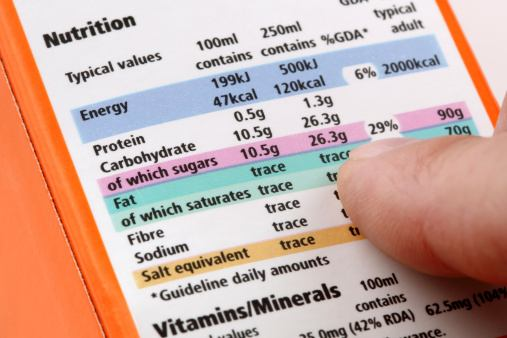
\includegraphics[scale=0.5]{immagini/etichetta}
%			\caption{Informazioni di un prodotto (\url{goo.gl/pxeYU1}).}
%		\end{figure}
%		
%		Questi dati sono utilizzati in molti ambiti, come ad esempio:
%		\begin{itemize}
%			\item La stampa dell'etichetta da apporre sulla confezione di un prodotto.
%			\item La categorizzazione di tipologie di prodotto sugli scaffali di un supermercato o sul sito di un \textit{e-commerce}.
%			\item L'identificazione e la ricerca di prodotti con particolari caratteristiche.
%			\item La gestione di magazzino.
%			\item L'identificazione di allergeni o particolari agenti chimici.
%			\item La raccolta di dati statistici e la generazione di reportistica.
%		\end{itemize}
%		
%		Dati i molti utilizzi, la memorizzazione delle informazioni è una necessità che negli anni ha avuto varie soluzioni e implementazioni.
%						
%		Attualmente IBC utilizza un \textit{database} relazionale per la persistenza dei dati. Questo porta al problema principale che il progetto offerto deve risolvere. Data la natura stessa del modello relazionale, è necessario definire una struttura prima di poter memorizzare un qualsiasi elemento. Gli attributi dei prodotti però sono variabili e non è raro trovare due prodotti appartenenti alla stessa categoria con qualche attributo non in comune.
%		
%		Un altro fattore da considerare è il fattore umano: dato che le informazioni dei prodotti vengono spesso fornite a IBC da personale non tecnico, capita a volte che gli attributi non rispettino i limiti imposti dalla struttura relazionale, portando all'impiego di risorse per riprogettare la struttura o tradurre gli attributi in un modello valido.
%		
%		Tenendo conto dei due punti appena esposti, l'attuale soluzione adottata dall'azienda prevede la definizione di una struttura che contempli tutti i possibili attributi di ogni categoria di prodotto. Le particolari istanze di ogni prodotto che non riportano un qualche attributo avranno il valore di quest'ultimo impostato a \texttt{null}.
%		
%		Questa soluzione è però poco logica ed è imposta dal modello relazionale. Un \textit{Content Repository} fornisce un'alternativa senza lo svantaggio appena esposto.
%		
%		IBC era quindi alla ricerca di una soluzione flessibile, che permettesse l'aggiunta di prodotti aventi proprietà variabili, utilizzando il modello JCR. Il \textit{tutor} ha affermato che l'obiettivo del prototipo da realizzare era verificare se fosse possibile implementare una soluzione utilizzando la libreria \gls{jackrabbit}. Anche in base ai risultati da me ottenuti, l'azienda deciderà in futuro se intraprendere un progetto su più ampia scala per la realizzazione di un \textit{software} utilizzando questa tecnologia.
%		
%		
%		\subsection{Introduzione a JCR}
%		Date le mie scarse conoscenze del dominio del progetto, ho impiegato i primi giorni lavorativi per effettuare uno studio preliminare. Ho consultato principalmente risorse presenti \textit{online}, tra cui:
%		\begin{itemize}
%			\item \textit{Paper} \jquote{JCR or RDBMS: why, when, how?}, per comprendere le differenze tra Relational DataBase Management System (d'ora in poi RDBMS) e Java Content Repository (d'ora in poi JCR).
%			\item Articolo \jquote{What is Java Content Repository} (\url{https://goo.gl/8HWDRZ}), per avere una descrizione di base di JCR.
%			\item Standard \gls{jsr170} e \gls{jsr283}.
%		\end{itemize}
%		
%		I risultati delle mie ricerche sono contenuti all'interno di due documenti che ho prodotto per IBC:
%		\begin{itemize}
%			\item \textbf{Confronto tra RDBMS e JCR:} documento che racconta la storia di JCR e analizza le differenze tra il modello relazionale e il modello JCR.
%			\item \textbf{Struttura JCR e funzionamento Jackrabbit:} documento che, a partire dagli \textit{standard} precedentemente citati, fornisce una spiegazione delle principali API per l'accesso a JCR. Inoltre, date le funzionalità aggiuntive fornite da Jackrabbit, nella seconda parte del documento descrivo la struttura di Jackrabbit e il suo funzionamento nel dettaglio.
%		\end{itemize}
%		
%		Un \textit{Content Repository} è un modello utilizzato per la memorizzazione di qualsiasi tipo di dato. Gli \textit{standard} \gls{jsr170} e \gls{jsr283} definiscono le API per JCR.
%		
%		Le differenze tra il modello relazionale e il JCR possono essere suddivise in varie aree, come analizzato nel seguente \textit{paper}:
%		\url{https://goo.gl/ngzgKt}.
%		
%		\begin{figure}[H]
%			\centering
%			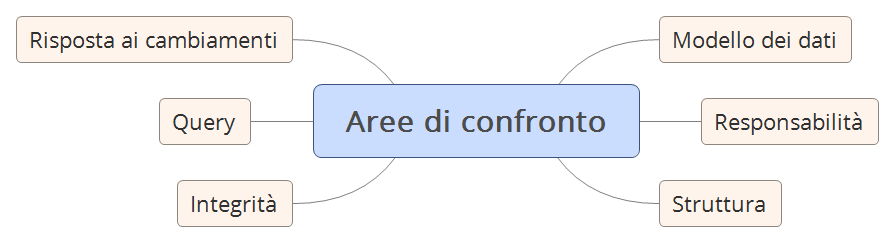
\includegraphics[scale=0.4]{immagini/aree-confronto}
%			\caption{Aree di confronto tra RDBMS e JCR.}
%		\end{figure}
%		
%		\begin{enumerate}
%			\item \textbf{Modello dei dati} \\
%			Con \jquote{modello dei dati} intendiamo il modo con cui i dati vengono organizzati, acceduti e messi in relazione tra di loro.
%			\paragraph{RDBMS} 
%			Il modello relazionale si basa sulla teoria degli insiemi e sulla definizione matematica di relazione, che ricordiamo essere un sottoinsieme del prodotto cartesiano tra \textit{n} insiemi. Dato che ognuno di questi dev'essere distinguibile dagli altri, ogni insieme è definito come dominio. Ad esempio, facendo riferimento alla tabella sottostante, i domini sono quello dei nomi (N), cognomi (C) ed età (E). 
%			
%			\begin{figure}[H]
%				\centering
%				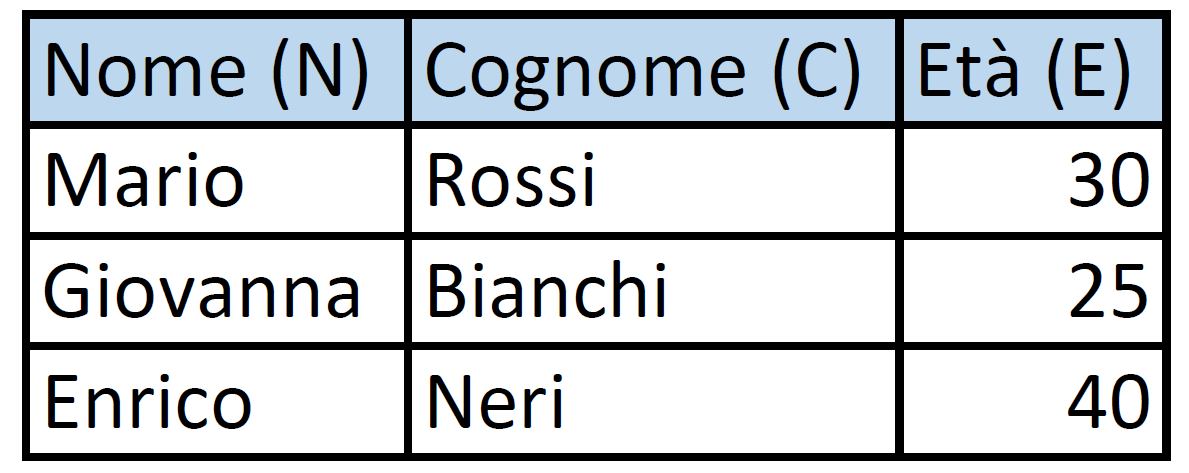
\includegraphics[scale=0.2]{immagini/modello-r}
%				\caption{Tabella che rappresenta una persona (\url{https://goo.gl/ngzgKt}).}
%			\end{figure}
%		
%			La definizione di relazione non implica la possibilità di creare associazioni tra le relazioni. Per fare questo, è necessario utilizzare l'algebra relazionale. 
%			
%			\paragraph{JCR} 
%			Il modello JCR si basa principalmente su una struttura ad albero, unendo le caratteristiche dei modelli gerarchici a quelle dei modelli a rete. Il risultato è una struttura ad albero che permette la connessione dei nodi orizzontalmente.
%			
%					\begin{figure}[H]
%						\centering
%						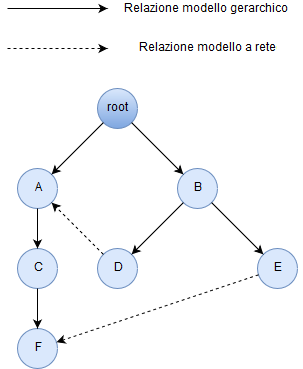
\includegraphics[scale=0.5]{immagini/modello-j}
%						\caption{Unione del modello a rete con il modello gerarchico (\url{https://goo.gl/ngzgKt}).}
%					\end{figure}
%				
%			\item \textbf{Responsabilità} \\
%			Quando si tratta di \textit{database} e persistenza dei dati, generalmente possono essere identificati tre ruoli principali:
%			\begin{itemize}
%				\item Il \textbf{\textit{database administrator} (DBA)}, che mantiene il \textit{database} in uno stato utilizzabile eseguendo attività di installazione, configurazione, \textit{backup} e \textit{data recovery}.
%				\item L'\textbf{\textit{application programmer}}, che scrive \textit{software} che accede al \textit{database}.
%				\item L'\textbf{utente}, che utilizza il \textit{software} per leggere, scrivere e modificare i dati nel \textit{database}.
%			\end{itemize}
%			I due modelli si differenziano anche sotto il punto di vista dei ruoli. Più precisamente, cambiano le responsabilità e i campi di interesse di ogni ruolo.
%			
%			
%			I campi di interesse presi in esame sono:
%			\begin{itemize}
%				\item \textbf{Contenuto}: tutti i dati inclusi nel \textit{database}.
%				\item \textbf{Struttura}: il modo con cui i dati sono suddivisi.
%				\item \textbf{Integrità}: lo stato di completezza dei dati.
%				\item \textbf{Coerenza}: la relazione ordinata, logica e consistente delle parti.
%			\end{itemize}
%			
%			
%			\paragraph{RDBMS} 
%				Nel modello relazionale generalmente è il DBA ad avere il controllo sulla struttura. L'\textit{application programmer} solitamente ha un qualche tipo di influenza sulle decisioni prese in questo campo, ma la decisione finale spetta al DBA. L'utente non ha alcuna responsabilità per quanto riguarda la struttura e può solo interagire con il \textit{database} tramite le operazioni fornite dal \textit{software}.
%				
%				\begin{figure}[H]
%					\centering
%					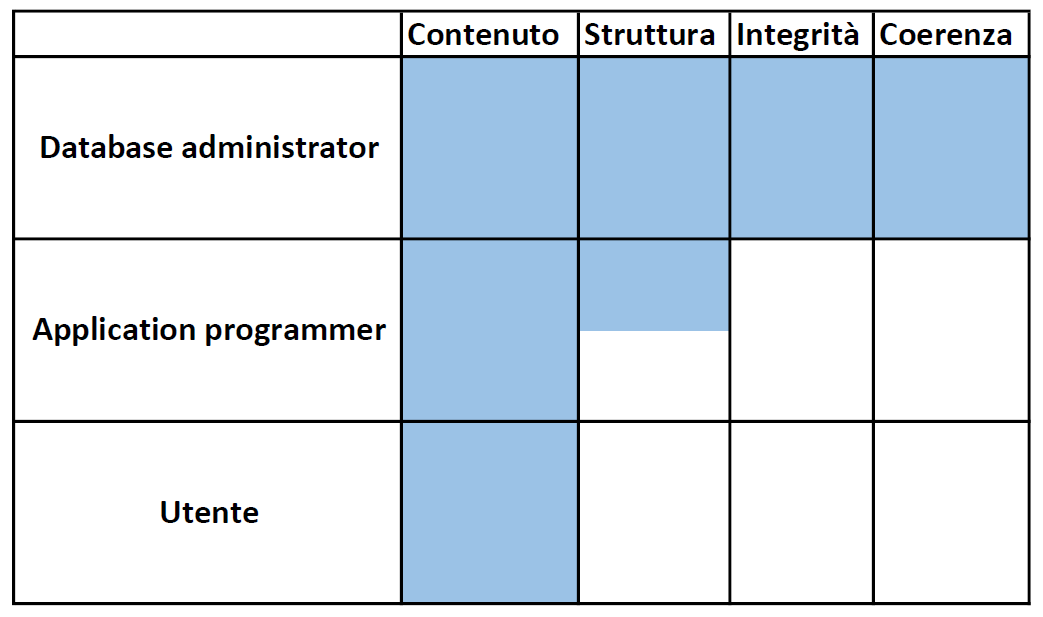
\includegraphics[scale=0.4]{immagini/ruoli-r}
%					\caption{Responsabilità dei ruoli in RDBMS (\url{https://goo.gl/ngzgKt}).}
%				\end{figure}
%			
%			
%			\paragraph{JCR} 
%				Nel modello JCR invece la struttura è responsabilità di tutti e tre i ruoli. Infatti, il controllo sulla struttura è più incentrato verso l'\textit{application programmer} e l'utente, riducendo di fatto le responsabilità del DBA in questo campo.
%				
%				
%				Uno dei vantaggi principali di questo approccio è che solitamente il ruolo di \textit{application programmer} è più vicino all'utente finale rispetto al DBA, quindi una collaborazione tra questi due ruoli per la definizione della struttura è solitamente più efficace.
%				
%				
%				È anche possibile costruire \textit{software} che permettono al solo utente finale di definire la struttura, aggiungendo attributi ai dati a tempo di esecuzione, sottostando ai vincoli definiti dal DBA e dall'\textit{application programmer}.
%				
%				\begin{figure}[H]
%					\centering
%					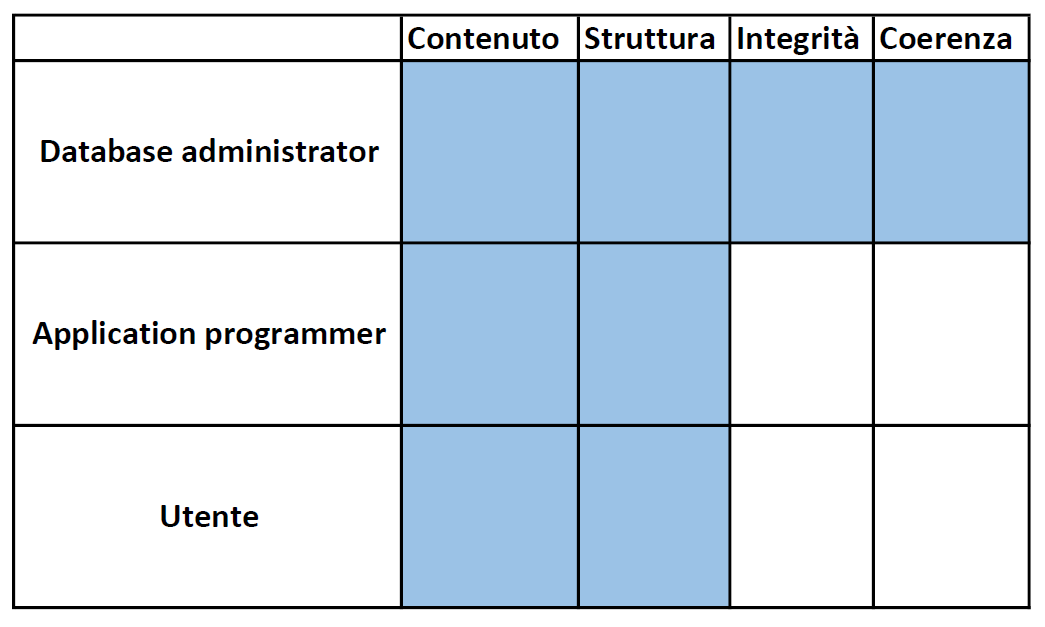
\includegraphics[scale=0.4]{immagini/ruoli-j}
%					\caption{Responsabilità dei ruoli in JCR (\url{https://goo.gl/ngzgKt}).}
%				\end{figure}
%				
%				\item \textbf{Struttura} \\
%					Con \jquote{struttura} intendiamo il modo con cui i dati sono suddivisi e a quali costrizioni essi sono sottoposti. 
%					
%					
%					Le differenze in termini di struttura rendono i due modelli diametralmente opposti, con vantaggi e svantaggi in entrambi gli approcci.
%					
%					\paragraph{RDBMS} 
%						Nel modello RDBMS, i dati sono guidati dalla struttura. Un dato, per essere istanziato, ha bisogno che la struttura sia completamente definita. Questo modello si basa sull'assunzione che dati e struttura siano sempre completamente separati e indipendenti, ma nella realtà quest'assunzione non è sempre valida. Come esposto precedentemente, ci sono casi d'uso in cui la struttura del dato cambia nel tempo, portando all'aggiunta di nuovi campi o ad un'intera riprogettazione nei casi più sfortunati.
%					
%					\paragraph{JCR} 
%						In JCR non è richiesta la definizione di alcuna struttura per istanziare i dati. Nodi, attributi e valori possono essere creati senza nessun prerequisito. Infatti, la struttura emerge con l'inserimento dei dati. Con il modello JCR non è più necessario definire tutti i possibili attributi al momento della creazione di un tipo di dato, garantendo una maggiore flessibilità ed estendibilità.
%						
%				
%				
%				\item \textbf{Integrità} \\
%					L'integrità di un \textit{database} indica l'impossibilità di distruzioni e alterazioni dei dati, siano esse accidentali o intenzionali. Questa caratteristica è implementata in diversi modi a seconda del modello.
%					
%					\paragraph{RDBMS} 
%						Il modello relazionale adotta una strategia simile ad una \textit{white list}, ovvero i dati possono essere salvati solo se è definita una struttura. È quindi quest'ultima che garantisce buona parte dell'integrità, ad esempio attraverso i vincoli di dominio.
%					
%					
%					\paragraph{JCR} 
%						In opposizione al modello RDBMS, JCR si basa su un approccio a \textit{black list}. Un nodo generico del \textit{Content Repository} può avere qualunque nodo figlio e qualsiasi proprietà, senza vincoli su tipi e valori.
%						
%						
%						Eventuali vincoli possono essere imposti assegnando ai nodi dei tipi. Un tipo di nodo descrive vincoli sul tipo dei nodi figli o sui valori delle proprietà che il nodo stesso può avere. Assegnando un tipo anche ai nodi figli e continuando a procedere in questo modo è possibile imporre sempre più limiti alla struttura.
%						
%				\item \textbf{\textit{Query}} \\
%					Anche il tipo e la potenza delle \textit{query} differenzia i due modelli.
%				
%					\paragraph{RDBMS} 
%						Data la definizione di relazione, il modello RDBMS si basa sull'algebra relazionale per la definizioni delle operazioni di base. Il vantaggio di questo modello è che sia l'\textit{input} che l'\textit{output} delle operazioni sono relazioni. È quindi possibile concatenare espressioni complesse senza troppe difficoltà. Inoltre, la maggior parte dei linguaggi di \textit{query} fornisce anche la possibilità di effettuare cambiamenti sequenziali al risultato di una \textit{query}.
%					
%					
%					\paragraph{JCR} 
%						Nel JCR è necessario utilizzare un modello di \textit{query} astratto per effettuare operazioni. Questo modello astratto serve a mappare il modello JCR con le nozioni di relazione, domini, tuple e attributi tipiche del modello relazionale.
%						
%						
%						Uno dei principali svantaggi è che, con l'implementazione JCR di \textit{default}, non è possibile effettuare cambiamenti sequenziali con una \textit{query}.
%					
%					
%						Nel complesso, JCR offre un supporto più limitato rispetto al modello relazionale per quanto riguarda le \textit{query}, ma ha vantaggi prestazionali nell'esecuzione di ricerche \gls{fulltext}.
%					
%				\item \textbf{Risposta ai cambiamenti} \\
%					Nonostante un'analisi dei requisiti svolta in maniera impeccabile, è possibile che nuovi requisiti emergano dopo che l'architettura di un sistema è già stata definita. Un modello di sviluppo non strettamente sequenziale, come ad esempio quello incrementale, permette solitamente di soddisfare i nuovi requisiti senza dover riprogettare interamente il sistema. Tuttavia, un impatto a livello di architettura è spesso inevitabile e comporta dei costi. Per diminuire questi costi, è preferibile adottare un modello dei dati che riesca ad accettare i cambiamenti in maniera trasparente.
%					
%					\paragraph{RDBMS} 
%						Nel modello relazionale, quasi tutti i cambiamenti architetturali richiedono un cambiamento a livello di logica dei dati. Questo modello non è quindi molto adatto a casi in cui sono necessari molti cambiamenti.
%					
%					
%					\paragraph{JCR} 
%						Dato che un'architettura basata sul modello JCR è molto lasca, è possibile aggiungere nuovi campi dati (e quindi soddisfare i requisiti che lo richiedono) senza modificare il livello di logica dei dati. Con JCR si ha quindi un disaccoppiamento molto forte tra dati e logica dell'applicazione. 
%						Data questa caratteristica, l'aggiunta di eventuali campi dati impatterà solo il livello di logica dell'applicazione e di interfaccia. Alcuni \gls{framework} si occupano di un ulteriore disaccoppiamento tra logica e interfaccia operando in maniera simile. Questa combinazione genera un sistema che risponde ai cambiamenti in modo estremamente dinamico e con costi contenuti.
%		\end{enumerate}
%				
%
%		
%	\subsection{Obiettivi}
%		\label{sec:obiettivi}
%	
%	Dopo vari incontri con il \textit{tutor} aziendale, abbiamo definito gli obiettivi da raggiungere, suddividendoli in obbligatori, desiderabili e facoltativi.
%	
%	
%	A grandi linee, nelle trecentoventi ore previste dallo \textit{stage} l'azienda si aspettava:
%	\begin{itemize}
%		\item Uno studio e la produzione di documentazione sulle differenze tra \textit{database} relazionale e \textit{Content Repository}.
%		\item Uno studio e la produzione di documentazione sugli \textit{standard} JSR 170 e JSR 283, rispettivamente Java Content Repository 1.0 e 2.0.
%		\item La produzione di esempi di codice sorgente riguardanti l'utilizzo della libreria \gls{jackrabbit}.
%		\item La realizzazione di un prototipo che permettesse operazioni di aggiunta, visualizzazione, modifica e rimozione di prodotti commerciali e dei loro attributi
%	\end{itemize}
%
%	Con il \textit{tutor} abbiamo discusso anche dell'eventuale possibilità dello studio e dell'implementazione di soluzioni distribuite, ma dato il tempo limitato a disposizione e la corposità delle librerie da apprendere abbiamo deciso di non inserire questa richiesta negli obiettivi.
%	
%	
%	A seguire includo una lista dettagliata degli obiettivi suddivisi per importanza.
%	
%	\begin{table}[H]
%		\begin{tabularx}{\textwidth}{| X |}
%			\Xhline{2\arrayrulewidth}
%			\textbf{Obiettivi obbligatori} \\
%			\Xhline{2\arrayrulewidth}
%			Studio e documentazione sulle differenze tra \textit{database} relazionale e \textit{Content Repository} \\
%			\hline
%			Studio e documentazione sulla storia di \textit{Content Repository} \\
%			\hline
%			Studio di JSR 170 e JSR283: Content Repository for Java (JCR), con produzione di codice e documentazione \\
%			\hline
%			Studio e documentazione della struttura di JCR \\
%			\hline
%			Studio e documentazione della definizione di nodo \\
%			\hline
%			Studio e documentazione riguardo aggiunta, rimozione e modifica di proprietà di un nodo \\
%			\hline
%			Studio e documentazione riguardo l'aggiunta e la rimozione di tipologie di nodo \\
%			\hline
%			Studio e documentazione riguardo la referenziazione di elementi \\
%			\hline
%			Studio e documentazione riguardo l'esecuzione di \textit{query} utilizzando XPath e JCR-SQL2 \\
%			\hline
%			Studio e documentazione riguardo l'indicizzazione \\
%			\hline
%			Progettazione di un prototipo di applicazione che gestisca le informazioni di prodotti commerciali \\
%			\hline
%			Realizzazione di un prototipo di applicazione che gestisca le informazioni di prodotti commerciali \\
%			\Xhline{2\arrayrulewidth}
%			\textbf{Obiettivi desiderabili} \\
%			\Xhline{2\arrayrulewidth}
%			Realizzazione della \gls{gui} del prototipo \\
%			\Xhline{2\arrayrulewidth}
%			\textbf{Obiettivi facoltativi} \\
%			\Xhline{2\arrayrulewidth}
%			Studio e documentazione riguardo i \textit{workspace} multipli \\
%			\hline
%		\end{tabularx}
%		\caption{Obiettivi del progetto}
%	\end{table}
%	
%	\subsection{Vincoli}
%		\begin{figure}[H]
%		\centering
%			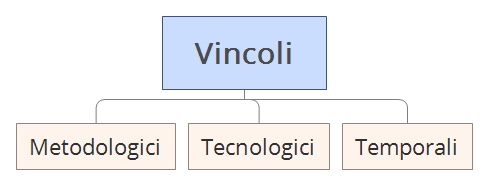
\includegraphics[scale=0.5]{immagini/vincoli}
%			\caption{Vincoli del progetto}
%		\end{figure}
%	
%	\subsubsection*{Metodologici}
%		La prima tipologia di vincoli a cui il progetto era sottoposto erano i vincoli metodologici.
%		
%		
%		Con il \textit{tutor} aziendale abbiamo stabilito che il lavoro doveva essere svolto presso la sede aziendale, per avere miglior approccio e comunicazione con il \textit{tutor} stesso e gli altri colleghi. L'azienda ha posto questo vincolo anche per cercare raggiungere l'obiettivo di prospettiva di assunzione descritto nella sezione \ref{sec:motivazioni_aziendali}.
%		
%		
%		Un altro vincolo stabilito riguardava l'interazione con il \textit{tutor} e la richiesta di informazioni tecniche ai colleghi. Dati i frequenti impegni del \textit{tutor}, nel caso di necessità di informazioni tecniche avrei dovuto chiedere ai colleghi d'ufficio facenti parte del \textit{team} Java 3, senza però abusare di tale possibilità. Uno degli obiettivi che l'azienda ha cercato di raggiungere con questo vincolo è quello di migliorare le mie capacità di \textit{problem solving} e di lavoro in autonomia, insegnandomi a riconoscere i problemi risolvibili da me e quelli che invece necessitano di personale più esperto. I rapporti con il \textit{tutor} si sarebbero dovuti limitare a richieste riguardo i requisiti e a revisioni periodiche per valutare i risultati raggiunti.
%		
%	\subsubsection*{Tecnologici}
%		\label{sec:vincoli-tecnologici}
%		Gli unici vincoli tecnologici imposti dall'azienda riguardavano l'implementazione di esempi di codice e di un prototipo basato sulla libreria Jackrabbit, utilizzando quindi il linguaggio Java.
%		
%		
%		Per quanto riguarda il versionamento, IBC ha predisposto un \textit{repository} SVN su cui avrei dovuto effettuare i \textit{commit} di codice e documentazione.
%		
%		
%		Non abbiamo fissato vincoli stretti riguardo la gestione della configurazione, anche se il \textit{tutor} mi ha fortemente consigliato di utilizzare Maven, data l'esperienza positiva che l'azienda ha avuto con tale strumento.
%		
%		
%		La scelta di eventuali \textit{framework} per l'implementazione dell'interfaccia grafica del prototipo era libera, a patto che fosse possibile l'interfacciamento con il JCR offerto da Jackrabbit. Questo mi ha portato a dover effettuare una scelta:
%		\begin{itemize}
%			\item La prima opzione che ho considerato è stato l'utilizzo del linguaggio PHP, da me già conosciuto. Ho presto realizzato che per percorrere questa strada avrei dovuto utilizzare la libreria Jackalope, che fornisce un'implementazione di JCR accessibile tramite API PHP. Nonostante la presenza di Jackalope-Jackrabbit, un'implementazione basata sul JCR fornito da \gls{jackrabbit}, ho trovato questa soluzione troppo complicata e scarsamente documentata.
%			\item La seconda opzione che ho considerato è stato JavaServer Faces (JSF), un \textit{framework} Java basato sul \textit{design pattern} MVC per lo sviluppo di applicazioni \textit{web}. Dopo aver letto varie opinioni \textit{online}, ho scartato questa scelta in quanto risulta essere molto complicata. Uno dei motivi principali di questa complessità è, come citato da ThoughtWorks nell'articolo raggiungibile al link \url{https://goo.gl/dfxpaC}, \jquote{pensiamo che [JSF] sia imperfetto in quanto tenta di astrarre troppo l'HTML, il CSS e l'HTTP}.
%			\item La terza opzione, quella da me scelta, è stato Apache Wicket, anch'esso un \textit{framework} Java che utilizza MVC con la caratteristica aggiuntiva di essere basato su componenti. Questa caratteristica, unita al fatto che Wicket permetteva l'interfacciamento senza alcuna complicazione al JCR e che era utilizzato anche da IBC, mi hanno portato a preferirlo alle altre tecnologie.
%		\end{itemize}
%		Alla luce di questa e altre decisioni, includo una tabella che elenca le tecnologie utilizzate durante il progetto.
%		
%		\begin{table}[H]
%			\centering
%			\begin{tabularx}{\textwidth}{|X | X | X |}
%				\hline
%				\rowcolor{lightgray}
%			  \textbf{Documentazione} & 	\textbf{{Config.} e \mbox{versionamento}}  &  \textbf{Sviluppo} \\
%				\hline
%				 LibreOffice & Maven & Eclipse \\
%				\hline
%				 & SVN & Jackrabbit \\
%				\hline
%				 & Tomcat & Wicket \\
%				\hline
%				& & Wicket-Bootstrap \\
%				\hline
%				& & JUnit \\
%				\hline
%			\end{tabularx}
%			\caption{Principali tecnologie utilizzate nel progetto.}
%		\end{table}
%	
%	\subsubsection*{Temporali}
%		Per quanto riguarda i vincoli temporali, gli orari di lavoro erano gli stessi del personale IBC, ovvero dal Lunedì al Venerdì con orario dalle 8:30 alle 12:30 e dalle 14:00 alle 18:00. L'azienda non ha richiesto moduli o procedure particolari per l'assenza da lavoro o la variazione di orario per motivi universitari, tranne la comunicazione a voce al \textit{tutor} o ad un collega.
%		
%		
%	\subsection{Pianificazione del lavoro}
%		La pianificazione del lavoro ha dovuto tener conto dei vincoli temporali esposti nella sezione precedente.
%		
%		
%		Ho pianificato lo svolgimento delle attività in otto settimane lavorative da quaranta ore ciascuna, come mostrato nel Gantt sottostante.
%			\begin{figure}[H]
%				\centering
%				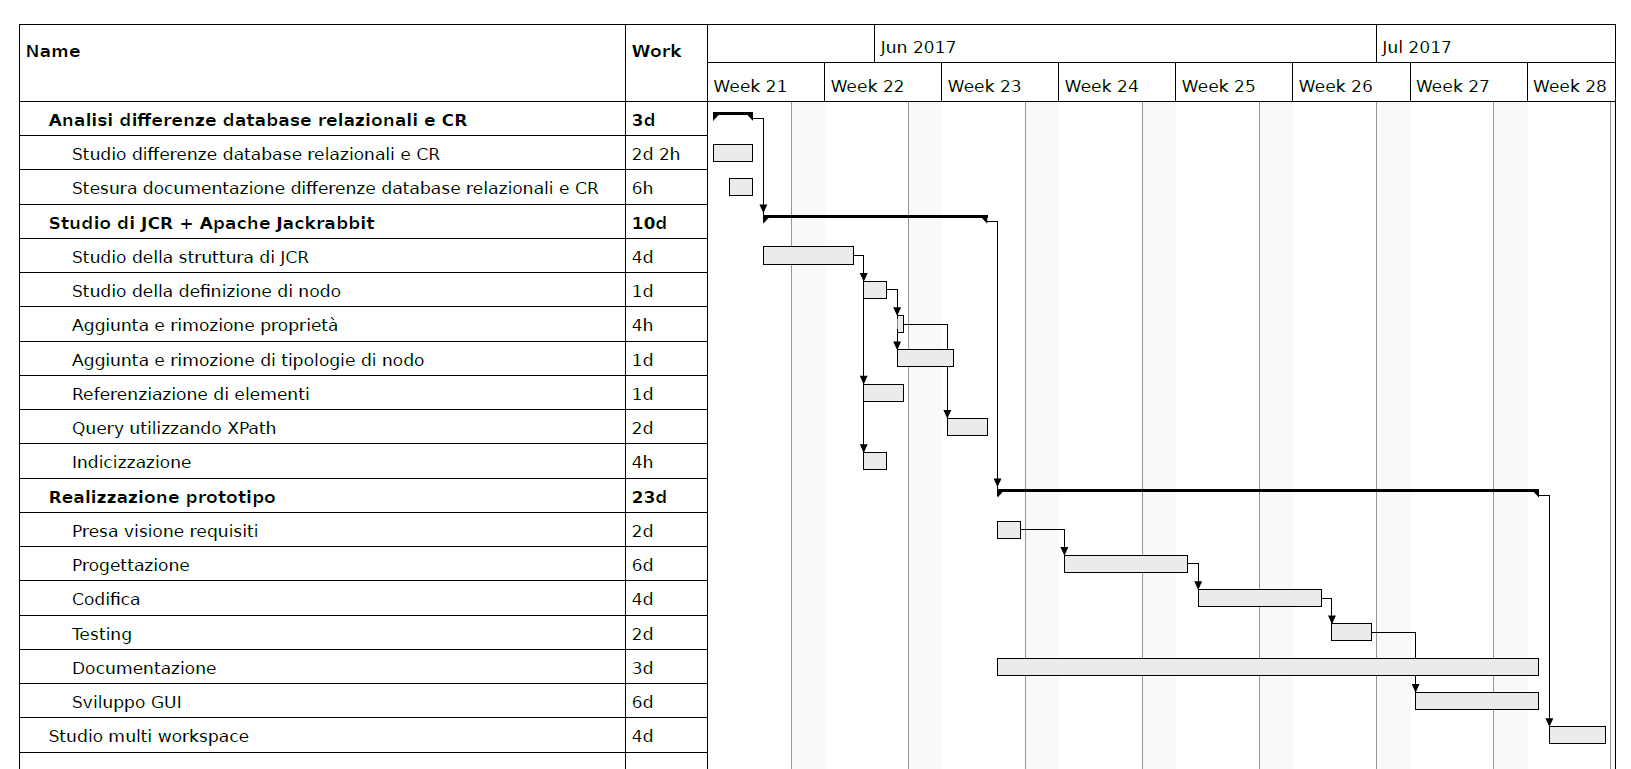
\includegraphics[width=\textwidth]{immagini/gantt-pianificazione}
%				\caption{Pianificazione temporale.}
%			\end{figure}
%		
%		Durante lo svolgimento iniziale delle attività di analisi e studio ho seguito il piano, ma durante la realizzazione del prototipo non ho rispettato la netta sequenzialità tra realizzazione del prototipo e sviluppo della GUI. Il motivo di questa decisione è dovuto al fatto che ho deciso di raggiungere l'obiettivo desiderabile stabilito dal piano di lavoro. Ho avuto quindi la necessità di iniziare ad apprendere il \textit{framework} scelto per l'interfaccia al più presto, portandomi a svolgere le attività di realizzazione della logica del prototipo e della parte grafica in parallelo.
%
%		Tenendo conto di questo punto, il reale svolgimento delle attività è stato il seguente.
%		
%		\begin{figure}[H]
%			\centering
%			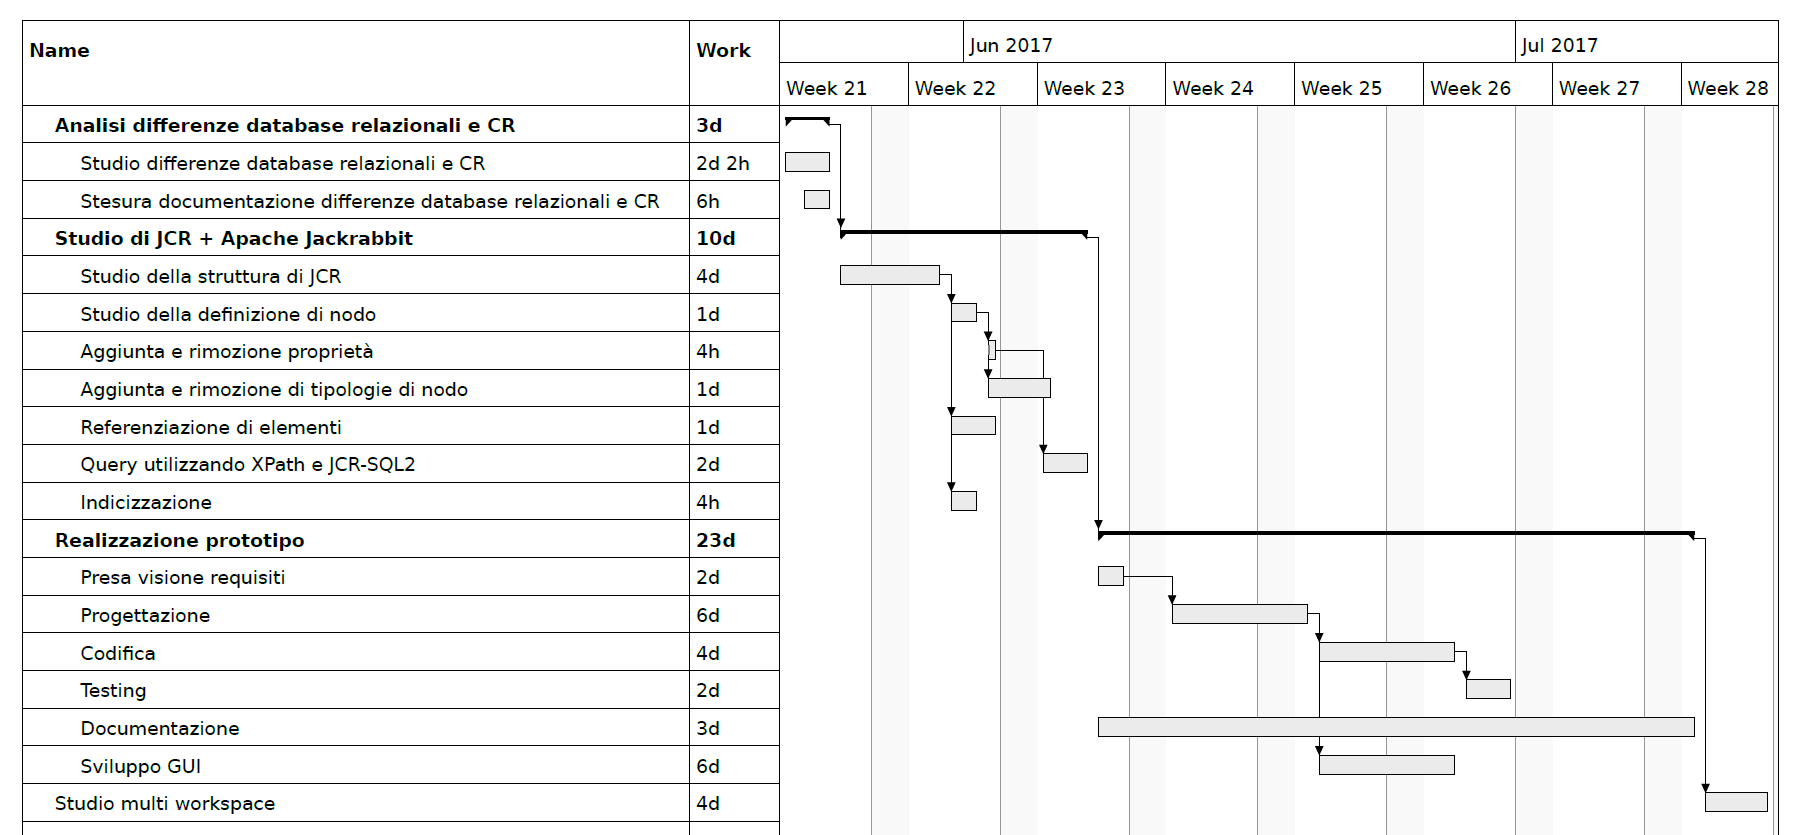
\includegraphics[width=\textwidth]{immagini/gantt-consuntivo}
%			\caption{Svolgimento attività.}
%		\end{figure}
%		
%
%\section{\textit{Stage} in IBC: motivazioni personali}
%	\label{sec:motivazioni_personali}
%	Durante la partecipazione a StageIt ho sostenuto colloqui con undici aziende. La mia scelta è ricaduta su IBC per una serie di motivi suddivisibili in tre tipologie: economici e logistici, professionali, personali.
%	
%	\subsubsection*{Economici e logistici}
%		\begin{itemize}
%			\item L'azienda, al contrario di molte altre, offriva un rimborso spese. Personalmente lo considero come un modo di riconoscere del valore nel lavoro svolto dallo stagista. Inoltre, la gratificazione ricevuta da questo riconoscimento è un buon punto di partenza per un rapporto che potrebbe continuare dopo la fine dello \textit{stage}.
%			\item Il posizionamento del luogo di lavoro, situato a dieci minuti da casa e vicino a Padova, era ideale per permettermi di raggiungere in breve tempo la sede dell'università. Infatti, data la necessità di terminare il progetto didattico di \gls{swe}, ho dovuto presenziare ad alcuni incontri con i miei compagni di progetto dopo l'orario di lavoro. Un'azienda situata più lontano non mi avrebbe permesso tale flessibilità.
%		\end{itemize}
%	
%	\subsubsection*{Professionali}
%		\begin{itemize}
%			\item IBC è un'azienda che non si occupa solamente di consulenza, ma produce anche \textit{software} proprio. Svolgere lo \textit{stage} presso IBC mi ha permesso di essere immerso in un ambiente che unisce entrambe le realtà.
%			\item Data la diffusione del linguaggio Java in ambito aziendale, ho valutato positivamente un'esperienza in una realtà che, oltre ad usare tale linguaggio, produce applicazioni che si basano su \gls{javaee}.
%		\end{itemize}
%	
%	\subsubsection*{Personali}
%	\begin{itemize}
%		\item Con questo \textit{stage} ho voluto valutare se l'impiego presso un'azienda che produce \textit{software} fosse adatto a me. Inoltre, dato che questa sarebbe stata la mia prima esperienza lavorativa, mi sono posto come obiettivo quello di rapportarmi con il personale esperto per avere consigli ed informazioni su come gestire un lavoro in campo informatico.
%	\end{itemize}
%
%%**************************************************************
%%\chapter{L'azienda}
%%\label{cap:lazienda}
%%%**************************************************************
%%
%%Introduzione al contesto applicativo.\\
%%
%%\noindent Esempio di utilizzo di un termine nel glossario \\
%%\gls{api}. \\
%%
%%\noindent Esempio di citazione in linea \\
%%\cite{site:agile-manifesto}. \\
%%
%%\noindent Esempio di citazione nel pie' di pagina \\
%%citazione\footcite{womak:lean-thinking} \\
%%
%%%**************************************************************
%%\section{L'azienda}
%%
%%Descrizione dell'azienda.
%%
%%%**************************************************************
%%\section{L'idea}
%%
%%Introduzione all'idea dello stage.
%%
%%%**************************************************************
%%\section{Organizzazione del testo}
%%
%%\begin{description}
%%    \item[{\hyperref[cap:processi-metodologie]{Il secondo capitolo}}] descrive ...
%%    
%%    \item[{\hyperref[cap:descrizione-stage]{Il terzo capitolo}}] approfondisce ...
%%    
%%    \item[{\hyperref[cap:analisi-requisiti]{Il quarto capitolo}}] approfondisce ...
%%    
%%    \item[{\hyperref[cap:progettazione-codifica]{Il quinto capitolo}}] approfondisce ...
%%    
%%    \item[{\hyperref[cap:verifica-validazione]{Il sesto capitolo}}] approfondisce ...
%%    
%%    \item[{\hyperref[cap:conclusioni]{Nel settimo capitolo}}] descrive ...
%%\end{description}
%%
%%Riguardo la stesura del testo, relativamente al documento sono state adottate le seguenti convenzioni tipografiche:
%%\begin{itemize}
%%	\item gli acronimi, le abbreviazioni e i termini ambigui o di uso non comune menzionati vengono definiti nel glossario, situato alla fine del presente documento;
%%	\item per la prima occorrenza dei termini riportati nel glossario viene utilizzata la seguente nomenclatura: \emph{parola}\glsfirstoccur;
%%	\item i termini in lingua straniera o facenti parti del gergo tecnico sono evidenziati con il carattere \emph{corsivo}.
%%\end{itemize}           
%% !TEX encoding = UTF-8
% !TEX TS-program = pdflatex
% !TEX root = ../tesi.tex


\chapter{Tools and applications}
	\section{Network Simulator 3}
	Network Simulator 3 (ns-3) is a discrete-event network simulator for Internet systems, targeted primarily for research and educational use. ns-3 is free software, licensed under the GNU GPLv2 license, and is publicly available for research, development, and use.
	
	
	ns-3 development began in 2006 by a team lead by Tom Henderson, George Riley, Sally Floyd and Sumit Roy. Its first version was released on June 30, 2008. 
	
	
	ns-3 is the successor of ns-2, released in 1989. The fact that the former was built from scratch makes it impossible to have backward compatibility. In fact, ns-2 used oTCL scripting language to describe network topologies and C++ to write the core of the simulation. This choice was due to avoid the very time consuming C++ code recompilation, exploiting the interpreted language oTCL. ns-2 mixed the \jquote{fast to run, slow to change} C++ with the \jquote{slow to run, fast to change} oTCL language. Since compilation time was not an issue with modern computing capabilities, ns-3 developers chose to utilize exclusively C++ code (and optional Python bindings) to develop simulations.
	
	\subsection{Modules and module structure}
	ns-3 is composed of various modules, which are groups of classes, examples and tests each related to a certain feature. The components of a module work in a cohesive way in order to offer APIs to other modules and users. Some examples of built-in modules are:
	\begin{itemize}
		\item WiFi;
		\item AODV; 
		\item CSMA.
	\end{itemize}
	The obstacle shadowing propagation loss model and the Fast Broadcast algorithm have been implemented as modules too.
	
	
	Modules follow a prototypical structure in order to promote clarity and offer built-in documentation. \imgrefcap{fig:ns-3-module} shows the typical module structure.
	
	\begin{figure}[H]
		\centering
		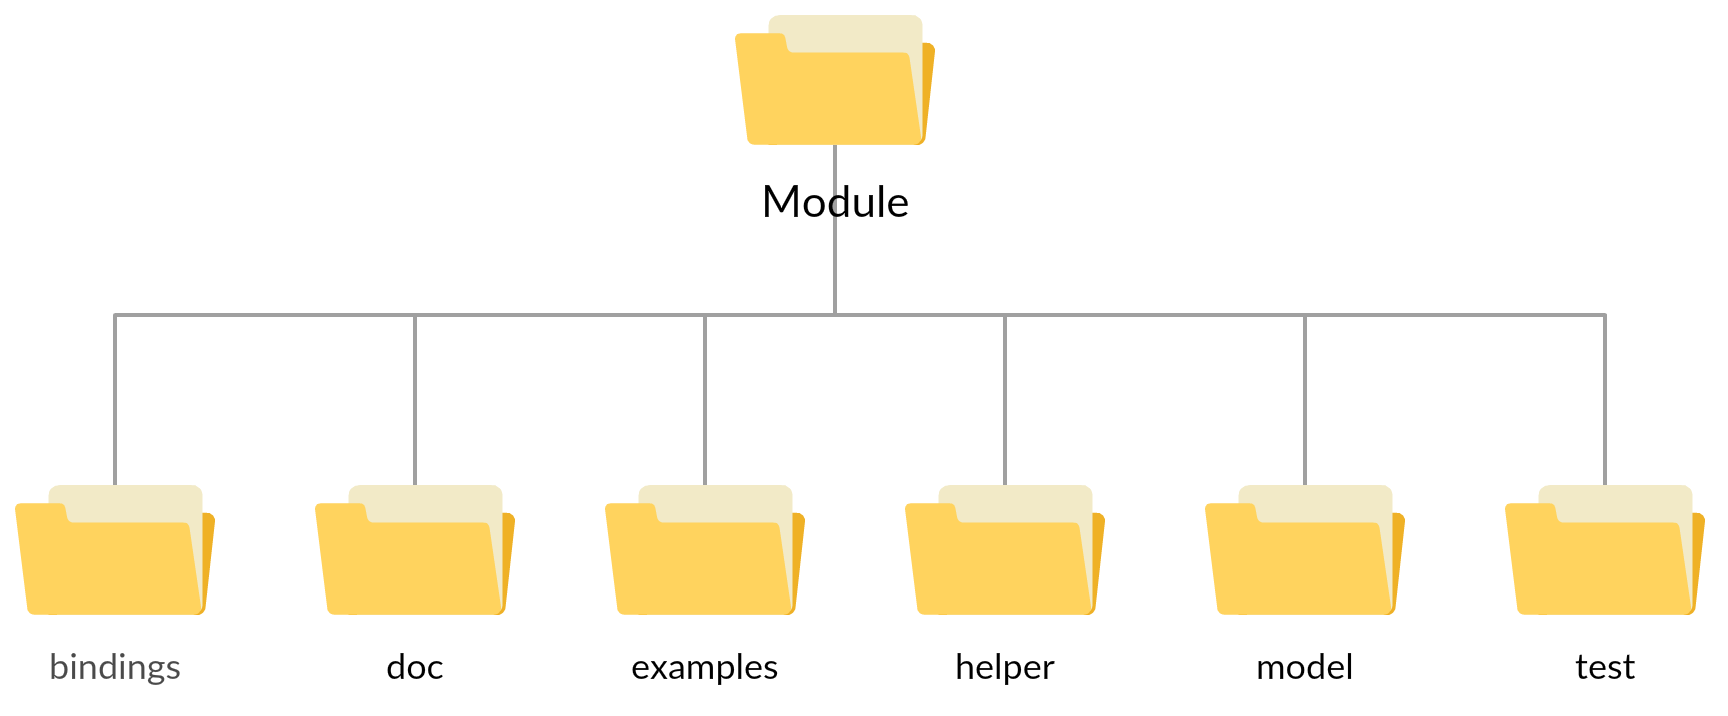
\includegraphics[width=\textwidth]{immagini/ns-3-module}
		\caption{ns-3 module structure}
		\label{fig:ns-3-module}
	\end{figure}
	
	The following directories can be found inside a module's root directory:
	\begin{itemize}
		\item \textbf{bindings:} Python bindings used to make the module's API compatible with Python;
		\item \textbf{doc:} documentation of the module;
		\item \textbf{examples:} examples and proof of concepts of what can be done using the module;
		\item \textbf{helper:} higher level APIs to make the module easier to use;
		\item \textbf{model:} headers and source files which implement the module's logic; 
		\item \textbf{test:} test suite and test cases to test the module.
	\end{itemize}
	
	\subsection{Key elements}
	The element at the base of ns-3 is called \textit{node}, instance of \texttt{ns3::Node}. A node can be thought of as a shell of a computer. Various other elements can be added to nodes, such as:
	\begin{itemize}
		\item NetDevices (e.g. \acrshort{nica}s, which enable nodes to communicate over \textit{channels};
		\item protocols;
		\item applications. 
	\end{itemize}
	It is the last those which implement the logic of a simulation. For example, the \texttt{UdoEchoClientApplication} and \texttt{UdpEchoServerApplication} can be used to implement a client/server application which exchange and print the packets' content over the network. The Fast Broadcast protocol has been implemented as an application as well.
	
	
	The \textit{channels} model various type of transmission media, such as the wired and the wireless ones.
	
	\subsection{Structure of a simulation}
	A simulation can be implemented in many ways, but in most cases the following steps are executed:
	\begin{itemize}
		\item manage command line arguments (e.g. number of nodes to consider in the simulation, transmission range, etc.);
		\item initialize all the necessary fields in classes;
		\item create nodes;
		\item set up physical and MAC layers;
		\item set up link layer, routing protocols and addresses;
		\item configure and install applications on nodes;
		\item position nodes and (optionally) give them a mobility model;
		\item schedule user defined events, such as transmissions of packets;
		\item start the simulation;
		\item collect and manage output data.
	\end{itemize}
	
	\subsection{NetAnim}
	Netanim is an offline animator tool based on the Qt toolkit. It collects an XML tracefile during the execution of a simulation and can be used to animate the simulation, analyzing packet transmissions and contents.
	
	\begin{figure}[H]
		\centering
		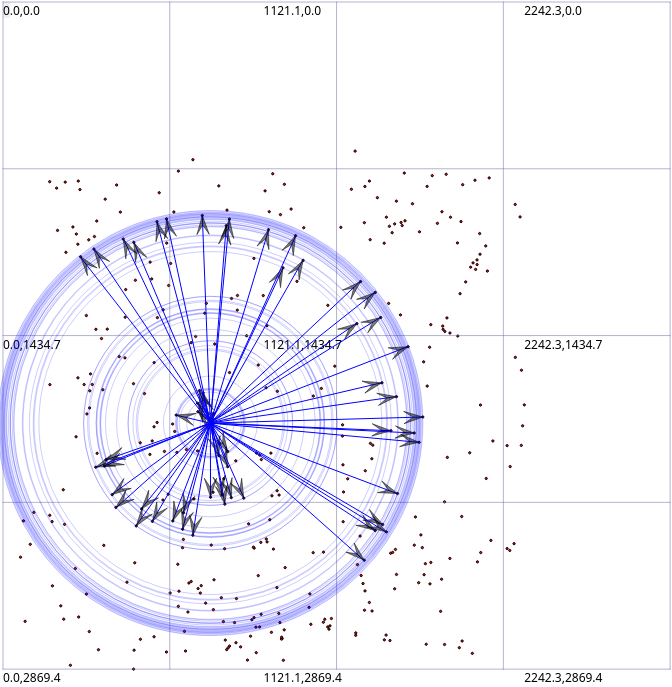
\includegraphics[scale=0.38]{immagini/netanim}
		\caption{Packet transmission in NetAnim}
		\label{fig:netanim}
	\end{figure}
	
	\section{Simulation of Urban MObility}
	Simulation of Urban MObility is an open-source road traffic simulation package. It is written in C++ and licensed under GPLv3. 
	
	
	It offers different tools to analyze and manage real maps from the urban mobility point of view, including pedestrian movement and various types of vehicles.
	
	
	The original work \cite{ROM2017} utilized SUMO to produce, starting from real maps obtained from OpenStreetMap (OSM), two files:
	\begin{enumerate}
		\item a \texttt{.poly} file using the SUMO tool \textit{Polyconvert}. This file contains information about all the obstacles, such as buildings, useful for the Obstacle Shadowing module;
		\item a \texttt{.ns2mobility} file using the SUMO tool \textit{TraceExporter}. This file contains information about the vehicles and their positioning. 
	\end{enumerate}
	The process of generating these two files necessary for ns-3 simulations requires some intermediate steps. The full process is represented in \imgref{fig:sumo-process}. 
	
	The original work considered a only a distance of 25 meters between vehicles; this work considers various distances, ranging from 15 to 45 meters. \imgrefcap{fig:sumo-distances}  shows the same scenario (Padua) with different distances between vehicles.
	
	\begin{figure}[H]
		\centering
		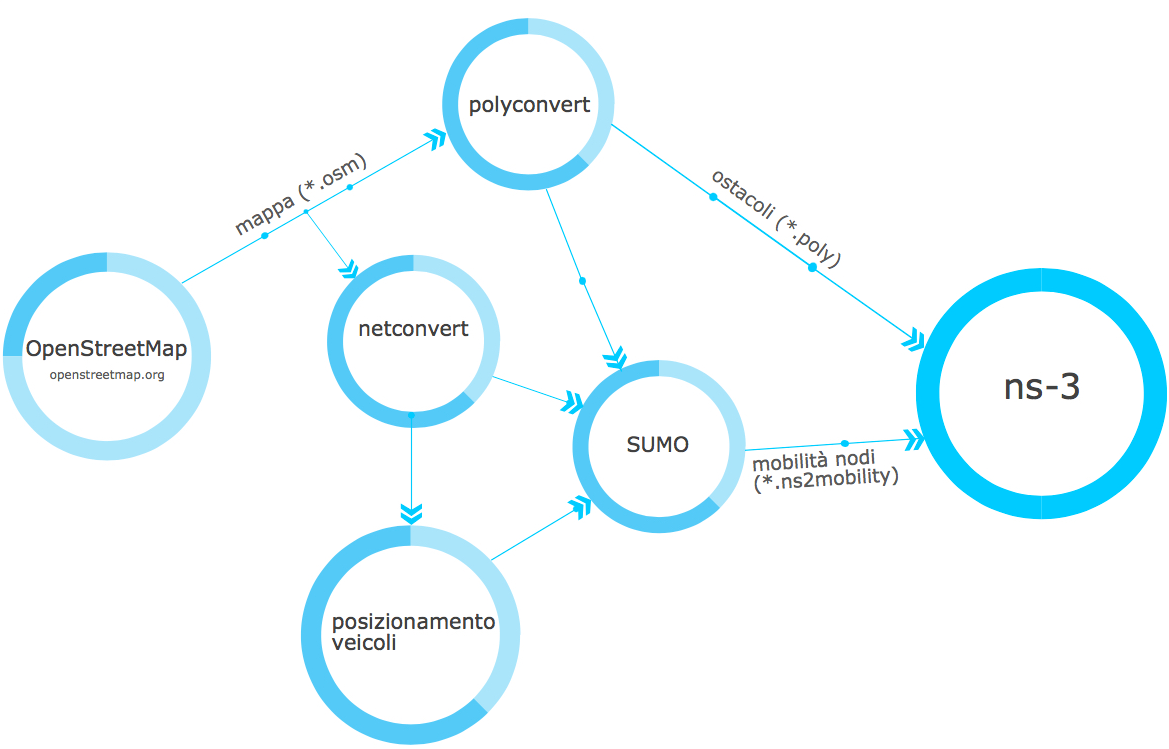
\includegraphics[width=\textwidth]{immagini/sumo-process}
		\caption{Steps to generate necessary files using SUMO (\cite{ROM2017})}
		\label{fig:sumo-process}
	\end{figure}
	
	\begin{figure}[H]
		\centering
		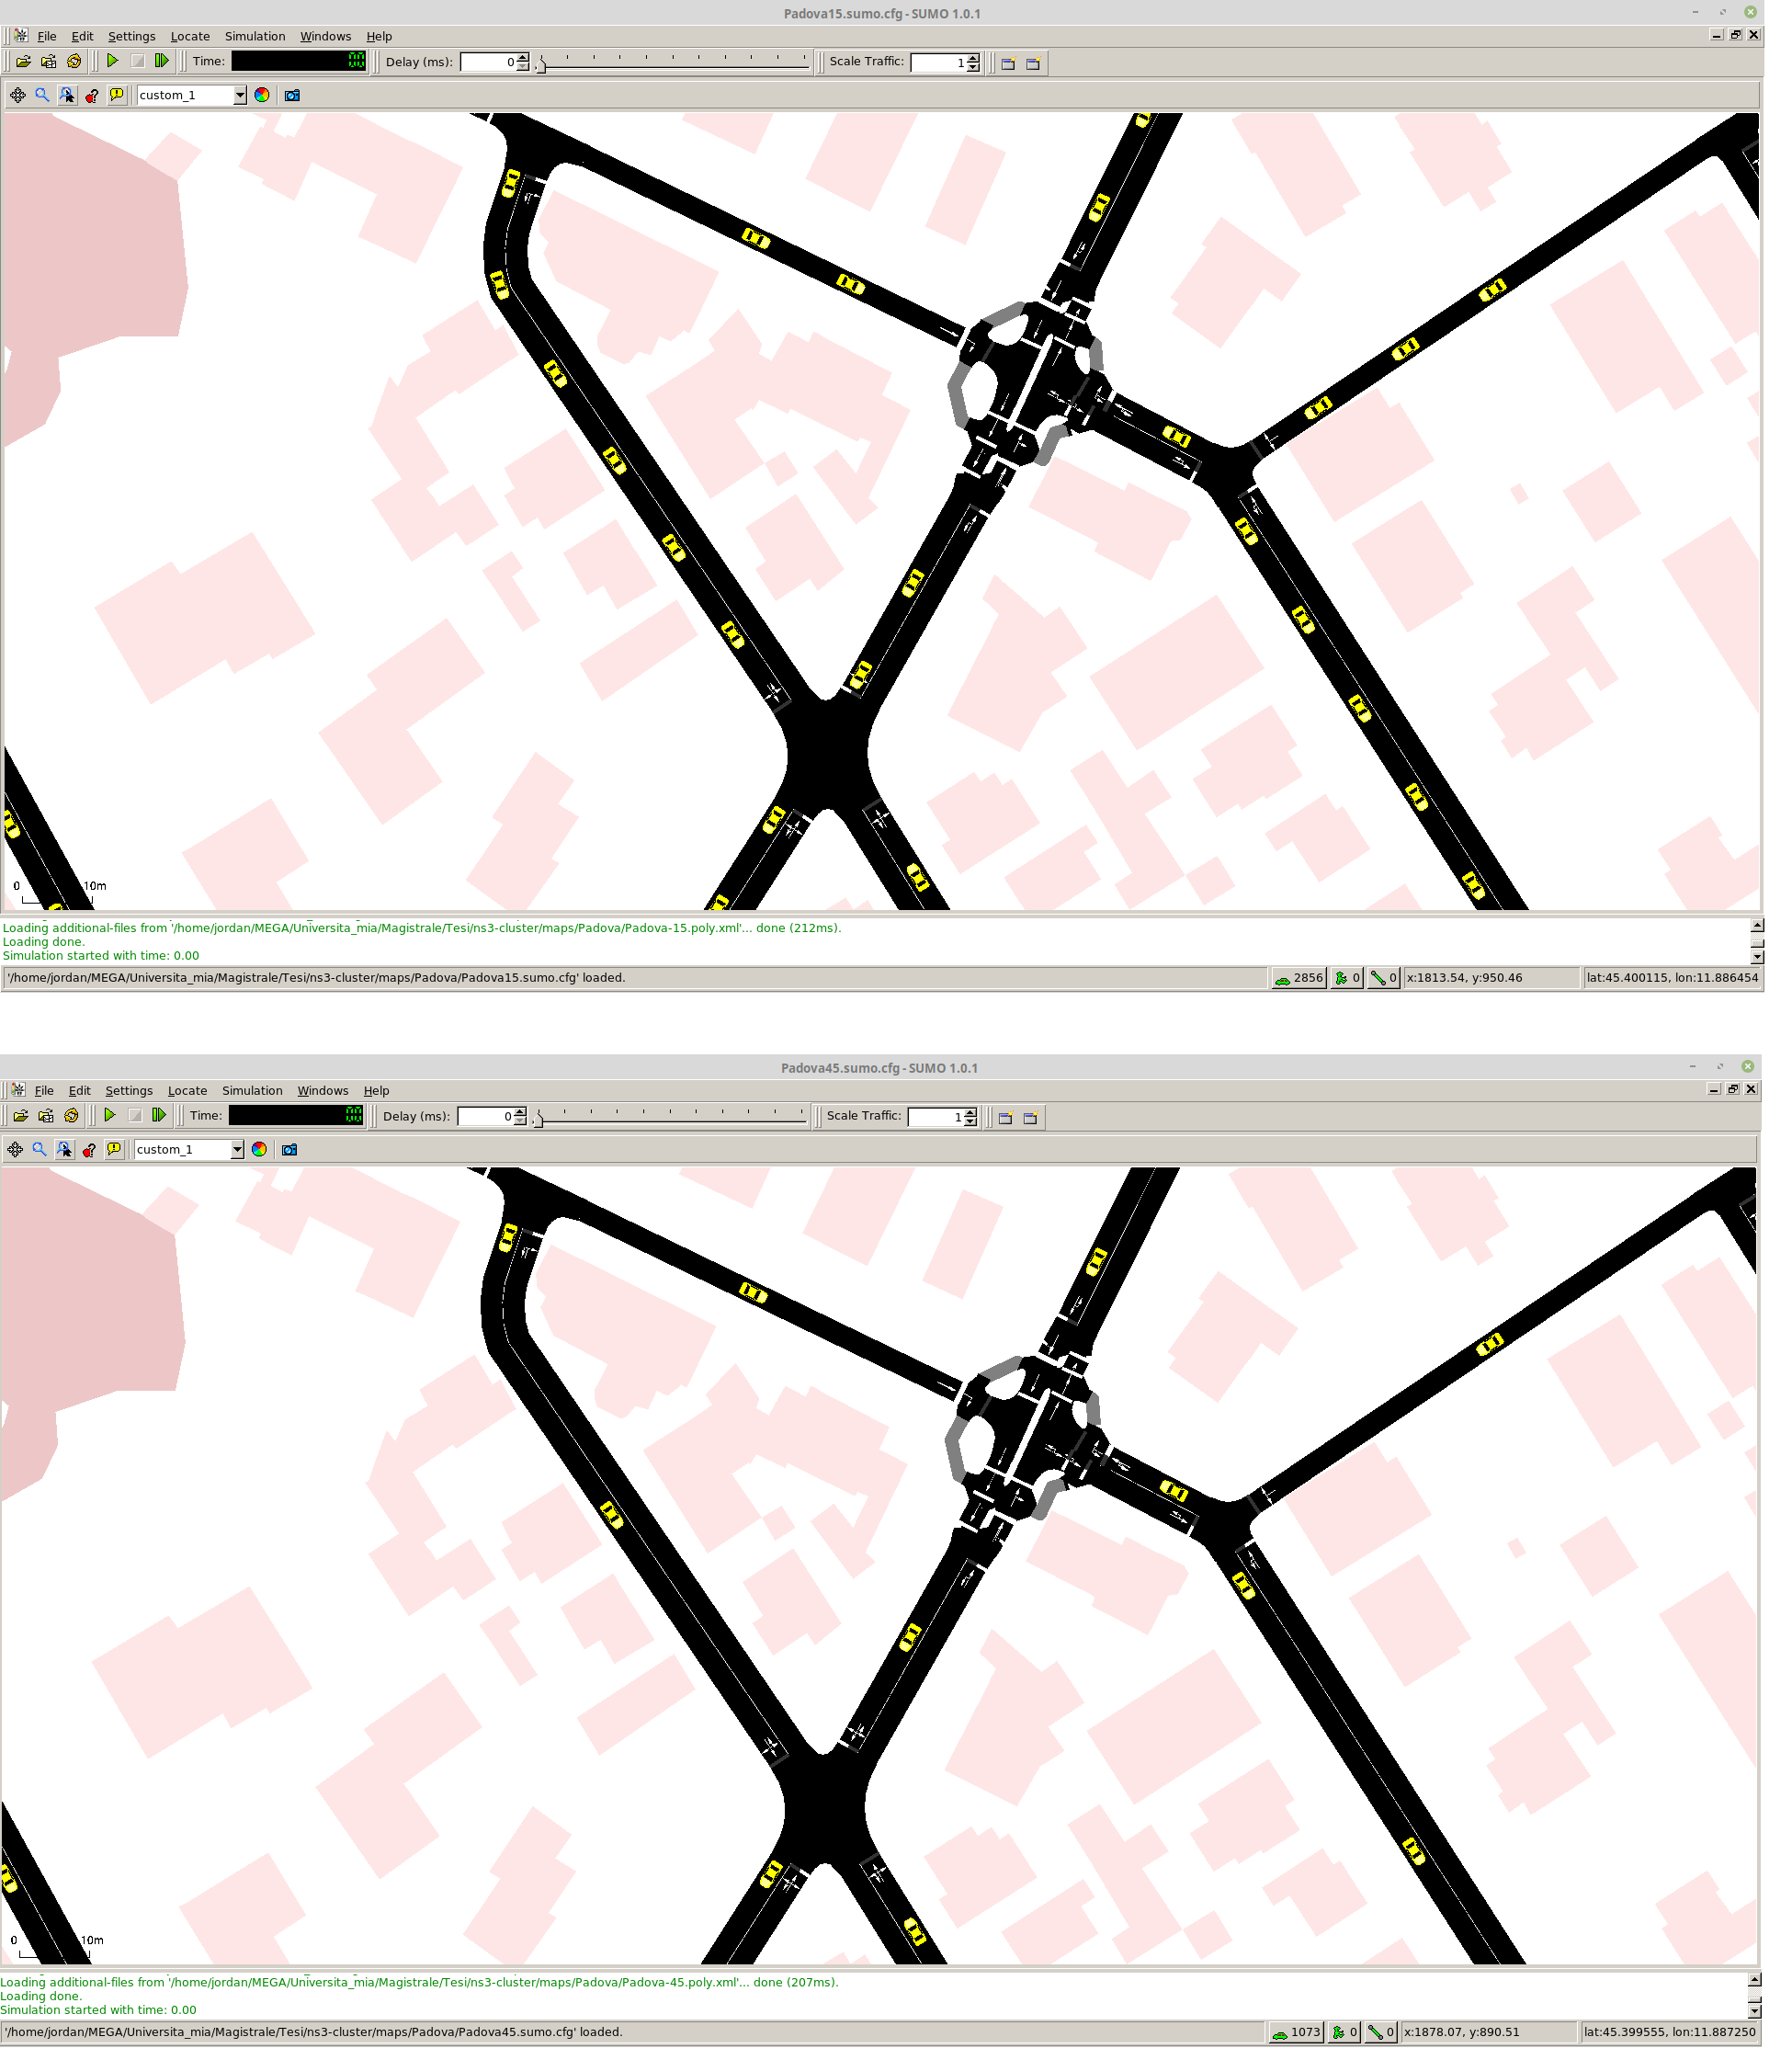
\includegraphics[width=\textwidth]{immagini/sumo-distances}
		\caption{Padua scenario with vehicle distance equals to 15 meters (top) and 45 meters (bottom). Vehicles painted yellow}
		\label{fig:sumo-distances}
	\end{figure}
%\chapter{Svolgimento del progetto}
%\section{Modello di sviluppo}
%	
%	Il modello di sviluppo che ho utilizzanto durante lo svolgimento del progetto è il modello iterativo. Questo modello prevede un'esecuzione ciclica di:
%	\begin{itemize}
%		\item Analisi.
%		\item Progettazione.
%		\item Produzione di prototipi.
%		\item Test.
%		\item Raffinamento dei prototipi.
%	\end{itemize}
%	
%	\begin{figure}[H]
%		\centering
%		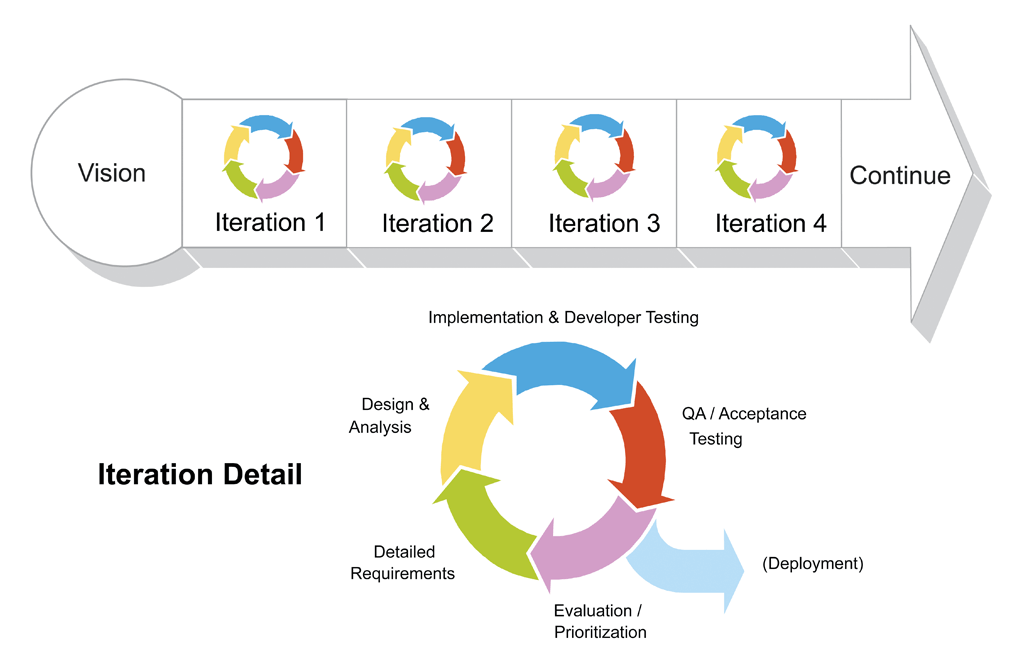
\includegraphics[scale=0.35]{immagini/modello-iterativo}
%		\caption{Modello iterativo (\url{https://goo.gl/YcTb7w}).}
%	\end{figure}
%
%%	Non posso dire di avere utilizzato il modello incrementale in quanto non ho fissato completamente i requisiti e le funzionalità da implementare all'inizio, ma li ho via via ampliati per meglio accomodare le richieste del \textit{tutor}.
%%	Inoltre, ho proceduto con l'implementazione dei \textit{test} automatici solamente nell'ultimo periodo del progetto. Un incremento prevede, oltre all'esecuzione di \textit{test} di unità e integrazione, anche la validazione dell'intero sistema prima di passare allo sviluppo dell'incremento successivo. 
%	
%	Il principale rischio del procedere per iterazioni piuttosto che per \gls{incrementi} è quello di non convergere mai ad una soluzione. Ho quindi adottato delle soluzioni per ridurre questo rischio: 
%	\begin{itemize}
%		\item La prima soluzione è stata fissare con il \textit{tutor} un insieme minimo di requisiti obbligatori da implementare nel prodotto, in modo da avere una soluzione accettabile in un periodo relativamente poco avanzato del progetto.
%		\item La seconda soluzione è stato l'impiego di prototipi da presentare durante gli incontri con il tutor per dare una migliore idea del prodotto in corso di realizzazione.
%	\end{itemize}
%
%	Il procedere per prototipi, oltre ad essere utilizzato ampiamente in IBC, è un metodo che si è rivelato efficace anche nel mio caso. Infatti un prototipo, rispetto alla sola documentazione: 
%	\begin{itemize}
%		\item Fornisce una migliore visione d'insieme del prodotto, garantendo maggiore comprensibilità anche da parte del personale non tecnico.
%		\item Richiede relativamente poco tempo per essere prodotto e modificato, permettendo maggiore flessibilità nel caso di modifiche. Inoltre, diminuisce di molto il tempo che intercorre tra il momento della decisione della modifica e la presentazione del prototipo successivo che la implementa.
%		\item Permette di comprendere meglio anche il \textit{design} grafico e l'esperienza di utilizzo volute dal committente nei periodi iniziali del progetto.
%	\end{itemize}
%	Nei primi periodi i prototipi da me prodotti hanno avuto forma cartacea, per poi evolversi in pagine \textit{web} appena ho preso dimestichezza con Wicket.
%	
%\section{Analisi dei requisiti}
%	Dopo aver completato lo studio di fattibilità e scelto tutte le tecnologie necessarie, ho proceduto a effettuare l'analisi dei requisiti.
%	
%	La metodologia di conduzione dell'analisi che ho utilizzato si è basata principalmente su interviste al \textit{tutor} in modo da identificare innanzitutto i casi d'uso e successivamente i requisiti.
%	
%	Periodicamente ho effettuato incontri con il \textit{tutor} per verificare la corretta comprensione dei requisiti. In questo modo, nonostante io non abbia prodotto documentazione formale sull'analisi, ho ridotto il rischio di incomprensioni difficili da correggere se mantenute durante tutta la durata del processo di sviluppo.
%	
%	Inoltre, per ridurre ulteriormente il rischio di implementare funzionalità non volute o in modo errato, ho prodotto quasi fin da subito dei prototipi da presentare durante gli incontri, come esposto nella sezione precedente.
%	
%	\subsection{Scopo del prodotto}
%		L'applicazione prodotta doveva essere una \textit{web app} che permettesse all'utente di inserire, visualizzare, modificare e rimuovere prodotti commerciali di varie tipologie. L'applicazione doveva considerare categorie e sottocategorie di prodotti. Ad esempio, la pasta è una sottocategorie dei prodotti alimentari.
%		
%		Per ogni prodotto, l'utente doveva essere in grado di inserire le informazioni, obbligatorie od opzionali, imposte dalla categoria di prodotto. Oltre a queste informazioni, l'utente doveva avere la possibilità di inserire un qualsiasi numero di proprietà aggiuntive non previste dalla tipologia.
%		Ogni prodotto poteva avere associata una o più immagini che lo rappresentassero.
%		
%		Opzionalmente, l'applicazione doveva fornire la possibilità di definire da interfaccia anche nuove tipologie e sottotipologie di prodotto.
%	
%	\subsection{Attori}
%		Il primo passo che ho svolto è stato l'identificazione degli attori. Dato che il \textit{tutor} non ha richiesto l'implementazione di gerarchie di utenti o dell'autenticazione, ho identificato solamente un attore, che d'ora in poi chiamerò \jquote{Utente}.
%		
%		\begin{figure}[H]
%			\centering
%			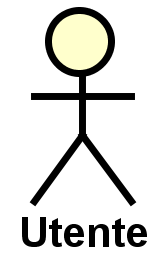
\includegraphics[scale=0.5]{immagini/utente}
%			\caption{Attore utente.}
%		\end{figure}
%		
%	\subsection{Casi d'uso}
%		Una volta identificato l'attore, ho proceduto a identificare le azioni che egli intendeva svolgere utilizzando il prodotto. A scopo esemplificativo, in questa sezione rappresento alcuni casi d'uso che ho identificato..
%		
%%		\begin{figure}[H]
%%			\centering
%%			\includegraphics[width=\textwidth]{{img/uc0.1}.png}
%%			\caption{Panoramica dei casi d'uso - Gestione asset}
%%		\end{figure}
%
%		% !TEX encoding = UTF-8
% !TEX TS-program = pdflatex
% !TEX root = ../tesi.tex
{
%\subsection*{Panoramica generale}  
%\begin{figure}[H] 
%	\centering 
%	\includegraphics[scale=0.4]{"immagini/usecase/Panoramica dei casi d'uso"} 
%	\caption{Esempio di casi d'uso.}
%\end{figure}
%\def\arraystretch{1.5}
%\rowcolors{2}{D}{P}
%\begin{tabularx}{\textwidth}{l|p{0.7\textwidth}}
%	\rowcolor{I} \multicolumn{2}{c}{\color{white}\textbf{UC1 - Aggiunta asset}} \\
%	\toprule
%	\endhead
%	\textbf{Attori} & Utente\\
%	\textbf{Descrizione} & l'utente aggiunge un asset\\
%	\textbf{Pre-condizione} & l'utente ha aperto l'applicazione\\
%	\textbf{Post-condizione} & un nuovo asset è stato aggiunto ed è visualizzabile sulla mappa; l'utente visualizza un messaggio che comunica la corretta esecuzione dell'operazione; l'area informativa rimane impostata sull'asset appena inserito; la posizione e il livello di ingrandimento della mappa rimangono invariati\\
%	\textbf{Scenario principale} & \vspace{-1.2em}
%	\begin{enumerate}[leftmargin=*,noitemsep,nosep]
%		\item \nameref{sssec:UC1.1};
%		\item \nameref{sssec:UC1.2};
%		\item \nameref{sssec:UC1.4}.
%	\end{enumerate}\\
%	\textbf{Estensioni} & \vspace{-1.2em}
%	\begin{itemize}[leftmargin=*,noitemsep,nosep]
%		\item \nameref{sssec:UC30}: l’utente interrompe volontariamente l’aggiunta dell’asset
%	\end{itemize}\\
%	\textbf{Scenari alternativi} & \vspace{-1.2em}
%	\begin{itemize}[leftmargin=*,noitemsep,nosep]
%		\item \nameref{sssec:UC1.3};
%		\item \nameref{sssec:UC1.5}.
%	\end{itemize}\\
%	\textbf{Generalizzazioni} &  \\
%	\bottomrule
%\end{tabularx}

\subsection*{UC1 - Visualizzazione lista prodotti}
	\label{sec:UC1}  
	\begin{figure}[H] 
		\centering 
		\includegraphics[scale=0.35]{"immagini/usecase/UC1 - Visualizzazione lista prodotti"} 
		\caption{UC1 - Visualizzazione lista prodotti.}
	\end{figure}
	\def\arraystretch{1.3}
	\rowcolors{2}{D}{P}
	\begin{tabularx}{\textwidth}{l|p{0.7\textwidth}}
%		\caption{UC1 - Visualizzazione lista prodotti}
		\rowcolor{I} \multicolumn{2}{c}{\color{white}\textbf{UC1 - Visualizzazione lista prodotti}} \\
		\toprule
		\endhead
		\textbf{Attori} & Utente.\\
		\textbf{Descrizione} & L'utente visualizza la lista dei prodotti presenti all'interno dell'applicazione.\\
		\textbf{Pre-condizione} & L'utente ha aperto l'applicazione.\\
		\textbf{Post-condizione} & L'utente ha visualizzato la lista dei prodotti presenti all'interno dell'applicazione.\\
		\textbf{Scenario principale} & \vspace{-1.2em}
		\begin{enumerate}[leftmargin=*,noitemsep,nosep]
			\item \nameref{sec:UC1}.
		\end{enumerate}\\
%		\textbf{Estensioni} & \vspace{-1.2em}
%		\begin{itemize}[leftmargin=*,noitemsep,nosep]
%			\item \nameref{sssec:UC30}: l’utente interrompe volontariamente l’aggiunta dell’asset
%		\end{itemize}\\
%		\textbf{Scenari alternativi} & \vspace{-1.2em}
%		\begin{itemize}[leftmargin=*,noitemsep,nosep]
%			\item \nameref{sssec:UC1.3};
%			\item \nameref{sssec:UC1.5}.
%		\end{itemize}\\
%		\textbf{Generalizzazioni} &  \\
%		\bottomrule
	\end{tabularx}

%\subsection*{UC2 - Visualizzazione dettaglio prodotto}
%	\label{sec:UC2}  
%	\begin{figure}[H] 
%		\centering 
%		\includegraphics[scale=0.6]{"immagini/usecase/UC2 - Visualizzazione dettaglio prodotto"} 
%		\caption{UC2 - Visualizzazione dettaglio prodotto.}
%	\end{figure}
%	\def\arraystretch{1.5}
%	\rowcolors{2}{D}{P}
%	\begin{tabularx}{\textwidth}{l|p{0.7\textwidth}}
%		\rowcolor{I} \multicolumn{2}{c}{\color{white}\textbf{UC2 - Visualizzazione dettaglio prodotto}} \\
%		\toprule
%		\endhead
%		\textbf{Attori} & Utente.\\
%		\textbf{Descrizione} & L'utente visualizza le informazioni di dettaglio di un prodotto.\\
%		\textbf{Pre-condizione} & L'utente ha aperto l'applicazione.\\
%		\textbf{Post-condizione} & L'utente ha visualizzato informazioni di dettaglio di un prodotto.\\
%		\textbf{Scenario principale} & \vspace{-1.2em}
%		\begin{enumerate}[leftmargin=*,noitemsep,nosep]
%			\item \nameref{sec:UC2.1}.
%			\item \nameref{sec:UC2.2}.
%		\end{enumerate}\\
%		%		\textbf{Estensioni} & \vspace{-1.2em}
%		%		\begin{itemize}[leftmargin=*,noitemsep,nosep]
%		%			\item \nameref{sssec:UC30}: l’utente interrompe volontariamente l’aggiunta dell’asset
%		%		\end{itemize}\\
%		%		\textbf{Scenari alternativi} & \vspace{-1.2em}
%		%		\begin{itemize}[leftmargin=*,noitemsep,nosep]
%		%			\item \nameref{sssec:UC1.3};
%		%			\item \nameref{sssec:UC1.5}.
%		%		\end{itemize}\\
%		%		\textbf{Generalizzazioni} &  \\
%		%		\bottomrule
%\end{tabularx}

%\clearpage
%\subsection*{UC2.1 - Visualizzazione nome prodotto}
%\label{sec:UC2.1}  
%%\begin{figure}[H] 
%%	\centering 
%%	\includegraphics[scale=0.6]{"immagini/usecase/UC2 - Visualizzazione dettaglio prodotto"} 
%%	\caption{UC2 - Visualizzazione dettaglio prodotto.}
%%\end{figure}
%\def\arraystretch{1.5}
%\rowcolors{2}{D}{P}
%\begin{tabularx}{\textwidth}{l|p{0.7\textwidth}}
%	\rowcolor{I} \multicolumn{2}{c}{\color{white}\textbf{UC2.1 - Visualizzazione nome prodotto}} \\
%	\toprule
%	\endhead
%	\textbf{Attori} & Utente.\\
%	\textbf{Descrizione} & L'utente visualizza il nome di un prodotto.\\
%	\textbf{Pre-condizione} & L'utente ha aperto l'applicazione.\\
%	\textbf{Post-condizione} & L'utente ha visualizzato il nome di un prodotto.\\
%	\textbf{Scenario principale} & \vspace{-1.2em}
%	\begin{enumerate}[leftmargin=*,noitemsep,nosep]
%		\item \nameref{sec:UC2.1}.
%	\end{enumerate}\\
%	%		\textbf{Estensioni} & \vspace{-1.2em}
%	%		\begin{itemize}[leftmargin=*,noitemsep,nosep]
%	%			\item \nameref{sssec:UC30}: l’utente interrompe volontariamente l’aggiunta dell’asset
%	%		\end{itemize}\\
%	%		\textbf{Scenari alternativi} & \vspace{-1.2em}
%	%		\begin{itemize}[leftmargin=*,noitemsep,nosep]
%	%			\item \nameref{sssec:UC1.3};
%	%			\item \nameref{sssec:UC1.5}.
%	%		\end{itemize}\\
%	%		\textbf{Generalizzazioni} &  \\
%	%		\bottomrule
%\end{tabularx}
%
%\subsection*{UC2.2 - Visualizzazione proprietà prodotto}
%\label{sec:UC2.2}  
%%\begin{figure}[H] 
%%	\centering 
%%	\includegraphics[scale=0.6]{"immagini/usecase/UC2 - Visualizzazione dettaglio prodotto"} 
%%	\caption{UC2 - Visualizzazione dettaglio prodotto.}
%%\end{figure}
%\def\arraystretch{1.5}
%\rowcolors{2}{D}{P}
%\begin{tabularx}{\textwidth}{l|p{0.7\textwidth}}
%	\rowcolor{I} \multicolumn{2}{c}{\color{white}\textbf{UC2.2 - Visualizzazione proprietà prodotto}} \\
%	\toprule
%	\endhead
%	\textbf{Attori} & Utente.\\
%	\textbf{Descrizione} & L'utente visualizza le proprietà di un prodotto.\\
%	\textbf{Pre-condizione} & L'utente ha aperto l'applicazione.\\
%	\textbf{Post-condizione} & L'utente ha visualizzato le proprietà di un prodotto.\\
%	\textbf{Scenario principale} & \vspace{-1.2em}
%	\begin{enumerate}[leftmargin=*,noitemsep,nosep]
%		\item \nameref{sec:UC2.2}.
%	\end{enumerate}\\
%	%		\textbf{Estensioni} & \vspace{-1.2em}
%	%		\begin{itemize}[leftmargin=*,noitemsep,nosep]
%	%			\item \nameref{sssec:UC30}: l’utente interrompe volontariamente l’aggiunta dell’asset
%	%		\end{itemize}\\
%	%		\textbf{Scenari alternativi} & \vspace{-1.2em}
%	%		\begin{itemize}[leftmargin=*,noitemsep,nosep]
%	%			\item \nameref{sssec:UC1.3};
%	%			\item \nameref{sssec:UC1.5}.
%	%		\end{itemize}\\
%	%		\textbf{Generalizzazioni} &  \\
%	%		\bottomrule
%\end{tabularx}
%
%\subsection*{UC3 - Inserimento prodotto}
%\label{sec:UC3}  
%%\begin{figure}[H] 
%%	\centering 
%%	\includegraphics[scale=0.6]{"immagini/usecase/UC3 - Inserimento prodotto"} 
%%	\caption{UC2 - Visualizzazione dettaglio prodotto.}
%%\end{figure}
%\def\arraystretch{1.5}
%\rowcolors{2}{D}{P}
%\begin{tabularx}{\textwidth}{l|p{0.7\textwidth}}
%	\rowcolor{I} \multicolumn{2}{c}{\color{white}\textbf{UC3 - Inserimento prodotto}} \\
%	\toprule
%	\endhead
%	\textbf{Attori} & Utente.\\
%	\textbf{Descrizione} & L'utente inserisce un nuovo prodotto.\\
%	\textbf{Pre-condizione} & L'utente ha aperto l'applicazione.\\
%	\textbf{Post-condizione} & L'utente ha inserito un nuovo prodotto.\\
%	\textbf{Scenario principale} & \vspace{-1.2em}
%	\begin{enumerate}[leftmargin=*,noitemsep,nosep]
%				\item \nameref{sec:UC3}.
%			\end{enumerate}\\
%%	\begin{enumerate}[leftmargin=*,noitemsep,nosep]
%%		\item \nameref{sec:UC3.1}.
%%		\item \nameref{sec:UC3.2}.
%%		\item \nameref{sec:UC3.3}.
%%		\item \nameref{sec:UC3.4}.
%%		\item \nameref{sec:UC3.5}.
%%	\end{enumerate}\\
%
%	%		\textbf{Estensioni} & \vspace{-1.2em}
%	%		\begin{itemize}[leftmargin=*,noitemsep,nosep]
%	%			\item \nameref{sssec:UC30}: l’utente interrompe volontariamente l’aggiunta dell’asset
%	%		\end{itemize}\\
%	%		\textbf{Scenari alternativi} & \vspace{-1.2em}
%	%		\begin{itemize}[leftmargin=*,noitemsep,nosep]
%	%			\item \nameref{sssec:UC1.3};
%	%			\item \nameref{sssec:UC1.5}.
%	%		\end{itemize}\\
%	%		\textbf{Generalizzazioni} &  \\
%	%		\bottomrule
%\end{tabularx}
%
%\subsection*{UC4 - Modifica prodotto}
%\label{sec:UC4}  
%%\begin{figure}[H] 
%%	\centering 
%%	\includegraphics[scale=0.6]{"immagini/usecase/UC2 - Visualizzazione dettaglio prodotto"} 
%%	\caption{UC2 - Visualizzazione dettaglio prodotto.}
%%\end{figure}
%\def\arraystretch{1.5}
%\rowcolors{2}{D}{P}
%\begin{tabularx}{\textwidth}{l|p{0.7\textwidth}}
%	\rowcolor{I} \multicolumn{2}{c}{\color{white}\textbf{UC4 - Modifica prodotto}} \\
%	\toprule
%	\endhead
%	\textbf{Attori} & Utente.\\
%	\textbf{Descrizione} & L'utente modifica le informazioni di un prodotto.\\
%	\textbf{Pre-condizione} & L'utente ha aperto l'applicazione e sta visualizzando le informazioni di un prodotto.\\
%	\textbf{Post-condizione} & L'utente ha modificato le informazioni di un prodotto.\\
%	\textbf{Scenario principale} & \vspace{-1.2em}
%	\begin{enumerate}[leftmargin=*,noitemsep,nosep]
%		\item \nameref{sec:UC4}.
%	\end{enumerate}\\
%	%		\textbf{Estensioni} & \vspace{-1.2em}
%	%		\begin{itemize}[leftmargin=*,noitemsep,nosep]
%	%			\item \nameref{sssec:UC30}: l’utente interrompe volontariamente l’aggiunta dell’asset
%	%		\end{itemize}\\
%	%		\textbf{Scenari alternativi} & \vspace{-1.2em}
%	%		\begin{itemize}[leftmargin=*,noitemsep,nosep]
%	%			\item \nameref{sssec:UC1.3};
%	%			\item \nameref{sssec:UC1.5}.
%	%		\end{itemize}\\
%	%		\textbf{Generalizzazioni} &  \\
%	%		\bottomrule
%\end{tabularx}
%
%\subsection*{UC5 - Eliminazione prodotto}
%\label{sec:UC5}  
%%\begin{figure}[H] 
%%	\centering 
%%	\includegraphics[scale=0.6]{"immagini/usecase/UC2 - Visualizzazione dettaglio prodotto"} 
%%	\caption{UC2 - Visualizzazione dettaglio prodotto.}
%%\end{figure}
%\def\arraystretch{1.5}
%\rowcolors{2}{D}{P}
%\begin{tabularx}{\textwidth}{l|p{0.7\textwidth}}
%	\rowcolor{I} \multicolumn{2}{c}{\color{white}\textbf{UC5 - Eliminazione prodotto}} \\
%	\toprule
%	\endhead
%	\textbf{Attori} & Utente.\\
%	\textbf{Descrizione} & L'utente elimina un prodotto.\\
%	\textbf{Pre-condizione} & L'utente ha aperto l'applicazione e sta visualizzando le informazioni di dettaglio del prodotto.\\
%	\textbf{Post-condizione} & L'utente ha eliminato un prodotto.\\
%	\textbf{Scenario principale} & \vspace{-1.2em}
%	\begin{enumerate}[leftmargin=*,noitemsep,nosep]
%		\item \nameref{sec:UC5}.
%	\end{enumerate}\\
%	%		\textbf{Estensioni} & \vspace{-1.2em}
%	%		\begin{itemize}[leftmargin=*,noitemsep,nosep]
%	%			\item \nameref{sssec:UC30}: l’utente interrompe volontariamente l’aggiunta dell’asset
%	%		\end{itemize}\\
%	%		\textbf{Scenari alternativi} & \vspace{-1.2em}
%	%		\begin{itemize}[leftmargin=*,noitemsep,nosep]
%	%			\item \nameref{sssec:UC1.3};
%	%			\item \nameref{sssec:UC1.5}.
%	%		\end{itemize}\\
%	%		\textbf{Generalizzazioni} &  \\
%	%		\bottomrule
%\end{tabularx}
%
%\subsection*{UC6 - Inserimento nuova tipologia di prodotto}
%\label{sec:UC6}  
%%\begin{figure}[H] 
%%	\centering 
%%	\includegraphics[scale=0.6]{"immagini/usecase/UC2 - Visualizzazione dettaglio prodotto"} 
%%	\caption{UC2 - Visualizzazione dettaglio prodotto.}
%%\end{figure}
%\def\arraystretch{1.5}
%\rowcolors{2}{D}{P}
%\begin{tabularx}{\textwidth}{l|p{0.7\textwidth}}
%	\rowcolor{I} \multicolumn{2}{c}{\color{white}\textbf{UC6 - Inserimento nuova tipologia di prodotto}} \\
%	\toprule
%	\endhead
%	\textbf{Attori} & Utente.\\
%	\textbf{Descrizione} & L'utente inserisce una nuova tipologia di prodotto.\\
%	\textbf{Pre-condizione} & L'utente ha aperto l'applicazione.\\
%	\textbf{Post-condizione} & L'utente ha inserito una nuova tipologia di prodotto.\\
%	\textbf{Scenario principale} & \vspace{-1.2em}
%	\begin{enumerate}[leftmargin=*,noitemsep,nosep]
%		\item \nameref{sec:UC6}.
%	\end{enumerate}\\
%	%		\textbf{Estensioni} & \vspace{-1.2em}
%	%		\begin{itemize}[leftmargin=*,noitemsep,nosep]
%	%			\item \nameref{sssec:UC30}: l’utente interrompe volontariamente l’aggiunta dell’asset
%	%		\end{itemize}\\
%	%		\textbf{Scenari alternativi} & \vspace{-1.2em}
%	%		\begin{itemize}[leftmargin=*,noitemsep,nosep]
%	%			\item \nameref{sssec:UC1.3};
%	%			\item \nameref{sssec:UC1.5}.
%	%		\end{itemize}\\
%	%		\textbf{Generalizzazioni} &  \\
%	%		\bottomrule
%\end{tabularx}
%
%\subsection*{UC7 - Modifica tipologia prodotto}
%\label{sec:UC7}  
%%\begin{figure}[H] 
%%	\centering 
%%	\includegraphics[scale=0.6]{"immagini/usecase/UC2 - Visualizzazione dettaglio prodotto"} 
%%	\caption{UC2 - Visualizzazione dettaglio prodotto.}
%%\end{figure}
%\def\arraystretch{1.5}
%\rowcolors{2}{D}{P}
%\begin{tabularx}{\textwidth}{l|p{0.7\textwidth}}
%	\rowcolor{I} \multicolumn{2}{c}{\color{white}\textbf{UC7 - Modifica tipologia prodotto}} \\
%	\toprule
%	\endhead
%	\textbf{Attori} & Utente.\\
%	\textbf{Descrizione} & L'utente modifica una tipologia di prodotto.\\
%	\textbf{Pre-condizione} & L'utente ha aperto l'applicazione. È presente almeno una tipologia di prodotto all'interno dell'applicazione.\\
%	\textbf{Post-condizione} & L'utente ha modificato una tipologia di prodotto.\\
%	\textbf{Scenario principale} & \vspace{-1.2em}
%	\begin{enumerate}[leftmargin=*,noitemsep,nosep]
%		\item \nameref{sec:UC7}.
%	\end{enumerate}\\
%	%		\textbf{Estensioni} & \vspace{-1.2em}
%	%		\begin{itemize}[leftmargin=*,noitemsep,nosep]
%	%			\item \nameref{sssec:UC30}: l’utente interrompe volontariamente l’aggiunta dell’asset
%	%		\end{itemize}\\
%	%		\textbf{Scenari alternativi} & \vspace{-1.2em}
%	%		\begin{itemize}[leftmargin=*,noitemsep,nosep]
%	%			\item \nameref{sssec:UC1.3};
%	%			\item \nameref{sssec:UC1.5}.
%	%		\end{itemize}\\
%	%		\textbf{Generalizzazioni} &  \\
%	%		\bottomrule
%\end{tabularx}
%
%\subsection*{UC8 - Eliminazione tipologia prodotto}
%\label{sec:UC8}  
%%\begin{figure}[H] 
%%	\centering 
%%	\includegraphics[scale=0.6]{"immagini/usecase/UC2 - Visualizzazione dettaglio prodotto"} 
%%	\caption{UC2 - Visualizzazione dettaglio prodotto.}
%%\end{figure}
%\def\arraystretch{1.5}
%\rowcolors{2}{D}{P}
%\begin{tabularx}{\textwidth}{l|p{0.7\textwidth}}
%	\rowcolor{I} \multicolumn{2}{c}{\color{white}\textbf{UC8 - Eliminazione tipologia prodotto}} \\
%	\toprule
%	\endhead
%	\textbf{Attori} & Utente.\\
%	\textbf{Descrizione} & L'utente elimina una tipologia di prodotto.\\
%	\textbf{Pre-condizione} & L'utente ha aperto l'applicazione. È presente almeno una tipologia di prodotto all'interno dell'applicazione.\\
%	\textbf{Post-condizione} & L'utente ha eliminato una tipologia di prodotto.\\
%	\textbf{Scenario principale} & \vspace{-1.2em}
%	\begin{enumerate}[leftmargin=*,noitemsep,nosep]
%		\item \nameref{sec:UC8}.
%	\end{enumerate}\\
%	%		\textbf{Estensioni} & \vspace{-1.2em}
%	%		\begin{itemize}[leftmargin=*,noitemsep,nosep]
%	%			\item \nameref{sssec:UC30}: l’utente interrompe volontariamente l’aggiunta dell’asset
%	%		\end{itemize}\\
%	%		\textbf{Scenari alternativi} & \vspace{-1.2em}
%	%		\begin{itemize}[leftmargin=*,noitemsep,nosep]
%	%			\item \nameref{sssec:UC1.3};
%	%			\item \nameref{sssec:UC1.5}.
%	%		\end{itemize}\\
%	%		\textbf{Generalizzazioni} &  \\
%	%		\bottomrule
%\end{tabularx}
%
\subsection*{UC2 - Esecuzione ricerca}
\label{sec:UC2}  
\begin{figure}[H] 
	\centering 
	\includegraphics[scale=0.35]{"immagini/usecase/UC2 - Esecuzione ricerca"} 
	\caption{UC2 - Esecuzione ricerca.}
\end{figure}
\def\arraystretch{1.3}
\rowcolors{2}{D}{P}
\begin{tabularx}{\textwidth}{l|p{0.7\textwidth}}
	\rowcolor{I} \multicolumn{2}{c}{\color{white}\textbf{UC2 - Esecuzione ricerca}} \\
	\toprule
	\endhead
	\textbf{Attori} & Utente.\\
	\textbf{Descrizione} & L'utente esegue una ricerca.\\
	\textbf{Pre-condizione} & L'utente ha aperto la schermata di ricerca.\\
	\textbf{Post-condizione} & L'utente ha eseguito la ricerca e ne visualizza i risultati.\\
	\textbf{Scenario principale} & \vspace{-1.2em}
	\begin{enumerate}[leftmargin=*,noitemsep,nosep]
		\item \nameref{sec:UC2}.
	\end{enumerate}\\
	%		\textbf{Estensioni} & \vspace{-1.2em}
	%		\begin{itemize}[leftmargin=*,noitemsep,nosep]
	%			\item \nameref{sssec:UC30}: l’utente interrompe volontariamente l’aggiunta dell’asset
	%		\end{itemize}\\
	%		\textbf{Scenari alternativi} & \vspace{-1.2em}
	%		\begin{itemize}[leftmargin=*,noitemsep,nosep]
	%			\item \nameref{sssec:UC1.3};
	%			\item \nameref{sssec:UC1.5}.
	%		\end{itemize}\\
	%		\textbf{Generalizzazioni} &  \\
	%		\bottomrule
\end{tabularx}
}    
%	
%	\subsection{Requisiti}
%		\label{sec:requisiti}
%		Successivamente, dopo aver identificato i casi d'uso, ho provveduto a trasformarli in requisiti elementari che descrivessero le caratteristiche che il prodotto avrebbe dovuto avere.
%		
%		Rendere elementari i requisiti scendendo ad un basso livello di dettaglio è importante per aumentarne la comprensibilità e garantirne l'atomicità, ovvero fare in modo che essi si riferiscano ad una singola e precisa necessità senza alcuna ambiguità.
%		
%		Nella tabella di seguito fornisco un elenco di alto livello delle principali funzionalità, ricavate dall'analisi dei requisiti, che l'applicazione doveva offrire. Ad ogni funzionalità è associata una certa importanza (obbligatoria, desiderabile o facoltativa).
%%		Ogni requisito è identificato con un codice univoco, secondo la seguente notazione:
%%		\begin{center}
%%			R[Importanza][Tipologia][Codice]
%%		\end{center}
%%		L'\textbf{importanza} indica quanto gli \gls{stakeholder} valutano quel requisito. Può assumere i seguenti valori:
%%		\begin{itemize}
%%			\item \textbf{O:} indica un requisito obbligatorio.
%%			\item \textbf{D:} indica un requisito desiderabile.
%%			\item \textbf{F:} indica un requisito facoltativo.
%%		\end{itemize}
%%		La \textbf{tipologia} indica la categoria di appartenenza del requisito. Può assumere uno tra i seguenti valori:
%%		\begin{itemize}
%%			\item \textbf{F:} indica un requisito funzionale;
%%%			\item \textbf{Q:} indica un requisito di qualità;
%%%			\item \textbf{P:} indica un requisito prestazionale;
%%			\item \textbf{V:} indica un requisito di vincolo.
%%		\end{itemize}
%%		Il \textbf{codice} è un valore numerico progressivo.
%%		
%		% !TEX encoding = UTF-8
% !TEX TS-program = pdflatex
% !TEX root = ../tesi.tex

\begin{tabularx}{\textwidth}{|l|l|}
	\hline
	 \textbf{Funzionalità} & \textbf{Importanza} \\
	\hline
	Gestione prodotti & Obbligatoria\\
	\hline
	Gestione immagine prodotto & Desiderabile\\
	\hline
	Gestione categorie prodotti & Facoltativa\\
	\hline
	Gestione catalogo immagini prodotti & Facoltativa\\
	\hline
	\caption{Principali funzionalità ricavate dai requisiti.}
\end{tabularx}  
%		
%
%\section{Progettazione}
%
%	Per quanto riguarda la progettazione, ho seguito un approccio \jquote{\textit{meet-in-the-middle}}, ovvero ho utilizzato sia l'approccio \textit{top-down} che \textit{bottom-up}.
%	
%	Il motivo di questa scelta è dovuto a esperienze passate vissute durante lo svolgimento del progetto di \gls{swe}. Infatti, io e il mio \textit{team} avevamo progettato in modo puramente \textit{top-down} senza avere una conoscenza profonda delle tecnologie utilizzate. La conseguenza è stata una progettazione che impiegava \textit{design pattern} non adatti alle tecnologie, la quale ha causato ritardi dovuti alla riprogettazione necessaria a risolvere gli errori.
%	
%	Per non ripetere lo stesso errore, sono arrivato anche a progettare e codificare alcune componenti di basso livello prima di fissare completamente l'intera architettura. Questa scelta ha avuto un duplice vantaggio:
%	\begin{itemize}
%		\item In primo luogo, mi ha permesso di convergere ad una soluzione architetturale funzionante e che si adattava bene alle tecnologie utilizzate.
%		\item In secondo luogo, la codifica delle componenti grafiche mi ha permesso di avere dei prototipi in periodi relativamente poco avanzati del progetto, con i vantaggi descritti nelle sezioni precedenti.
%	\end{itemize}
%	
%	L'architettura del prodotto si basa sul \textit{design pattern} \textit{Model-View-Controller}, alla cui base c'è il principio di separazione delle responsabilità. Questa scelta si adatta anche al \textit{framework} Wicket, che effettua già una prima separazione della \textit{View} fornendo pagine HTML statiche da popolare tramite codice Java.
%	
%	\begin{figure}[H]
%		\centering
%		\includegraphics[width=\textwidth]{immagini/mvc}
%		\caption{Rappresentazione dell'architettura MVC con \textit{pattern} Observer. (\url{https://goo.gl/NYKkpQ}).}
%	\end{figure}
%
%	\subsection{DAO}
%		L'accesso ai dati contenuti nel JCR richiede l'utilizzo di API di relativamente basso livello per la lettura e la scrittura. Per separare ulteriormente la logica dell'applicazione da queste API, ho utilizzato il \textit{design pattern} Data Access Object (DAO).
%		
%		Questo \textit{pattern} consiste nel racchiudere tutte le operazioni che effettuano l'accesso ad un \textit{database} (in questo caso, il JCR) in apposite classi. Gli oggetti di queste classi nascondono l'esistenza di \textit{query} fornendo dei metodi che restituiscono oggetti di \textit{business} utilizzabili direttamente dall'applicazione.
%		
%		\begin{figure}[H]
%			\centering
%			\includegraphics[scale=0.4]{immagini/dao}
%			\caption{Ruolo del DAO nell'architettura.}
%		\end{figure}
%	
%	\subsection{Struttura JCR}
%		Ho progettato la struttura del contenuto del JCR sotto forma di albero, così come previsto dal modello JCR.
%		
%		Ogni elemento memorizzato è definito come nodo dell'albero. Ogni nodo può avere delle proprietà e ogni proprietà a sua volta ha un valore. I dati concreti sono memorizzati solamente come valore di una proprietà, le quali diventano quindi le foglie dell'albero.
%		
%		Includo un esempio minimale di struttura di JCR. Nella rappresentazione, i nodi hanno una forma circolare mentre le proprietà assumono una forma rettangolare.
%		
%		\begin{figure}[H]
%			\centering
%			\includegraphics[scale=0.9]{immagini/esempiostrutturajcr}
%			\caption{Esempio struttura JCR.}
%		\end{figure}
%	
%	\subsection{\textit{View}}
%		Durante la progettazione della \textit{View} ho sfruttato i componenti \texttt{Panel} di Wicket per massimizzare il riuso di codice.
%		
%		Un \texttt{Panel} infatti può essere utilizzato in diversi punti dell'applicazione senza la necessità di dover ricopiare il \textit{markup} ogni volta. Fornisco un piccolo esempio di progettazione di due pagine diverse che utilizzano lo stesso \texttt{Panel}.
%		
%		\begin{figure}[H]
%			\centering
%			\includegraphics[width=\textwidth]{immagini/pnl}
%			\caption{Esempio di utilizzo di \texttt{Panel} di Wicket.}
%		\end{figure}
%	
%		Un altro esempio di utilizzo dei \texttt{Panel} è in combinazione con i componenti \texttt{Repeater}, i quali permettono di creare un componente grafico per ogni elemento presente all'interno di una collezione.
%			
%\section{Codifica}
%	Ho realizzato il prodotto utilizzando i seguenti linguaggi:
%	\begin{itemize}
%		\item \textbf{Java 8:} per l'utilizzo delle API JCR e la realizzazione della \textit{View} con Wicket.
%		\item \textbf{HTML5:} per la creazione del \textit{markup} delle componenti Wicket.
%		\item \textbf{CSS:} per assegnare lo stile alle pagine \textit{web}.
%		\item \textbf{XML:} per la configurazione di Maven.
%		\item \textbf{Compact Namespace and Node Type Definition (CND):} per la definizione dei tipi di nodo e della struttura di JCR. 
%	\end{itemize}	
%	Nonostante Jackrabbit offrisse API aggiuntive rispetto al JCR, ho utilizzato principalmente quelle specificate dallo \textit{standard} \gls{jsr283}, contenute all'interno di \texttt{javax.jcr.*}. Questa scelta assicura:
%	\begin{itemize}
%		\item Maggiore compatibilità con altre implementazioni di JCR nel caso di sostituzione della libreria Jackrabbit con un'altra libreria.
%		\item Minori problemi in caso di aggiornamento della libreria Jackrabbit, in quanto le API definite dallo \textit{standard} possono cambiare solamente a causa di un aggiornamento dello \textit{standard} stesso. Le API di Jackrabbit invece possono cambiare molto più facilmente e senza preavviso.
%	\end{itemize}
%	Durante la codifica in Java ho utilizzato alcune caratteristiche del linguaggio che non avevo appreso durante gli studi universitari, tra cui:
%	\begin{itemize}
%		\item \textbf{Java Annotations:} una forma di metadato da associare ad un qualche elemento del codice in modo da fornire maggiore leggibilità da parte di altri sviluppatori e sopratuttto da parte del compilatore. Alcune delle \textit{annotation} che ho utilizzato maggiormente sono state \texttt{@Override} per la ridefinizione dei metodi e \texttt{@Test} per la specifica dei \textit{test case}.
%		\item \textbf{\textit{Reflection}:} meccanismo tramite il quale è possibile ottenere informazioni sul codice e modificare metodi, classi e attributi a \textit{runtime}. La \textit{reflection} viene utilizzata sopratutto da Wicket.
%	\end{itemize}
%	Per quanto riguarda la rappresentazione degli oggetti di \textit{business}, ho utilizzato dei JavaBean. Questi ultimi sono degli oggetti di classi sottoposte a vari vincoli, tra cui avere solo il costruttore di \textit{default} e permettere l'accesso ai propri campi dati attraverso metodi \texttt{get} e \texttt{set}. Quest'ultimo vincolo, unito alla \textit{reflection}, permette a Wicket di legare i campi dati dei \textit{bean} ai valori dei componenti grafici, in modo da permettere inserimenti e visualizzazioni dei dati.
%
%	Per meglio documentare il codice ho prodotto, attraverso l'utilizzo di Javadoc, una pagina \textit{web} che fornisce descrizioni di classi e metodi.
%
%		
%\section{Verifica e validazione}
%	Durante tutto lo svolgimento del progetto ho eseguito attività di verifica. Le revisioni periodiche con il \textit{tutor} e i colleghi durante le quali ho dimostrato prototipi, documentazione ed esempi di codice sorgente sono state utili a verificare che il progetto procedesse secondo quanto pianificato. Inoltre, le verifiche sono state utili per la risoluzione dei problemi che ho incontrato durante la codifica.
%	
%	\subsection{\textit{Test}}
%	Un altro tipo di verifica che ho impiegato è quella automatica tramite \textit{test} utilizzando JUnit4. Nonostante io abbia eseguito i \textit{test} di sistema solamente nel periodo finale del progetto, ho effettuato verifiche più mirate tramite \textit{test} di unità nel corso del progetto, sopratutto per quanto riguarda le componenti della \textit{View}. L'utilizzo di \texttt{WicketTester} ha permesso \textit{test} di unità di componenti Wicket senza troppo dispendio di tempo.
%	
%	Per evitare di dover ridefinire i meccanismi di funzionamento del JCR durante l'esecuzione dei \textit{test} di integrazione, ho utilizzato la classe \texttt{JackrabbitRepositoryStub} fornita da Jackrabbit. Questa classe fornisce uno \gls{stub} di un JCR; l'ho utilizzata per testare l'interazione delle altre componenti con il \textit{repository}.
%	
%	I \textit{test} di integrazione e di sistema che interagiscono con la \textit{View} sono guidati da un oggetto della classe \texttt{WicketTester}, che permette la simulazione di eventi come l'inserimento di caratteri da tastiera o la pressione di un bottone.
%	
%	Una delle difficoltà principali che ho incontrato durante l'esecuzione dei \textit{test} di sistema è stata l'interazione tra eventi Ajax e l'invio di \textit{form}. \texttt{WicketTester} infatti fornisce un oggetto di tipo \texttt{FormTester}, che permette l'impostazione di valori degli oggetti contenuti in una data \textit{form} e il successivo invio della stessa. Data la mia inesperienza con gli eventi Ajax, ho impiegato un po' di tempo durante il periodo finale del progetto per capirne il funzionamento e completare i \textit{test} in maniera corretta. Anche grazie all'aiuto della \textit{mailing list} di Wicket, sono riuscito a risolvere i problemi incontrati e ad implementare la maggior parte dei \textit{test} previsti. 
%%	Fornisco un elenco dei \textit{test} di sistema pianificati ed eseguiti, utilizzando le seguenti abbreviazioni:
%%	\begin{itemize}
%%		\item \textbf{NI:} non implementato.
%%		\item \textbf{I:} implementato.
%%		\item \textbf{NS:} non superato.
%%		\item \textbf{S:} superato.
%%	\end{itemize}
%%	
%%	% !TEX encoding = UTF-8
% !TEX TS-program = pdflatex
% !TEX root = ../tesi.tex
{
	\def\arraystretch{1.5}
	\rowcolors{2}{D}{P}
	\begin{longtable}{p{1.5cm}!{\VRule[1pt]}p{5cm}!{\VRule[1pt]}p{1cm}!{\VRule[1pt]}p{1cm}}
		\rowcolor{I}
		\color{white} \textbf{Test} & \color{white} \textbf{Descrizione} & \color{white} \textbf{Stato} & \color{white} \textbf{Esito} \\ 
		\endfirsthead 
		\rowcolor{I} 
		\color{white} \textbf{Test} & \color{white} \textbf{Descrizione} & \color{white} \textbf{Stato} & \color{white} \textbf{Esito} \\ 
		\endhead 
		TS1 & Viene verificato che il sistema permetta la visualizzazione dei prodotti. & \impl & \super \\ 
		TS2 & Viene verificato che il sistema permetta l'inserimento di un prodotto. & \impl & \super \\
		TS3 & Viene verificato che il sistema permetta la modifica di un prodotto. & \impl & \super \\
		TS4 & Viene verificato che il sistema permetta l'eliminazione di un prodotto. & \impl & \super \\
		TS5 & Viene verificato che il sistema permetta l'esecuzione di una ricerca. & \impl & \super \\
		TS6 & Viene verificato che il sistema permetta la visualizzazione dei risultati di una ricerca & \impl & \super \\ 
		TS7 & Viene verificato che il sistema permetta l'associazione di un'immagine ad un prodotto. & \impl & \super \\ 
		TS8 & Viene verificato che il sistema permetta l'associazione di un catalogo di immagini ad un prodotto. & \nonimpl & \nonsuper \\
		TS9 & Viene verificato che il sistema permetta l'inserimento di una nuova tipologia di prodotto. & \nonimpl & \nonsuper \\
		\caption{Test di sistema.}
	\end{longtable}
}  
%%	
%
%	Grazie al \textit{plug-in} EclEmma per Eclipse ho potuto calcolare i gradi di copertura del codice da parte dei \textit{test}. Complessivamente, \textit{test} di unità, integrazione e sistema hanno dato i seguenti risultati:
%	\begin{table}[H]
%		\centering
%		\begin{tabular}{|c|c|}
%			\hline
%			\textbf{Tipo di \textit{coverage}} & \textbf{Percentuale} \\
%			\hline
%			\gls{statementcoverage} & 85\% \\
%			\hline
%			\gls{branchcoverage} & 80\%\\
%			\hline
%		\end{tabular}
%		\caption{Resoconto copertura del codice.}
%	\end{table}
%	Durante la pianificazione e l'implementazione dei \textit{test} ho preferito testare più profondamente le funzionalità di maggior importanza e a maggior rischio di errore, dati anche i vincoli temporali dello \textit{stage}. Per questo motivo le percentuali di copertura non raggiungono il 100\%, ma si attestano in ogni caso su risultati accettabili.
%	
%	\subsubsection{\textit{Test} prestazionali}
%	Uno degli obiettivi del prototipo era l'implementazione di ricerche \textit{full-text} tra gli elementi inseriti. Il \textit{tutor} si è dimostrato interessato alla valutazione prestazionale delle due tipologie di ricerca offerte da JCR:
%	\begin{itemize}
%		\item La ricerca \jquote{classica}, ovvero eseguita tramite operatore \texttt{LIKE}.
%		\item La ricerca \textit{full-text} eseguita tramite operatore \texttt{CONTAINS}.
%	\end{itemize}
%	
%	Ho eseguito \textit{test} prestazionali su un insieme di 20.000 prodotti di tipo pasta strutturati nel seguente modo:
%	\begin{table}[H]
%		\centering
%		\begin{tabular}{|c|c|}
%			\hline
%			\textbf{Nome attributo} & \textbf{Tipo attributo JCR} \\
%			\hline
%			id & \texttt{String} \\
%			\hline
%			prezzo & \texttt{Decimal} \\
%			\hline
%			minutiCottura & \texttt{Long} \\
%			\hline
%			volume & \texttt{Decimal} \\
%			\hline
%			marca & \texttt{String} \\
%			\hline
%		\end{tabular}
%		\caption{Descrizione struttura prodotto utilizzato nei \textit{test} prestazionali.}
%	\end{table}
%	
%	Eseguendo per dieci volte \textit{query} equivalenti, ovvero che ritornavano lo stesso insieme di risultati, ho ottenuto i seguenti risultati:
%	
%	\begin{table}[H]
%		\centering
%		\begin{tabular}{|c|c|c|c|c|c|c|c|c|c|c|c|}
%			\hline
%			\textbf{Operatore} & \multicolumn{10}{c|}{\textbf{Tempo di esecuzione (ms)}} & \textbf{Media} \\
%			\hline 
%			& \multicolumn{10}{c|}{\textbf{Numero \textit{test}}} & \\
%			\hline 
%			& \textbf{1} & \textbf{2} & \textbf{3} & \textbf{4} & \textbf{5} & \textbf{6} & \textbf{7} & \textbf{8} & \textbf{9} & \textbf{10} & \\
%			\hline 
%			CONTAINS & 396 & 476 & 528 & 292 & 805 & 687 & 436 & 557 & 418 & 510 & \green{510,50} \\
%			\hline 
%			LIKE & 503 & 636 & 697 & 432 & 531 & 747 & 807 & 873 & 772 & 651& \red{665,90} \\
%			\hline 
%		\end{tabular}
%		\caption{Resoconto \textit{test} prestazionali.}
%	\end{table}
%	
%	Come dimostrato dai \textit{test}, l'operatore \texttt{CONTAINS} restituisce i risultati impiegando mediamente un tempo minore del 23\% rispetto all'operatore \texttt{LIKE}. Il motivo di questa differenza è dovuta al fatto che Jackrabbit sfrutta il motore di ricerca testuale fornito da Apache Lucene per l'esecuzione delle ricerche \textit{full-text} con l'operatore \texttt{CONTAINS}. Questo motore è conosciuto per la sua velocità in questo tipo di ricerche.
%	
%	Ho prodotto un documento destinato a IBC che illustra il procedimento utilizzato per effettuare i \textit{test} prestazionali e i risultati ottenuti.
%	
%	\subsubsection{Validazione}
%	
%	Ho eseguito attività di validazione durante gli ultimi giorni dello \textit{stage} mostrando il prodotto al \textit{tutor} e dimostrandogli le funzionalità implementate. Grazie ai \textit{test} di sistema che avevo precedentemente eseguito ho potuto portare a termine la validazione in sicurezza, avendo la garanzia che il sistema rispondesse correttamente ai casi d'uso previsti. Complessivamente, la validazione ha avuto esito positivo.
%
%\section{Prodotto finale}
%	Il prodotto finale assume la forma di una \textit{web app} \textit{single-page}. Per istruire l'utilizzatore finale all'utilizzo del prodotto ho redatto un manuale utente comprensivo di immagini. 
%	
%	Procedo a illustrare alcune funzionalità offerte dal prodotto.
%	
%	\subsection{\textit{Homepage}}
%		L'\textit{homepage} presenta una tabella con struttura ad albero tramite la quale è possibile visualizzare le informazioni dei prodotti. Cliccando sul pulsante \jquote{+} è possibile espandere la visualizzazione delle categorie, fino ad arrivare alla visualizzazione dei prodotti desiderati.
%		
%		\begin{figure}[H]
%			\centering
%			\includegraphics[width=\textwidth]{immagini/home-page-blank}
%			\caption{\textit{Homepage} con nessun prodotto visualizzato.}
%		\end{figure}
%	
%		\begin{figure}[H]
%			\centering
%			\includegraphics[width=11cm]{immagini/homepage-view-product}
%			\caption{\textit{Homepage} con alcuni prodotti visualizzati.}
%		\end{figure}
%	
%	\subsection{Finestra di inserimento}
%		La finestra di inserimento permette di aggiungere nuovi prodotti a partire dalle categorie già esistenti. Selezionando la tipologia di prodotto, l'applicazione come prima cosa richiede la compilazione dei campi dati predefiniti. Quelli obbligatori sono segnalati da un asterisco di colore rosso.
%		
%		Una volta compilati i dati obbligatori, l'utente ha la possibilità di aggiungere proprietà aggiuntive tramite l'utilizzo del pulsante \jquote{Aggiungi riga proprietà}. Una proprietà consiste di tre elementi:
%		\begin{itemize}
%			\item Un nome.
%			\item Un tipo, a scelta fra \texttt{String}, \texttt{Long}, \texttt{Decimal}, \texttt{Double}.
%			\item Un valore, in accordo con il tipo scelto.
%		\end{itemize}
%		Infine, l'utente ha la possibilità di aggiungere una sola immagine da abbinare al prodotto.
%		
%		\begin{figure}[H]
%			\centering
%			\includegraphics[width=\textwidth]{immagini/add-page}
%			\caption{Finestra di inserimento prodotto.}
%		\end{figure}
%	
%	\subsection{Finestra di visualizzazione dettaglio e modifica}
%		Cliccando sul pulsante \jquote{Modifica} affianco al nome di un prodotto verrà aperta la finestra di visualizzazione dettaglio e modifica.
%		
%		All'interno di questa finestra l'utente ha la possibilità di:
%		\begin{itemize}
%			\item Visualizzare e modificare le informazioni di dettaglio del prodotto.
%			\item Rimuovere eventuali proprietà aggiuntive precedentemente inserite. Le proprietà predefinite non possono essere rimosse per non invalidare la struttura imposta dalla categoria del prodotto.
%			\item Aggiungere ulteriori proprietà.
%			\item Visualizzare e modificare l'immagine che rappresenta il prodotto.
%		\end{itemize}
%		
%		\begin{figure}[H]
%			\centering
%			\includegraphics[width=\textwidth]{immagini/edit-page}
%			\caption{Finestra di visualizzazione dettaglio e modifica prodotto.}
%		\end{figure}
%	
%	\subsection{Finestra di ricerca}
%		Dalla finestra di ricerca l'utente può effettuare ricerche tra i prodotti, raffinando i criteri di selezione fino ad arrivare all'articolo (o all'insieme di articoli) di interesse.
%		
%		Per effettuare una ricerca è necessario seguire i seguenti passi:
%		\begin{itemize}
%			\item Come prima cosa, l'applicazione richiede che venga selezionata una tipologia di prodotto su cui fare la ricerca. Le tipologie suggerite sono tutte quelle presenti all'interno del JCR in quel dato momento. Se la tipologia non viene specificata, la ricerca comprenderà i prodotti di tutte le categorie.  
%			\item Successivamente, l'utente potrà aggiungere uno o più filtri di ricerca, specificando per ognuno:
%				\begin{itemize}
%					\item \textbf{Nome della proprietà da ricercare}. L'applicazione suggerisce tutte le proprietà definite dalla struttura della tipologia di prodotto selezionato, più eventuali proprietà aggiuntive.
%					\item \textbf{Operatore da applicare}, come ad esempio >, >=, <, <=, =.
%					\item \textbf{Valore da ricercare}.
%				\end{itemize}	
%			\item Una volta eseguita la ricerca, i risultati verranno visualizzati nella stessa finestra. L'utente è libero di modificare e rimuovere i filtri precedentemente utilizzati, oppure di inserirne di nuovi per raffinare la ricerca. 	
%		\end{itemize}
%		
%		\begin{figure}[H]
%			\centering
%			\includegraphics[height=7.1cm, width=\textwidth]{immagini/query-page-doppio}
%			\caption{Finestra di ricerca, filtro di selezione multiplo.}
%		\end{figure}
%	
%		Per accedere alla funzionalità di ricerca \textit{full-text}, è sufficiente selezionare la voce \jquote{Tutte} nel \textit{box} che indica la proprietà da ricercare. Così facendo, l'unico operatore disponibile sarà \texttt{CONTAINS}, il quale cercherà il testo immesso dall'utente all'interno di tutte le proprietà di tipo \texttt{String} di tutti i nodi della tipologia specificata.
%		
%		\begin{figure}[H]
%			\centering
%			\includegraphics[height=7.1cm, width=\textwidth]{immagini/query-page-contains}
%			\caption{Finestra di ricerca, filtro di selezione \textit{full-text}.}
%		\end{figure}            
%% !TEX encoding = UTF-8
% !TEX TS-program = pdflatex
% !TEX root = ../tesi.tex

%**************************************************************
\chapter{Analisi dei requisiti}
\label{cap:analisi-requisiti}
%**************************************************************

\intro{Breve introduzione al capitolo}\\

\section{Casi d'uso}

Per lo studio dei casi di utilizzo del prodotto sono stati creati dei diagrammi.
I diagrammi dei casi d'uso (in inglese \emph{Use Case Diagram}) sono diagrammi di tipo \gls{uml} dedicati alla descrizione delle funzioni o servizi offerti da un sistema, così come sono percepiti e utilizzati dagli attori che interagiscono col sistema stesso.
Essendo il progetto finalizzato alla creazione di un tool per l'automazione di un processo, le interazioni da parte dell'utilizzatore devono essere ovviamente ridotte allo stretto necessario. Per questo motivo i diagrammi d'uso risultano semplici e in numero ridotto.

\begin{figure}[!h] 
    \centering 
    \includegraphics[width=0.9\columnwidth]{usecase/scenario-principale} 
    \caption{Use Case - UC0: Scenario principale}
\end{figure}

\begin{usecase}{0}{Scenario principale}
\usecaseactors{Sviluppatore applicativi}
\usecasepre{Lo sviluppatore è entrato nel plug-in di simulazione all'interno dell'IDE}
\usecasedesc{La finestra di simulazione mette a disposizione i comandi per configurare, registrare o eseguire un test}
\usecasepost{Il sistema è pronto per permettere una nuova interazione}
\label{uc:scenario-principale}
\end{usecase}

\section{Tracciamento dei requisiti}

Da un'attenta analisi dei requisiti e degli use case effettuata sul progetto è stata stilata la tabella che traccia i requisiti in rapporto agli use case.\\
Sono stati individuati diversi tipi di requisiti e si è quindi fatto utilizzo di un codice identificativo per distinguerli.\\
Il codice dei requisiti è così strutturato R(F/Q/V)(N/D/O) dove:
\begin{enumerate}
	\item[R =] requisito
    \item[F =] funzionale
    \item[Q =] qualitativo
    \item[V =] di vincolo
    \item[N =] obbligatorio (necessario)
    \item[D =] desiderabile
    \item[Z =] opzionale
\end{enumerate}
Nelle tabelle \ref{tab:requisiti-funzionali}, \ref{tab:requisiti-qualitativi} e \ref{tab:requisiti-vincolo} sono riassunti i requisiti e il loro tracciamento con gli use case delineati in fase di analisi.

\newpage

\begin{table}%
\caption{Tabella del tracciamento dei requisti funzionali}
\label{tab:requisiti-funzionali}
\begin{tabularx}{\textwidth}{lXl}
\hline\hline
\textbf{Requisito} & \textbf{Descrizione} & \textbf{Use Case}\\
\hline
RFN-1     & L'interfaccia permette di configurare il tipo di sonde del test & UC1 \\
\hline
\end{tabularx}
\end{table}%

\begin{table}%
\caption{Tabella del tracciamento dei requisiti qualitativi}
\label{tab:requisiti-qualitativi}
\begin{tabularx}{\textwidth}{lXl}
\hline\hline
\textbf{Requisito} & \textbf{Descrizione} & \textbf{Use Case}\\
\hline
RQD-1    & Le prestazioni del simulatore hardware deve garantire la giusta esecuzione dei test e non la generazione di falsi negativi & - \\
\hline
\end{tabularx}
\end{table}%

\begin{table}%
\caption{Tabella del tracciamento dei requisiti di vincolo}
\label{tab:requisiti-vincolo}
\begin{tabularx}{\textwidth}{lXl}
\hline\hline
\textbf{Requisito} & \textbf{Descrizione} & \textbf{Use Case}\\
\hline
RVO-1    & La libreria per l'esecuzione dei test automatici deve essere riutilizzabile & - \\
\hline
\end{tabularx}
\end{table}%           
%% !TEX encoding = UTF-8
% !TEX TS-program = pdflatex
% !TEX root = ../tesi.tex

%**************************************************************
\chapter{Analisi dei requisiti}
\label{cap:analisi-requisiti}
%**************************************************************

\intro{Breve introduzione al capitolo}\\

\section{Casi d'uso}

Per lo studio dei casi di utilizzo del prodotto sono stati creati dei diagrammi.
I diagrammi dei casi d'uso (in inglese \emph{Use Case Diagram}) sono diagrammi di tipo \gls{uml} dedicati alla descrizione delle funzioni o servizi offerti da un sistema, così come sono percepiti e utilizzati dagli attori che interagiscono col sistema stesso.
Essendo il progetto finalizzato alla creazione di un tool per l'automazione di un processo, le interazioni da parte dell'utilizzatore devono essere ovviamente ridotte allo stretto necessario. Per questo motivo i diagrammi d'uso risultano semplici e in numero ridotto.

\begin{figure}[!h] 
    \centering 
    \includegraphics[width=0.9\columnwidth]{usecase/scenario-principale} 
    \caption{Use Case - UC0: Scenario principale}
\end{figure}

\begin{usecase}{0}{Scenario principale}
\usecaseactors{Sviluppatore applicativi}
\usecasepre{Lo sviluppatore è entrato nel plug-in di simulazione all'interno dell'IDE}
\usecasedesc{La finestra di simulazione mette a disposizione i comandi per configurare, registrare o eseguire un test}
\usecasepost{Il sistema è pronto per permettere una nuova interazione}
\label{uc:scenario-principale}
\end{usecase}

\section{Tracciamento dei requisiti}

Da un'attenta analisi dei requisiti e degli use case effettuata sul progetto è stata stilata la tabella che traccia i requisiti in rapporto agli use case.\\
Sono stati individuati diversi tipi di requisiti e si è quindi fatto utilizzo di un codice identificativo per distinguerli.\\
Il codice dei requisiti è così strutturato R(F/Q/V)(N/D/O) dove:
\begin{enumerate}
	\item[R =] requisito
    \item[F =] funzionale
    \item[Q =] qualitativo
    \item[V =] di vincolo
    \item[N =] obbligatorio (necessario)
    \item[D =] desiderabile
    \item[Z =] opzionale
\end{enumerate}
Nelle tabelle \ref{tab:requisiti-funzionali}, \ref{tab:requisiti-qualitativi} e \ref{tab:requisiti-vincolo} sono riassunti i requisiti e il loro tracciamento con gli use case delineati in fase di analisi.

\newpage

\begin{table}%
\caption{Tabella del tracciamento dei requisti funzionali}
\label{tab:requisiti-funzionali}
\begin{tabularx}{\textwidth}{lXl}
\hline\hline
\textbf{Requisito} & \textbf{Descrizione} & \textbf{Use Case}\\
\hline
RFN-1     & L'interfaccia permette di configurare il tipo di sonde del test & UC1 \\
\hline
\end{tabularx}
\end{table}%

\begin{table}%
\caption{Tabella del tracciamento dei requisiti qualitativi}
\label{tab:requisiti-qualitativi}
\begin{tabularx}{\textwidth}{lXl}
\hline\hline
\textbf{Requisito} & \textbf{Descrizione} & \textbf{Use Case}\\
\hline
RQD-1    & Le prestazioni del simulatore hardware deve garantire la giusta esecuzione dei test e non la generazione di falsi negativi & - \\
\hline
\end{tabularx}
\end{table}%

\begin{table}%
\caption{Tabella del tracciamento dei requisiti di vincolo}
\label{tab:requisiti-vincolo}
\begin{tabularx}{\textwidth}{lXl}
\hline\hline
\textbf{Requisito} & \textbf{Descrizione} & \textbf{Use Case}\\
\hline
RVO-1    & La libreria per l'esecuzione dei test automatici deve essere riutilizzabile & - \\
\hline
\end{tabularx}
\end{table}%             % Concept Preview
%% !TEX encoding = UTF-8
% !TEX TS-program = pdflatex
% !TEX root = ../tesi.tex

%**************************************************************
\chapter{Progettazione e codifica}
\label{cap:progettazione-codifica}
%**************************************************************

\intro{Breve introduzione al capitolo}\\

%**************************************************************
\section{Tecnologie e strumenti}
\label{sec:tecnologie-strumenti}

Di seguito viene data una panoramica delle tecnologie e strumenti utilizzati.

\subsection*{Tecnologia 1}
Descrizione Tecnologia 1.

\subsection*{Tecnologia 2}
Descrizione Tecnologia 2

%**************************************************************
\section{Ciclo di vita del software}
\label{sec:ciclo-vita-software}

%**************************************************************
\section{Progettazione}
\label{sec:progettazione}

\subsubsection{Namespace 1} %**************************
Descrizione namespace 1.

\begin{namespacedesc}
    \classdesc{Classe 1}{Descrizione classe 1}
    \classdesc{Classe 2}{Descrizione classe 2}
\end{namespacedesc}


%**************************************************************
\section{Design Pattern utilizzati}

%**************************************************************
\section{Codifica}
             % Product Prototype
%% !TEX encoding = UTF-8
% !TEX TS-program = pdflatex
% !TEX root = ../tesi.tex

%**************************************************************
\chapter{Verifica e validazione}
\label{cap:verifica-validazione}
%**************************************************************             % Product Design Freeze e SOP
%% !TEX encoding = UTF-8
% !TEX TS-program = pdflatex
% !TEX root = ../tesi.tex

%**************************************************************
\chapter{Conclusioni}
\label{cap:conclusioni}
%**************************************************************

%**************************************************************
\section{Consuntivo finale}

%**************************************************************
\section{Raggiungimento degli obiettivi}

%**************************************************************
\section{Conoscenze acquisite}

%**************************************************************
\section{Valutazione personale}
             % Conclusioni
%\appendix                               
%% !TEX encoding = UTF-8
% !TEX TS-program = pdflatex
% !TEX root = ../tesi.tex

%**************************************************************
\chapter{Appendice A}
%**************************************************************

\epigraph{Citazione}{Autore della citazione}



             % Appendice A

%**************************************************************
% Materiale finale
%**************************************************************
\backmatter
\printglossaries
% !TEX encoding = UTF-8
% !TEX TS-program = pdflatex
% !TEX root = ../tesi.tex

%**************************************************************
% Bibliografia
%**************************************************************

\cleardoublepage
\chapter{Bibliografia}

\nocite{*}
% Stampa i riferimenti bibliografici
\printbibliography[heading=subbibliography,title={Riferimenti bibliografici},type=book]

% Stampa i siti web consultati
\printbibliography[heading=subbibliography,title={Siti web consultati},type=online]


\end{document}